\chapter{Schéma collaboratif pour résoudre SMEPC}
\minitoc
\newpage
\label{Heuristique}
%	\section{Introduction}
\section{Motivations}

%	\section{Motivations}
La synchronisation efficace de processus hétérogènes reste une question difficile lorsqu'il s'agit de programmation et d'acheminement (voir \cite{article_synchro2}).
%, 18
Elle se pose par exemple dans la gestion des systèmes de partage de véhicules, des drones et des camions dans le contexte de la logistique urbaine, et des processus d'assemblage industriel. Les modèles de programmation linéaire en nombres entiers sont faussés par de grands écarts induits par l'assouplissement de la contrainte d'intégrité (Méthode du Big M). De même, il est difficile de concevoir des systèmes du type \textit{ Branch and Bound} en raison de l'absence d'un système  efficace de génération de bornes. En outre, les exigences de synchronisation augmentent l'impact de l'incertitude et mettent en jeu la robustesse, ce qui rend l'efficacité des heuristiques globales difficile à vérifier. Une façon de résoudre ces problèmes est d'introduire de la flexibilité et de la modularité dans la conception des algorithmes et de s'appuyer sur des schémas de décomposition \textit{adaptés} afin d'émuler les mécanismes d'interaction qui permettent à des acteurs distincts de faire fonctionner un processus complexe de manière décentralisée.  

L'algorithme de programmation dynamique décrit au chapitre précédent implique un trop grand nombre d'états car il devient vite exponentiel en fonction de la taille de l'instance, ce qui nécessite une très grande mémoire. De plus, on a du mal à apporter une modification à ce programme dynamique car il est « \textit{lourd} ».

%me
%	\item besoin de modularité
Nous allons expliquer ici la manière dont le modèle \textbf{SMEPC} présenté auparavant peut être décomposé de façon à reproduire comment les décisions vont être prises dans le cas (réaliste) où la décision est prise en collaboration. Ceci signifie que le directeur de production et le conducteur du véhicule sont des acteurs indépendants qui doivent interagir. L'idée principale à l'œuvre est qu'un conducteur de véhicule décentralisé a pour comportement naturel de se déplacer comme s'il était sûr d'avoir assez de carburant chaque fois qu'il se rend à la micro-usine, il s'adapte alors au contexte réel en attendant d'être rechargé retardant ainsi certains déplacements. Le comportement induit du directeur de production consistera à assurer le plus possible la demande, en faisant un compromis entre la qualité de service et le coût de production. 

Dans ce chapitre, on décrit une décomposition du problème \textbf{SMEPC} à l'aide de deux modèles qui interagiront : le modèle nommé \textbf{Vehicle-Driver (VD)}  présenté à la \textbf{section} \ref{modele_VD} et le modèle nommé \textbf{Production Manager (PM)} présenté à la \textbf{section} \ref{modele_PM}. On étudie \textbf{VD} et \textbf{PM}, du point de vue algorithmique respectivement à la \textbf{section} \ref{algo_VD} et à la \textbf{section} \ref{algo_PM}. Nous y allons aussi décrire les schémas de programmation dynamique \textbf{DPS\_VD} et \textbf{DPS\_PM} que nous proposons pour résoudre respectivement le problème \textbf{VD} et le problème \textbf{PM}. Pour diminuer le nombre d'états généré par l'algorithme \textbf{DPS\_PM}, on va comme au chapitre précédent définir des règles de filtrages exactes et heuristiques. On conçoit un schéma algorithmique collaboratif qu'on nomme \textbf{Pipe-line VD\_PM} qui met en œuvre la décomposition Demandeur/Producteur à la \textbf{section} \ref{algo_VD_PM}. On fait des expérimentations numériques à la \textbf{section} \ref{Expe_VD_PM}, qui visent à évaluer la qualité des solutions obtenus par le schéma collaboratif. 
\section{Le problème du véhicule : \textit{Vehicle-Driver} (VD)}
\label{modele_VD}
Dans cette section, on va commencera par présenter le modèle \textbf{VD} puis on donnera les résultats de complexité du modèle \textbf{VD}. 
\subsection{Le modèle VD}

Partant du problème global désigné par \textbf{SMEPC}, on décide de faire abstraction de l'aspect planification de la production en supposant qu'il y a suffisamment d'hydrogène à la micro-usine pour alimenter le véhicule, peu importe le nombre de fois qu'il ira se recharger. Il se pose le problème de savoir à quelle date (entre quelles stations $j$ et $j+1$) le véhicule se rechargera et en quelle quantité d'hydrogène ? Afin d'apporter des éléments de réponse à ces questions, on décide de concevoir un algorithme DPS qui fonctionne en \textit{Backward}. Dans cette section, pour présenter le modèle \textbf{VD}, on va d'abord lister les entrées du modèle \textbf{VD}, ensuite, on va présenter ce qu'est une solution du modèle \textbf{VD} et enfin, on va présenter la fonction objectif du modèle \textbf{VD}.

Dans le chapitre précédent, on a présenté toutes les entrées du modèle \textbf{SMEPC} (voir le tableau (\ref{inputs_SMEPC})). Le tableau (\ref{inputs_pb_recharge}) résume les entrées du problème \textbf{Vehicle-Driver (VD)} qui est un sous-problème du problème \textbf{SMEPC}. 

\begin{table}[H]
	\centering
	\begin{tabular}{|*{2}{m{8cm}|}}
		\hline
	\rowcolor{cyan}	Noms & Significations\\
		\hline
		$M$  & Nombre de stations (Dépôt exclut)   \\
		\hline
		$\Gamma=(Depot=0, 1, \dots, M, Depot=M+1)$  & Tournée fixe du véhicule (sans les recharges)  \\
		\hline
		$TMax$  & Le délai maximal pour que le véhicule puisse effectuer sa tournée \\
		\hline
		$C^{Veh}$  & Capacité du réservoir d'hydrogène du véhicule   \\
		\hline
		$E_0$  & Charge initiale d'hydrogène du véhicule \\
		\hline
		$p$  & Durée de la recharge du véhicule \\
		\hline
		Pour $j=0, \dots, M$, $ t_j$ & Temps nécessaire pour aller de la station $j$ à la station $j + 1$ \\
		\hline
		Pour $j=0, \dots, M$, $ d_j$ & Temps nécessaire pour aller de la station $j$ à la micro-usine  \\
		\hline
		Pour $j=0, \dots, M $, $d_j^*$  & Temps nécessaire pour aller de la micro-usine à la station $j$    \\
		\hline
		Pour $j=0, \dots, M $, $e_j$ & Energie nécessaire pour aller de la station $j$ à la station $j + 1$ \\
		\hline
		Pour $j=0, \dots, M $, $\varepsilon_j$ & Energie nécessaire pour aller de la station $j$ à la micro-usine \\
		\hline
		Pour $j=0, \dots, M $, $\varepsilon_j^*$ & Energie nécessaire pour aller de la micro-usine à la station $j $  \\
		\hline
	\end{tabular}
	\caption[Entrées du problème VD]{Entrées correspondantes au problème \textbf{VD}. \label{inputs_pb_recharge}}
\end{table}

On oublie ici les restrictions liées à la production d'hydrogène : nous faisons comme si la micro-usine était capable de fournir, à tout moment, au véhicule autant d'énergie qu'il en a besoin. Notre objectif est alors de fixer la stratégie de recharge du véhicule, c'est-à-dire le vecteur de valeurs booléennes $x = (x_j, j = 0, \dots, M)$ et le vecteur de charge $L = (L_j, j = 0, \dots, M)$ du modèle \textbf{SMEPC}, qui nous indiquent respectivement entre quelles stations $j$ et $j+1$ le véhicule se rechargera, et de quelle quantité d'hydrogène. Les variables $T = (T_j, j = 0, \dots, M + 1)$, $T^*= (T^*_j, j = 0, \dots, M + 1)$ et $V^{Veh} = (V^{Veh}_j, j = 0, \dots, M + 1)$ peuvent être considérées comme des variables auxiliaires, dont les valeurs dérivent de $x$ et $L$. Nous faisons les hypothèses suivantes dans le modèle VD : 
\begin{itemize}[label=$\square$]
	\item Le véhicule n'attend jamais : il se recharge en carburant lorsqu'il arrive à la micro-usine, et il garde entre-temps sa vitesse maximale ;
	\item A chaque fois que le véhicule se recharge, (sauf à la dernière recharge) il fait le plein de son réservoir. A la dernière recharge, il se recharge de telle manière qu'il retourne à la micro-usine avec une charge finale au moins égale à $E_0$.
\end{itemize}

De ces constats, on peut dire que les variables $T$, $T^*$ et $V^{Veh}$ signifient : 
\begin{itemize}[label=$\square$]
\item $T= (T_j, j=0, \dots, M+1)$, la valeur entière non négative  $T_j$ représente la date d'arrivée du véhicule à la station $j$ ;
\item $T^*= (T^*_j, j=0, \dots, M+1)$, la valeur entière non négative $T^*_j$ est la date à laquelle le véhicule commence à se recharger en hydrogène entre la station $j$ et la station $j + 1$ si $x_j=1$ ; 
\item $V^{Veh} = (V^{Veh}_j, j=0, \dots, M+1)$, la valeur entière non négative $V^{Veh}_j$ représente la quantité d'hydrogène dans le réservoir du véhicule lorsqu'il arrive à la station $j$.
\end{itemize}
Les contraintes du véhicule sont les contraintes (\ref{1}), (\ref{2}), (\ref{3}), (\ref{4}), (\ref{5}), (\ref{6}) du modèle \textbf{SMEPC}. Il reste à préciser le critère de performance. Bien entendu, il doit inclure le terme $\alpha \times T_{M+1}$. Mais il doit également comporter un élément qui reflète le coût économique de la \textbf{stratégie de recharge optimale} $(x, L)$. Comme nous ne savons pas à l'avance quelle sera la \textbf{stratégie de production}, nous introduisons un coefficient de coût auxiliaire $\beta$ et considérons que le coût économique de la \textbf{stratégie de recharge optimale} $(x, L)$ est la quantité $\beta \times (\sum_j L_j\times x_j)$. Ce coefficient va être un élément clé de l'interaction entre le véhicule (demandeur) et la micro-usine (producteur). %Il en résulte \textbf{VD} : le modèle \textit{Vehicle-Driver}.

 Le modèle du conducteur du véhicule (\textbf{VD}) calcule la \textbf{stratégie de recharge optimale} $(x, L)$, et déduit les variables auxiliaires $ T = (T_j, j = 0, \dots, M + 1)$, $T^*= (T^*_j, j = 0, \dots, M + 1)$ et $V^{Veh} = (V^{Veh}_j, j = 0, \dots, M + 1)$, de telle sorte que :
\begin{itemize}[label=$\square$]
	\item Les contraintes imposées au véhicule dans le modèle \textbf{SMEPC} soient satisfaites ;
	\item La quantité $\alpha \times T_{M + 1} + \beta \times (\sum_j L_j\times x_j)$ soit la plus petite possible.
\end{itemize}

\begin{Example}
	\label{ex_rech_1}	
Le tableau (\ref{ex_rech_1_inst}) donne les distances $t_j$, $d_j$, $d^*_j$, et les énergies $e_j$, $\varepsilon_j$, $\varepsilon^*_j$ d'une instance du modèle \textbf{VD}. Les autres données de l'instance sont : $M=4$, $\Gamma = (0,1 ,2 ,3 ,4 , 5=0)$, $TMax=60$, $C^{Veh}=24$, $E_0=21$, $p=4$. La solution de cette instance est donnée par le tableau (\ref{ex_rech_1_soluti}). Le véhicule se recharge  deux fois. Le véhicule se recharge entre la station $3$ et la station $4$ puis entre la station $4$ et la station $5=0$ d'une quantité d'hydrogène respectivement de $12$ et $22$.
	
	\begin{table}[H]%instance0
		\centering
		\begin{tabular}{|*{7}{m{2cm}|}}
			\hline
			$j$  &0 &1 &2 &3 &4 & 5=0\\
			\hline
			$t_j$  &4 &5 & 7& 6& 5& *\\
		
			\hline
			$d_j=d^*_j$  &1 &4 & 6& 3& 5& 1 \\
			
			\hline
			$e_j$  &5 &6 & 	7& 	7& 	7& *\\
		
			\hline
			$\varepsilon_j=\varepsilon^*_j$  &1 &4 & 8& 3& 6& 1 \\
			\hline
		\end{tabular}
		\caption[Une instance du modèle VD]{Une instance du modèle. \textbf{VD}} \label{ex_rech_1_inst}}
	\end{table}


	\begin{table}[H]
	\centering
	\begin{tabular}{|*{6}{m{2cm}|}}
		\hline
		$j$  &0 &1 &2 &3 &4\\
		\hline
		$x_j$  &0 &0 & 0& 1& 1\\
		
		\hline
		$L_j$  &0 &0 & 0& 12& 22 \\
		\hline
	\end{tabular}
	\caption[La stratégie de recharge optimale de l'instance  du modèle VD du tableau (\ref{ex_rech_1_inst})]{La stratégie de recharge optimale de l'instance  du modèle VD du tableau (\ref{ex_rech_1_inst}). \label{ex_rech_1_soluti}}
\end{table}
	
\end{Example}

\begin{Example}
\label{ex_rech_2}	
	Le tableau (\ref{ex_rech_2_inst}) donne les distances $t_j$, $d_j$, $d^*_j$, et les énergies $e_j$, $\varepsilon_j$, $\varepsilon^*_j$ d'une instance du modèle \textbf{VD}. Les autres données de l'instance sont : $M=10$, $\Gamma = (0,1 ,2 ,3 ,4 , 5,6,7,8,9,10,11=0)$, $TMax=150$, $C^{Veh}=35$, $E_0=5$, $p=5$. La solution de cette instance est donnée par le tableau (\ref{ex_rech_2_soluti}). Le véhicule se recharge  quatre fois. Le véhicule se recharge d'abord, entre la station $0$ et la station $1$, ensuite, entre la station $2$ et la station $3$, ensuite, entre la station $3$ et la station $4$ et enfin entre la station $7$ et la station $8$ d'une quantité d'hydrogène respectivement de $26$, $8$, $34$ et $28$.
		
	\begin{table}%instance170
		\centering
		\begin{tabular}{|*{13}{c|}}
			\hline
			$j$  &0 &1 &2 &3 &4&5&6&7&8&9&10 & 11=0\\
			\hline
			$t_j$& 12& 10 &3& 3& 3& 8&10 &9&	5&6&6&*\\
			\hline
			$d_j=d^*_j$  &1 &11 & 1& 3& 3& 3&10&8&6&7&7& 1\\
			\hline
			$e_j$  &16 &14 & 3& 3& 	3& 10&10&12&5&6&6&*\\
		
			\hline
			$\varepsilon_j=\varepsilon^*_j$ &1 &15 &1 & 4& 3& 4& 14 &8&8&9&7&1\\
		
			\hline
		\end{tabular}
		\caption[Une instance du modèle VD]{Une instance du modèle \textbf{VD}}. \label{ex_rech_2_inst}}
\end{table}

\begin{table}[H]
\centering
\begin{tabular}{|*{12}{c|}}
	\hline
		$j$  &0 &1 &2 &3 &4&5&6&7&8&9&10 \\
	\hline
	$x_j$  &1 &0 & 1& 1& 0&0 &0&1&0&0&0\\
	
	\hline
	$L_j$  &26 &0 & 8& 34& 0&0 &0&28&0&0&0 \\
	\hline
\end{tabular}
\caption[La stratégie de recharge optimale de l'instance  du modèle VD du tableau (\ref{ex_rech_2_inst})]{La stratégie de recharge optimale de l'instance  du modèle VD du tableau (\ref{ex_rech_2_inst}). \label{ex_rech_2_soluti}}
\end{table}
\end{Example}
\poubelle{\subsection{Extensions du modèle VD}
En modifiant certaines caractéristiques (la quantité d'hydrogène rechargée, la durée de la recharge, etc) du modèle \textbf{VD}, on obtient ses variantes :
\begin{itemize}[label=$\square$]
	\item  On peut supposer que le véhicule recharge chaque fois une quantité d'hydrogène soit nulle ou soit égale à une constante $R$;
	\item On peut supposer que le véhicule recharge chaque fois une quantité d'hydrogène variable  de telle sorte qu'on fait le plein du réservoir (c'est le modèle VD);
	\item  On peut supposer que le temps de recharge du véhicule est fixe ;
	\item On peut supposer qu'il existe des dates de recharges interdites ;
	\item On peut supposer que la quantité d'hydrogène chargée est variable, le temps de recharge du véhicule est fixe et qu'il existe des dates de recharges interdites.
\end{itemize}
}
%	\subsection{Formulation linéaire de VD}
\subsection{Complexité du modèle VD avec $L_j$ fixe}


\begin{theo}
	\label{vd_ndhard}
	Si nous imposons que tout $L_j$ est soit nul ou égal à une constante $R$, alors \textbf{VD} devient NP-Hard.
\end{theo}
La démonstration de ce théorème se trouve en annexe à la section \ref{vd_ndhard_section}.




%18/01/2022
\poubelle{
Pour conclure cette partie, on va maintenant présenter une autre méthode de modélisation du problème \textbf{VD} en un problème de plus court chemin dans un graphe $G$.
Le problème \textbf{VD}, si le véhicule fait le plein à chaque recharge, peut être modélisé sous forme d'un graphe orienté $G=(V,U)$ qui se construit de la façon suivante :
\begin{enumerate}
	\item Les nœuds de $G$ sont les éléments de $V$. $V=(j, j=\{0,\dots, M\})$ ;
	
	\item  Les arcs de $G$ sont les éléments de $U$. $U$ se construit de la façon suivante : soit $k \in V$ et $j \in V$, on place un arc du nœud $k$ vers le nœud $j$ si :
	\begin{enumerate}
	\item Le véhicule peut partir de la micro-usine avec le réservoir plein ;
\item	Puis arriver sur le successeur de la station $k$ (la station $k+1$) ; 
\item	Puis traverser les stations $k+2, k+3, \dots, j$ ; 
\item	Et enfin revenir à la micro-usine sans s'être recharger au cours de ce trajet ;
	\end{enumerate}
	%on dit que le véhicule traverse les stations $0,k+1,k+2, \dots, j ,0$  sans se recharger.
	
	Autrement dit, $(k,j) \in U $ si $\varepsilon^*_{k+1}+\sum_{l=k+1}^{j-1}e_{l}+\varepsilon_{j}\leq C^{veh}$ 
	
%	si $k\neq0$ alors $(k,j) \in U $ si $\varepsilon^*_{k+1}+\sum_{l=k+1}^{j-1}e_{l}+\varepsilon_{j}\leq C^{veh}$ 
	
%	et,
	
%	si $k=0$ alors $\varepsilon^*_{1}+\sum_{l=1}^{j-1}e_{l}+\varepsilon_{j}\leq E_{0}$.
\end{enumerate}
Lorsque la capacité du véhicule est infinie le graphe $G$ est complet sinon on supprimera certains arcs en fonction de la valeur de $E_0$.
Le \textbf{plus court chemin} dans $G$ est la solution optimale au problème des recharges (en faisant le plein à chaque fois) d'un véhicule. Le coût est calculé sur chaque arc $(k,j)$ par la somme énergie et temps pondéré respectivement par les coefficients $\alpha$ et $\beta$.

\begin{Example}
	Le graphe G de la figure (\ref{G_graph}) a été construit avec les valeurs $M = 4$, $C^{Veh} = 6$, $E_0 = 3$, $\beta= 1$, et les valeurs $e$, $\varepsilon$ données par le tableau (\ref{Table_VD-Subgraph}) (nous ne mentionnons pas ici les valeurs de temps $t$, $d$, $TMax$). Les chiffres en rouge représentent les composantes énergétiques des coûts.
	
		\begin{figure}[H]
		\centerline{
			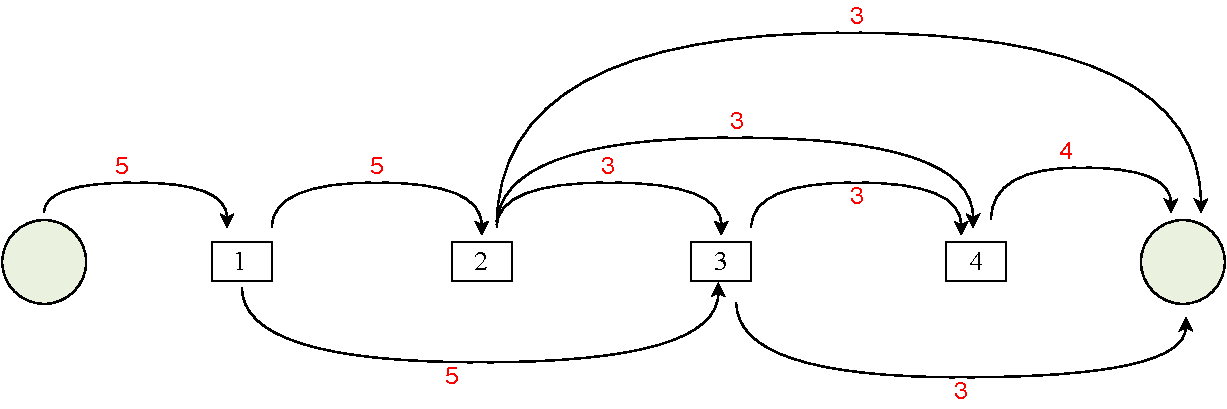
\includegraphics[height=6.3cm]{images_these/G_Graph.pdf}}
		\caption[Le graphe G]{Le graphe G.}
		\label{G_graph}
	\end{figure}
\end{Example}

\begin{Rem}
	En posant $\alpha =1$ et $\beta=0$ on obtient le vecteur $Temps$ et en posant $\alpha=0$ et $\beta=1$ on obtient le vecteur $Energie$ de la section \ref{TempsEnergie} du chapitre précédent.
\end{Rem}
}
\subsection{Complexité du modèle VD avec $L_j$ variable}
\begin{theo}
	\label{VD_polynomial}
	\textbf{VD} peut être résolu en temps polynomial.
\end{theo}
La démonstration de ce théorème se trouve en annexe à la section \ref{VD_polynomial_section}.

\section{Le problème de production : \textit{Production-Manager} (PM)}
\label{modele_PM}
Dans cette section, on commencera par décrire le modèle \textbf{PM}, puis on présentera les résultats de complexité du modèle \textbf{PM}.
\subsection{Le modèle PM}
Dans le chapitre précédent, on a présenté les entrées du modèle \textbf{SMEPC}. Le tableau (\ref{inputs_pb_production}) résume les entrées du problème PM qui est un sous-problème du problème \textbf{SMEPC}.

\begin{table}[H]
	\centering
	\begin{tabular}{|*{2}{m{8cm}|}}
		\hline
	\rowcolor{cyan}	Noms & Significations\\
		\hline
		$C^{Tank}$ & Capacité de la citerne d'hydrogène\\
		\hline
		$N$  & Nombre de périodes de production    \\
		\hline
		$p$  & Durée en unités de temps d'une période de production \\
		\hline
		$H_0$  & Charge initiale de la citerne d'hydrogène \\
		\hline
		$Cost^F$  & Coût d'activation de la micro-usine \\
		\hline
		Pour $i=0, \dots, N-1$, $P_i=[p \times i, p \times (i+1)[$ & Intervalle de temps correspondant à une période de production \\
		\hline
		Pour $i=0, \dots, N-1$, $R_i$ &Rendement de production lié à la période $i$ \\
		\hline
		Pour $i=0, \dots, N-1$, $Cost_i^V$ &  Coût de production lié à la période $i$ \\
		\hline
		
		
	\end{tabular}
	\caption[Entrées du problème PM]{Entrées correspondantes au problème PM. \label{inputs_pb_production}}
\end{table}
Comme le directeur de production est censé s'adapter à la demande du véhicule, nous supposons ici qu'il reçoit  la demande de carburant du conducteur du véhicule, qui découle d'une stratégie de recharge. En fait, une \textbf{stratégie de recharge optimale} $(x, L)$ nous fournit un nombre $Q$ d'opérations de recharge effectuées par le véhicule, avec les charges d'hydrogène $\mu_q$, $q = 1,\dots, Q$, et les dates optimales auxquelles ces opérations de recharge ont lieu. Mais on comprend que ces dates vont être le problème pour un accord entre le véhicule et la micro-usine. Afin d'apporter de la flexibilité à cet accord, nous utiliserons le vecteur $x$ pour calculer des bornes inférieures $m_1, \dots, m_Q$ et des bornes supérieures $M_1, \dots,M_Q$ pour les périodes où les opérations de recharge ont lieu, ainsi que les retards minimaux (décalages) $B_1, \dots, B_Q$ entre deux de ces périodes consécutives, en raison du trajet que le véhicule doit effectuer entre deux opérations de recharge consécutives.

Il s'ensuit que les données d'entrées du problème \textbf{PM} sont alors :

\begin{itemize}[label=$\square$]
	\item Les coûts de production $Cost^F$, $Cost^V_i$, avec $i = 0, \dots,N-1$, la capacité $C^{Tank}$ de la micro-usine et le rendement de production $R_i$, avec $i = 0, \dots,N-1$ ;
	\item La valeur initiale $H_0$ du réservoir de la micro-usine ;
		\item Un nombre $Q$ d'opérations de recharge en carburant effectuées par le véhicule ; Ces opérations sont étiquetées $q = 1, \dots, Q$, et sont censées se dérouler selon cet ordre ;
	\item Les charges $\mu_q$, $q= 1, \dots, Q$, d'hydrogène qui sont chargées par le véhicule lors de toute opération de recharge $q = 1, \dots, Q $;     
	\item Les bornes inférieures $m_1,\dots, m_Q$ et les bornes supérieures $M_1,\dots,M_Q$ pour les numéros de période $i_1,\dots, i_Q \in \{0,\dots, N-1\}$ lorsque les opérations de recharge en carburant $q = 1, \dots, Q$ auront lieu, ainsi que les \textbf{coefficients de décalage temporel} $B_1, \dots, B_Q$ qui expriment les contraintes :  Pour tout $q = 1, \dots, Q-1$, $i_{q+1} \geq i_q + B_q$. 
	\item Un coefficient $\lambda$ utilisé dans la fonction objectif pour convertir le temps en coût économique.
\end{itemize}

%Les informations qui en résulteront, que nous appelons une \textbf{stratégie de recharge réduite}, seront constitués de :
%\begin{itemize}[label=$\square$]
%	\item Un nombre $Q$ d'opérations de recharge en carburant effectuées par le véhicule ; Ces opérations sont étiquetées $q = 1, \dots, Q$, et sont censées se dérouler selon cet ordre ;
%	\item Les charges $\mu_q$, $q= 1, \dots, Q$, d'hydrogène qui sont chargées par le véhicule lors de toute opération de recharge $q = 1, \dots, Q $;     
%	\item Les bornes inférieures $m_1, \dots, m_Q$ et les bornes supérieures $M_1,\dots,M_Q$ pour les numéros de période $i_1,\dots, i_Q \in \{0,\dots, N-1\}$ lorsque les opérations de recharge en carburant $q = 1, \dots, Q$ auront lieu, ainsi que les \textbf{coefficients de décalage temporel} $B_1, \dots, B_Q$ qui expriment les contraintes :  Pour tout $q = 1, \dots, Q-1$, $i_{q+1} \geq i_q + B_q$. 
%\end{itemize}

Notre objectif est de programmer l'activité de la micro-usine  qu'on désigne ici par \textbf{stratégie de production}, c'est-à-dire de décider, pour chaque période $i = 0, \dots,N-1$, si la micro-usine produit ($z_i = 1$) et si la micro-usine est activée ($y_i = 1$) de cette manière :
\begin{itemize}[label=$\square$]

	\item Le véhicule peut faire le plein aux périodes $i_1, \dots, i_Q$ d'une manière compatible avec les contraintes de décalage et de fenêtre temporelle ci-dessus ;
	\item La micro-usine se termine avec une charge d'hydrogène au moins égale à la quantité $H_0$ avec laquelle elle a commencé ; 
	\item La quantité $\lambda \times i_Q + \sum_{i = 0, \dots,N -1} (Cost^F\times y_i + Cost^V_i\times z_i) $ est la plus petite possible.
\end{itemize}

Plus précisément, on veut calculer les vecteurs booléens $z$ et $\delta$ avec une indexation sur $i = 0, \dots, N-1$ avec la même signification qu'à la section \ref{SMEPC_model}, de telle sorte que :
\begin{itemize}[label=$\square$]
	\item Les contraintes (\ref{7}), (\ref{8}), (\ref{9}), (\ref{10}), (\ref{11}), (\ref{12}), (\ref{13}), (\ref{14}), (\ref{15}), (\ref{16}) de production de la section \ref{SMEPC_model} soient satisfaites (le vecteur $y$ est un vecteur auxiliaire) ;
	\item Les valeurs $i$ lorsque $\delta_i = 1$ correspondent à $Q$ périodes $i_1,\dots, i_Q$ qui sont en accord avec les bornes inférieures $m_1,\dots, m_Q$, les bornes supérieures $M_1,\dots, M_Q$ et les coefficients de décalage $B_1, \dots, B_Q$ ;
	\item Les valeurs $L_i$ de la section \ref{SMEPC_model} du modèle \textbf{SMEPC} correspondent aux valeurs $L_q$, $q = 1, \dots, Q$. 
\end{itemize}




Quant au critère de performance, il doit clairement impliquer le coût économique $\sum_{i = 0, \dots, N -1} (Cost^F\times y_i + Cost^V_i \times z_i)$. Mais il doit également contenir une composante qui reflète le rôle du terme $\alpha \times T_{M + 1}$ de la fonction objectif du modèle global \textbf{SMEPC}. Il s'ensuit que la stratégie de production $(z, \delta)$ doit viser à minimiser la quantité $\alpha\times p\times i_Q + \sum_{ i = 0, \dots, N -1} (Cost^F\times y_i + Cost^V_i\times z_i)$. Le modèle de gestion de la production se présente comme suit :

\textbf{PM} : Modèle de gestionnaire de production : Calculez la stratégie de production $(z,\delta )$, avec les variables auxiliaires $y = (y_i, i = 0,\dots, N - 1)$, $V^{Tank} = (V^{Tank}_i, i = 0, \dots, N - 1)$ et $L = (L_i, i = 0, \dots, N - 1)$, de telle sorte que :
\begin{itemize}[label=$\square$]
	
	\item Les contraintes de production de la section \ref{SMEPC_model} sont satisfaites ;
	\item  $\sum_i \delta_i = Q$ : les indices $i$ tels que $\delta_i = 1$ peuvent être étiquetés $i_1< \dots< i_Q$ de telle sorte que :
	\begin{itemize}
		\item Pour tout $q$, $\mu_q = L_{iq}^*$ ;
		\item Pour tout $q$ : $m_q \leq i_q \leq M_q $ ;
		\item Pour tout $q \leq Q - 1$, $i_{q+1} - i_q \leq B_q$ ; 
		\item La quantité $\alpha \times p \times i_Q + \sum_{i = 0, \dots, N -1} (Cost^F\times y_i + Cost^V_i \times z_i)$ est la plus petite possible
	\end{itemize}
\end{itemize}

%\begin{Example}
%	Partons de l'instance de l'exemple (\ref{ex_rech_1}), en supposant que les rendements et les couts de productions
	
%\end{Example}
\poubelle{
\subsection{Extensions du modèle PM}
En modifiant certaines critères (la quantité d'hydrogène produite et les périodes de production interdites) du modèle \textbf{PM}, on obtient les variantes suivantes :
\begin{itemize}[label=$\square$]
	\item On peut supposer que la quantité d'hydrogène produite à chaque période est variable ;
	\item On peut supposer que la quantité d'hydrogène produite à chaque période est connue ;
	\item On peut supposer qu'il existe des périodes de production interdites dans l'espace temps.
\end{itemize}}	
%	\subsection{Formulation linéaire de PM}
\subsection{Complexité du modèle PM}
Notez que \textbf{PM} est un problème \textit{NP-Hard}, car il peut clairement être considéré comme une extension du problème du sac à dos avec les dates de production. En fait, il suffit de fixer $Q = 1$, $m_1 = M_1 = N-1$ pour faire coïncider le problème \textbf{PM} avec le problème du sac à dos.

\section{L'algorithme de programmation dynamique DPS\_VD}
\label{algo_VD}
Nous allons décrire ici l'algorithme de programmation dynamique \textbf{DPS\_VD} que nous proposons pour résoudre le problème \textbf{VD}.

Nous supposons que la micro-usine est capable de fournir au véhicule à tout moment autant d'hydrogène qu'il en a besoin. Notre objectif est alors de décider de la stratégie de recharge optimale du véhicule, représenté par les vecteurs $x$ et $L$. Le vecteur de booléens $x = (x_j, j = 0, \dots, M), x_j \in \{0, 1\}$ indique pour chaque station $j$, que le véhicule va se recharger en hydrogène entre $j$ et $j +1$.
Le vecteur $L = (L_j, j = 0, \dots,M)$ représente la quantité d'hydrogène rechargée à chaque recharge du véhicule. On calcule les vecteurs $x$ et $L$ en minimisant une certaine quantité : $\alpha \times T_{M+1} + \beta\times (\sum_j L_j\times x_j)$, où $T_{M+1}$ est la date de fin de la tournée du véhicule, et $\alpha$, $\beta$ sont des coefficients non négatifs. Nous sommes tenus de finir la tournée avec au moins la même charge initiale $E_0$ qu'au départ.	

%\subsection{Architecture du DPS\_VD}
Nous pouvons concevoir la stratégie de recharge optimale du véhicule de telle sorte que chaque fois qu'il arrive à la micro-usine pour se recharger, il reçoive exactement la quantité d'hydrogène dont il a besoin pour continuer jusqu'à la prochaine opération de recharge. Cela signifie que nous pouvons faire comme si le véhicule était arrivé à la micro-usine avec un réservoir vide, sauf dans le cas de la première opération de recharge, où nous devons tenir compte de la charge initiale $E_0$. En fait, nous pouvons également inclure cette première opération de recharge dans notre schéma et reconstituer la véritable première opération de recharge. Pour cela on doit tenir compte d'une partie de l'hydrogène initiale $E_0$ qui n'a pas été utilisée par le véhicule à son arrivée à la micro-usine pour effectuer sa première recharge.

En fait, nous voulons effectuer notre recherche d'une \textbf{stratégie de recharge optimale} tout en obtenant en même temps des bornes inférieures pour la consommation d'énergie et la consommation de temps qui sont nécessaires pour réaliser notre tournée en partant d'une station $j$, avec une charge initiale $V^{Veh}$. Pour ce faire, nous allons concevoir un DPS (temps polynomial) qui fonctionne en \textit{Backward}, impliquant les espaces de temps, d'état et de décisions (au sens de la programmation dynamique). Nous traitons le problème \textbf{VD} en calculant le plus court chemin dans le sous-graphe \textit{Useful VD\_Subgraph} selon un processus de Bellman en \textit{Backward}, ce qui nous conduit au schéma algorithmique de programmation dynamique \textbf{DPS\_VD} que nous décriront par la suite.
\subsection{Espace temps et états au sens de la programmation dynamique}
L'espace temps du schéma de programmation dynamique \textbf{DPS\_VD} est l'ensemble $J=\{0, 1, \dots, M, M+1\}$. Nous allons parcourir l'espace temps à l'envers (en \textit{Backward}) c'est-à-dire de la station particulière $M+1$ à la station particulière 0. Cet espace temps est indexé sur le nombre de stations y compris le dépôt.

Un état $s$ associé au temps $j\in J$ au sens de la programmation dynamique est un couple $s=(T, V^{Veh})$ dans lequel $T$ est le temps nécessaire au véhicule pour aller de la station $j$ au dépôt final $M+1$. Et, $V^{Veh}$ est la quantité d'hydrogène dans le réservoir du véhicule à la station $j$. Un tel état sera donné avec une valeur $W^{Veh} = \alpha \times T + \beta \times U$, où $U$ est l'énergie qui sera gaspillée par le véhicule avant la fin de sa tournée.
 Toutes les paires $(j, V^{Veh})$ doivent appartenir à l'ensemble de nœuds $X$ du sous-graphe \textit{Useful VD\_Subgraph}.

%$W^{Veh} =  \alpha \times T + \beta \times U$, où $U$ est l'énergie que le véhicule doit gaspiller avant la fin de son trajet ; $x$ est la décision liée à $W^{Veh}$ par le biais des équations de Bellman en \textit{Background}. 



%Nous allons parcourir l'espace temps $J$ de $M+1$ à 0, et avoir, pour chaque $j \in J$, un ensemble $STATE_j$ d'états associés. En fait, chacun de ces états $s = (T, V^{Veh})$ est donné avec une valeur $W^{Veh} = \alpha \times T + \beta \times U$, où $U$ est l'énergie qui sera gaspillée par le véhicule avant la fin de sa tournée, avec une décision $x$ liée à $j$ ($x = 0$ signifie que le véhicule se déplace de $j$ vers $j+1$ sans se recharger), et l'adresse $q$ où l'on va trouver l'état résultant est $STATE_{j+1}$.
\subsubsection{Etat initial et Etats finaux}


L'état initial (dans le sens inverse, c'est-à-dire lié à M+1) sera $ s^{Start}=(0, E_0)$ ; Les états finaux (dans le sens inverse, c'est-à-dire lié à 0) devraient être n'importe quel état $s^{End}=$($T \leq TMax$, $V^{Veh} \leq E_0$). 
\subsection{Variable de décision}

Une décision au temps programmation dynamique $j$ est un nombre binaire $x \in \{0, 1\}$ : $x = 0 $ signifie un déplacement direct du véhicule de $j$ à $j+1$ sans recharge, tandis que $x = 1$ signifie qu'un détour de recharge vers la micro-usine doit être effectué par le véhicule avant d'atteindre $j+1$. 


%Autrement dit, $V^{Veh}$ est la charge actuelle du véhicule à $j$, donnée avec une valeur de temps $T \leq TMax$, une valeur de coût $W^{Veh}$ et une décision $x$ : $T$ est le temps (au sens du temps réel) dont le véhicule a besoin pour se déplacer de la station $j$ (correspondant à l'état $s$) à la station $M+1$ (correspondant à l'état $(0, E_0)$).
%, avec une décision $x$ liée à $j$ ($x = 0$ signifie que le véhicule se déplace de $j$ vers $j+1$ sans se recharger).
%	Une décision $x$ est interprétée de la façon suivante : $x = 0$ signifie que le véhicule se déplacera jusqu'à la station $j+1$ sans se recharger, et $x = 1$ signifie que le véhicule se rendra à la micro-usine avant d'atteindre la station $j+1$.

\subsection{Pré-conditions, transitions et coûts liés aux décisions et aux transitions}

On présente ici les transitions en \textit{Backward} à partir de tout état $s_1$ au temps $j+1$ induites par une décision $x$ prise au temps $j \geq 0$.
On a une variable de décision booléenne, les pré-conditions, transitions et coûts liés aux décisions en backward et aux transitions qui en découlent se présentent comme suit :
\begin{itemize}[label=$\square$]
	
	\item Si $x = 0$, alors nous déduisons l'état $s = (T, V^{Veh})$ associé à $j$ de l'état $s_1 = (T_1, V^{Veh}_1)$ associé à $j+1$ en fixant : $T = T_1 + t_j$ ; $V^{Veh} = V^{Veh}_1 + e_j$ ; Son coût est de $\alpha \times t_j + \beta \times e_j$ ; Bien sûr, nous devrions avoir $T \leq TMax$ et $V^{Veh} \leq C^{Veh}$ ;
	\item Si $x = 1$, alors nous déduisons l'état $s = (T, V^{Veh})$ associé à j de l'état $s_1 = (T_1, V^{Veh}_1)$ associé à $j+1$ en fixant : $T = d_j + p + d^*_{j+1} + T_1$ ;  $V^{Veh} = \varepsilon_j$ ; Son coût est $\alpha \times (d_j + p + d^*_{j+1}) + \beta \times (\varepsilon_j + \varepsilon^*_{j+1})$ ; Bien sûr, nous devrions avoir $T \leq TMax$ et$ V^{Veh} \leq C^{Veh}$.
	
\end{itemize}

 
%o Si x = 0, alors l'état s = VVeh associé à j est égal à VVeh = VVeh1 + ej ; T connexe est T1 + tj, T1 étant la valeur temporelle associée à (j+1, s1). Son coût est de 0. Il nécessite T ≤ TMax et VVeh ≤ CVeh ;
%o Si x = 1, alors les états T et VVeh, associés à j sont respectivement : T = dj + p + d*j+1 + T1 ; VVeh = j ; Son coût est de .(dj + p + d*j+1 - tj) + .(j + *j+1 - ej) ; Il faut T ≤ TMax et VVeh ≤ CVeh.

\subsection{Mise en œuvre algorithmique du DPS\_VD}
Nous utilisons un vecteur $STATE= (STATE_j, j=0, \dots,M+1)$, avec indexation sur $0,1, \dots,M+1$. $STATE_j$ est la liste des états liés à $j$. Nous considérons (codage le plus simple) que $STATE_j$ est un vecteur avec indexation sur le nombre maximal d'états $SMax$ que nous acceptons pour $j$. Il en résulte que $STATE_{j, q}$, $q = 1, \dots,SMax$, est un quadruplet $(s, W^{Veh}, x, Next)$, où $Next$ est une valeur d'index dans $1, \dots,SMax$ qui désigne l'index du père. Nous utilisons un vecteur supplémentaire $NState$ qui nous fournit, pour tout $j$, le nombre $NState_j$ d'états associés à j. 


\subsubsection{Equations de Bellman}
Il est clair que dans le cas $j \geq 0$, et pour tout état qui y est lié $s$ de valeur $W^{Veh}$, nous devrions atteindre :
$W^{Veh} = Inf_{x \in \{0,1\}, x \  possible}$ $(W_1$ + coût de la transition induite par $x)$, où $W_1$ est la valeur de $W^{Veh}$ liée à $s_1$.% ; Décision connexe x° = Arg Inf.


Lorsqu'on veut ajouter un nouvel état $s^*$ dans le vecteur $STATE_j$ on a deux possibilités :
\begin{enumerate}
	\item L'état $s^*$ n'existe pas dans $STATE_j$ auquel cas on l'ajoute à $STATE_j$ en incrémentant le nombre d'états $NState_j$ de la liste.
	\item L'état $s^*$ existe déjà dans $STATE_j$ dans ce cas on applique la procédure de Bellman pour garder le meilleure état. Dans notre cas, on garde l'état qui a la plus petite valeur.
	
\end{enumerate}
L'algorithme (\ref{Veh-Bellman-Update}) décrit la procédure de Bellman utilisée pour ajouter un nouvel état $( s^*, W^{Veh*},x^*, Next^*)$ dans le vecteur $STATE$.

\begin{algorithm} 
	\caption{Veh\_Bellman\_Update}
	\label{Veh-Bellman-Update}
	\begin{algorithmic}[1]
		\REQUIRE $STATE$, $NState$, $j$, $s^*$, $W^{Veh*}$,$x^*$, $Next^*$
		\ENSURE $STATE$, $NState$
		\hline
		\vspace{0.5cm}
		\INITIALISATION
		\STATE$Not stop$ ;
		\STATE $q1 \leftarrow 1$ ;
		\vspace{0.3cm}
		
		\BOUCLEPRINCIPAL
		\vspace{0.2cm}
		\WHILE{$(q1 \leq NState_{j-1}) \land (NotStop)$ }
		\IF{$STATE_{j-1,q1}.s=s^*$}
		\STATE $Stop$;
		\ELSE
		\STATE $q1 \leftarrow q1+1 $ ;
		\ENDIF
		\ENDWHILE
		\IF{$NotStop$}
		\STATE $NState_{j-1} \leftarrow NState_{j-1} + 1$;
		\STATE $STATE_{j-1,NState_{j-1}} \leftarrow ( s^*, W^{Veh*},x^*, Next^*) $ ;
		\ELSE 
		\STATE $WAux \leftarrow STATE_{j-1,q1}.W^{Veh}$ ;
		\IF{$W^{Veh*}<WAux$}
		\STATE $STATE_{j-1,q1} \leftarrow ( s^*, W^{Veh*},x^*, Next^*)$ ;
		\ENDIF
		\ENDIF
		
	\end{algorithmic}
\end{algorithm}
\subsubsection{Stratégie d'exploration}
La stratégie de parcours du temps au sens de la programmation dynamique utilisé ici est le stratégie en \textit{Backward}.
\subsubsection{Algorithme DPS\_VD}


Les entrées de l'algorithme \textbf{DPS\_VD} sont $M$, $TMax$, $E_0$, $C^{Veh}$, $e$, $\varepsilon$, $\varepsilon^*$,$t$, $d$ et $d^*$, $\alpha$, $\beta$ et, les sorties sont  $STATE$ et $NState$.

Nous suivons le théorème \ref{VD_polynomial} et la construction du sous-graphe \textit{Useful VD\_Subgraph}, et construisons donc notre processus DPS\_VD selon une stratégie en \textit{Backward}. Le schéma de programmation dynamique \textbf{DPS\_VD} qui fonctionne en \textit{Backward} est développé par l'algorithme ($\ref{DPS-VEHICULE}$). 

\begin{algorithm} 
	\caption{DPS\_VD}
	\label{DPS-VEHICULE}
	\begin{algorithmic}[1]
		\REQUIRE  $M$, $TMax$, $E_0$, $C^{Veh}$, $e$, $\varepsilon$, $\varepsilon^*$,$t$, $d$, $d^*$, $\alpha$, $\beta$
		\ENSURE $STATE$, $NState$
		\hline
		\vspace{0.5cm}
		\INITIALISATION
		\STATE $j \leftarrow M+1$ ;
		\STATE$STATE_{M+1,1} \leftarrow ((0, E_0), 0, 0, 0)$ ; /* \textbf{$STATE_{M+1}$ ne contient qu'un unique état} ;
		\STATE $NState_{M+1}\leftarrow 1$;
		\vspace{0.3cm}
		
		\BOUCLEPRINCIPAL
		\vspace{0.2cm}
		\FOR{$j=M+1$ \TO 1}
		\FOR{$q=1$ \TO $NState_j$}
		\STATE Soit $STATE_{j, q} = ((T, V^{Veh}), W^{Veh}, x, Next)$ 
		\STATE $V1 \leftarrow V^{Veh} + e_{j-1}$; $T1 \leftarrow T + t_{j-1}$; $s1 \leftarrow (T1, V1)$; 
		\IF{$(V1 \leq C^{Veh}) \land (T1 \leq TMax )$}
		\STATE $W1 \leftarrow \alpha \times t_{j-1}  + \beta \times e_{j-1} + W^{Veh}$; $x1 \leftarrow 0$; $Next1 \leftarrow q$;   
		\STATE \textbf{Veh\_Bellman\_Update}($STATE$, $NState$, $j$, $s1$, $W1$, $x1$, $Next1$) ;
		\ENDIF
		\STATE $V2 \leftarrow \varepsilon_{j-1}; T2 \leftarrow T + d_{j-1} + d^*_j + p$ ;
		\IF{$(V^{Veh} + \varepsilon^*_j\leq C^{Veh}) \land (T2 \leq TMax)$} 
		\STATE $W2 \leftarrow \alpha \times (d_{j-1} + d^*_j + p) + \beta \times (\varepsilon_{j-1}+ \varepsilon^*_j) +W^{Veh}$ ;
		\STATE$  x2 \leftarrow 1$; $Next2 \leftarrow q$;   
		\STATE \textbf{Veh\_Bellman\_Update}($STATE$, $NState$, $j$, $s2$, $W2$, $x2$, $Next2$);
		\ENDIF
		\ENDFOR
		\ENDFOR	
	\end{algorithmic}
\end{algorithm} 


Nous allons maintenant voir comment extraire du vecteur $STATE$ les solutions des instances du problème \textbf{VD} traitées avec l'algorithme \textbf{DPS\_VD}, on désignera ces solutions par \textbf{stratégies de recharge primaire} et \textbf{stratégie de recharge réduite}.

\subsection{Calcul de la stratégie de recharge primaire et de la stratégie de recharge réduite}
\label{recharge_reduite}
Par la suite, on va décrire comment est extraite la stratégie de recharge, une fois que le vecteur $STATE$ ait été calculé. Cette stratégie de recharge est appelée \textbf{stratégie de recharge primaire}.
Calculer la stratégie de recharge primaire consiste à prendre l'état final à l'envers ($j = 0, V^{Veh} \leq E_0$), avec une valeur $T$ non supérieure à $TMax$, ce qui nous donne la valeur $W^{Veh} - \beta \times E_0$ la plus faible, et à suivre les stations $j = 0,\dots, M$ selon les décisions $x$.
Supposons que $STATE$ ait été calculé. Nous désignons par $q_0$ l'indice tel que $STATE_{0, q_0}.s = (T, V^{Veh})$ satisfait $T \leq TMax$ et $V^{Veh} \leq E_0$, et induit la plus petite valeur de $STATE_{0, q_0}.W^{Veh}$. 
La \textbf{stratégie de recharge primaire} est un vecteur noté $LOAD =(LOAD_q, q=0, \dots,M)$, ainsi qu'un nombre $Q$, ayant la signification suivante :
\begin{enumerate}
	\item $Q$ est le nombre d'opérations de recharge en carburant effectuées par le véhicule ;
	\item Pour $q = 1, \dots,Q$, $LOAD_q$ nous fournit un quintuplet $(St, L, TInf, TSup, \Delta)$ tel que :
	\begin{itemize}[label=$\square$]
		\item $St_q$ est la station $j$ tel que la $q^{ieme}$ opération de recharge est effectuée entre la station $j$ et la station $j+1$ ;
		
		\item $L_q$ est la quantité d'hydrogène qui est rechargée lors de la $q^{ieme}$ opération de recharge ;
		
		\item $ TInf_q$ est la date au plus tôt où la $q^{ieme}$ opération de recharge peut commencer. %Nous considérons que $q = 0$ se réfère à une opération de recharge fictive, avec $TInf_0 = 0$ et $TSup_0 = TMax - T$, où $T$ est la valeur temporelle associée à l'état initial optimal; 
		
		\item $TSup_q$ est la date la plus tardive possible (i.e. la date au plus tard) à laquelle la $q^{ieme}$ opération de recharge peut commencer ;
		
		\item $\Delta_{q}$ est le délai minimal entre la date à laquelle la $q^{ieme}$ opération de recharge en hydrogène peut commencer et la date à laquelle l'opération de recharge suivante $(q+1)$ peut commencer (ou la fin du voyage si $q = Q$). %Si $q = 0$, alors $\Delta_0 = TInf_1$.
	\end{itemize}
\item Pour $q=0$, on a $TInf_0=0$, $\Delta_{0}=TInf_1$ et $TSup_0=TMax-T$, où $T$ est la valeur temps associée à l'état initial optimal. 
\end{enumerate}	

L'algorithme (\ref{Primary-Refueling }) décrit le procédé de calcul de la stratégie de recharge primaire. Afin de synchroniser cette stratégie de recharge avec le processus de production d'hydrogène, nous devons transformer (à l'aide d'un processus de routine) les valeurs $TInf$, $TSup$ et $\Delta$ en termes de périodes $i = 0, \dots, N-1$. C'est-à-dire de telle sorte que les vecteurs $TInf$, $TSup$ et $\Delta$ devront représenter le temps en nombre de périodes et non en unités de temps comme c'est le cas actuellement. Si par exemple $\Delta =8$ et que la duré d'un période $p=2$ alors $\Delta$ devra valoir $\lceil 8/2\rceil=4  $ périodes au lieu de $8$ unités de temps. 
\begin{algorithm} 
	\caption{Stratégie-de-recharge-primaire }
	\label{Primary-Refueling }
	\begin{algorithmic}[1]
		\REQUIRE $STATE$, $NState$, $E_0$, $TMax$
		\ENSURE $Q$, $LOAD$
		\hline
		\vspace{0.5cm}
		\INITIALISATION
		\STATE$Q \leftarrow 0$ ; $TCurr \leftarrow 0$; 
		\STATE$q \leftarrow q_0$; $T_0 \leftarrow STATE_{0,q_0}.s.T $; $V_0 \leftarrow STATE_{0,q_0}.s.V^{Veh}$ ;
		
		\vspace{0.3cm}
		
		\BOUCLEPRINCIPAL
		\vspace{0.2cm}
		\FOR{$j=0$ \TO $M$}
		\STATE Soit $STATE_{j, q} = ((T, V^{Veh}), W^{Veh}, x, Next)$ et $STATE_{j+1, Next} = ((T1, V1^{Veh}), W1, x1, Next1)$ 
		\IF{$x=1$}
		\IF{$Q\geq 1$}
		\STATE $Taux \leftarrow LOAD_{Q}.TInf$; $Vaux \leftarrow 0$; 
		\ELSE
		\STATE $Taux \leftarrow 0$; $Vaux \leftarrow E_0 - V_0$; 
		\ENDIF
		\STATE $Q \leftarrow Q+1$;
		\STATE $LOAD_{Q} \leftarrow (j,(V1^{Veh}+\varepsilon^*{j+1}-Vaux),(T_0-T+d_j),(TMax-T1-p-d^*_{j+1}),Nil)$; /* \textbf{Nil signifie ici indéfini} */
		\ENDIF
		\STATE $q \leftarrow Next$;
		\ENDFOR
	\end{algorithmic}
\end{algorithm}

\begin{Example}
	Reprenons l'exemple (\ref{ex_rech_1}), la \textbf{stratégie de recharge primaire} de cette instance est présenté au tableau (\ref{ex_rech_1_primaire}).
	
	\begin{table}[H]
		\centering
		\begin{tabular}{|*{6}{m{2cm}|}}
			\hline
			$q$  &$St_q$&$L_q$ &$TInf_q$&$TSup_q$ &$\Delta_q$ \\
			\hline
			1  &3 &12&19 & 41& 14\\
			\hline
			2  &4 &22&33 & 55& *\\
			\hline
		\end{tabular}
		\caption[La stratégie de recharge primaire de l'instance du modèle VD du tableau (\ref{ex_rech_1_inst})]{La stratégie de recharge primaire de l'instance  du modèle VD du tableau (\ref{ex_rech_1_inst}). \label{ex_rech_1_primaire}}
		\end{table}
\end{Example}



\begin{Example}
	Reprenons l'exemple (\ref{ex_rech_2}), la \textbf{stratégie de recharge primaire} de cette instance est présenté au tableau (\ref{ex_rech_2_primaire}).
	
	\begin{table}[H]
		\centering
		\begin{tabular}{|*{6}{m{2cm}|}}
			\hline
			$q$  &$St_q$&$L_q$ &$TInf_q$&$TSup_q$ &$\Delta_q$ \\
			\hline
			1  & 0& 26&1 &47&27\\
			\hline
			2  & 2& 8& 28& 74 &11\\
			\hline
			3  & 3&34&39 &85 &37 \\
			\hline
			4  & 7&28&76 & 122&* \\
			\hline
			
		\end{tabular}
		\caption[La stratégie de recharge primaire de l'instance du modèle VD du tableau (\ref{ex_rech_2_inst})]{La stratégie de recharge primaire de l'instance  du modèle VD du tableau (\ref{ex_rech_2_inst}). \label{ex_rech_2_primaire}}
	\end{table}
\end{Example}
Après avoir extrait une stratégie de recharge primaire, nous devons la transformer en un format qu'on placera en entrée de l'algorithme \textbf{DPS\_PM} présenté à la section suivante. On appelle cette seconde stratégie la \textbf{Stratégie de recharge réduite}. Pour cela, nous allons maintenant transformer les valeurs $TInf$, $TSup$ et $\Delta$ pour qu'elles représentent des dates en terme de périodes $i = 0, \dots,N-1$. Cela signifie que nous allons dériver du vecteur $LOAD$ :
\begin{itemize}[label=$\square$]
	\item $Q$ est le nombre d'opérations de recharge en carburant effectuées par le véhicule ;
	\item $\mu_q$ est la quantité d'hydrogène qui est rechargée lors de la $q^{ieme}$ opération de recharge ;
	\item Des bornes inférieures $m_1, \dots,m_Q$ respectivement pour les numéros de période $i_1, \dots,, i_Q\in \{0, \dots, N-1\}$ lorsque les opérations de recharge en hydrogène ont lieu ; 
	
	\item Des bornes supérieures $M_1, \dots,M_Q$ respectivement pour les numéros de période $i_1, \dots,, i_Q \in \{0, \dots, N-1\}$ lorsque les opérations de recharge en hydrogène ont lieu ; 
	\item Des coefficients de décalage $B_1, \dots, B_{Q-1}$ qui reflètent les contraintes que ces numéros de période doivent satisfaire : pour tout $q = 1, \dots,Q-1$, $i_{q+1} \geq i_q + B_q$.%(nous considérons que $i_0 = 0$ comme une opération de recharge fictive, qui nécessite 0 période). 
\end{itemize}



Nous désignons par $\mu_q$ la quantité d'hydrogène qui est chargée pour chaque valeur $q = 1, \dots,Q$. Ces vecteurs sont calculés par l'algorithme (\ref{Reduced-Refueling}).
\begin{algorithm} 
	\caption{Stratégie-de-recharge-réduite }
	\label{Reduced-Refueling}
	\begin{algorithmic}[1]
		\REQUIRE $Q$, $L$, $TInf$, $TSup$, $\Delta$, $p$, $N$, $TMax$
		\ENSURE $\mu$, $m$, $M$, $B$
		\hline
		\vspace{0.5cm}
		\INITIALISATION
		\STATE $m_1 \leftarrow  \lceil TInf_1/p\rceil $ ;
		\STATE $ M_Q \leftarrow N -  \lceil(TMax - TSup_Q)/p\rceil$ ;
		
		\vspace{0.3cm}
		
		\BOUCLEPRINCIPAL
		\vspace{0.2cm}
		\FOR{$q=1$ \TO $Q$}
		\STATE $B_q \leftarrow  \lceil \Delta_q/p\rceil$ ;
		\STATE $\mu_q \leftarrow L_q$ ;
		\ENDFOR
		\FOR{$q=1$ \TO $Q-1$}
		\STATE $m_{q+1} \leftarrow m_q +B_q$
		\ENDFOR
		\FOR{$q= Q-1$ \TO 1 }
		\STATE $M_q \leftarrow M_{q+1}- B_q$
		\ENDFOR
	\end{algorithmic}
\end{algorithm}

\begin{Example}
	Reprenons l'exemple (\ref{ex_rech_1}), la \textbf{stratégie de recharge réduite} de cette instance est présenté au tableau (\ref{ex_rech_1_reduite}).
	
	\begin{table}[H]
		\centering
		\begin{tabular}{|*{5}{m{2cm}|}}
			\hline
			$q$  &$\mu_q$ &$m_q$&$M_q$ &$B_q$ \\
			\hline
			1  &12 &5 & 9& 4\\
			\hline
			2  &22 &9 & 13& * \\
			\hline
		\end{tabular}
		\caption[La stratégie de recharge réduite de l'instance du modèle VD du tableau (\ref{ex_rech_1_inst})]{La stratégie de recharge réduite de l'instance  du modèle VD du tableau (\ref{ex_rech_1_inst}). \label{ex_rech_1_reduite}}
	\end{table}
\end{Example}

\begin{Example}
	Reprenons l'exemple (\ref{ex_rech_2}), la \textbf{stratégie de recharge réduite} de cette instance est présenté au tableau (\ref{ex_rech_2_reduite}).
	
	\begin{table}[H]
		\centering
		\begin{tabular}{|*{5}{m{2cm}|}}
			\hline
			$q$  &$\mu_q$ &$m_q$&$M_q$ &$B_q$ \\
			\hline
			1  & 26& 1& 7& 6\\
			\hline
			2  & 8& 7& 13& 3 \\
			\hline
			3  &34 & 10& 16& 8 \\
			\hline
			4  &28 & 18&24 & * \\
			\hline
		\end{tabular}
		\caption[La stratégie de recharge réduite de l'instance du modèle VD du tableau (\ref{ex_rech_2_inst})]{La stratégie de recharge réduite de l'instance  du modèle VD du tableau (\ref{ex_rech_2_inst}). \label{ex_rech_2_reduite}}
	\end{table}
\end{Example}
\subsection{Calcul des bornes inférieures du temps et de l'énergie du DPS\_SMEPC}
Notez qu'en exécutant l'algorithme (\ref{DPS-VEHICULE}) dans le cas $\alpha= 0$ et $ \beta= 1$, cela nous permet de stocker, pour tout $j$ et toute charge courante $V^{Veh}$, \textbf{la quantité minimale d'énergie nécessaire pour finir la tournée du véhicule}. Et, d'utiliser cette information comme un outil de filtrage logique pour le traitement de l'algorithme (\ref{algo_DPS_SMEPC}) \textbf{DPS\_SMEPC} du chapitre précédent. 
%et de connaitre la valeur de $H$ de la section \ref{Logique_SMEPC_ALGO} avec plus de précision.

De plus, en exécutant l'algorithme (\ref{DPS-VEHICULE}) dans le cas $\alpha= 1$ et $\beta= 0$, cela nous permet de stocker, pour tout $j$ et toute charge courante $V^{Veh}$, \textbf{la quantité minimale de temps nécessaire pour finir la tournée du véhicule}. Et, d'utiliser cette information comme un outil de filtrage logique pour le traitement de l'algorithme (\ref{algo_DPS_SMEPC}) \textbf{DPS\_SMEPC} du chapitre précédent.
%et de connaitre la valeur de $\Phi_j$ de la section \ref{Logique_SMEPC_ALGO} avec plus de précision

Exécutons l'algorithme (\ref{DPS-VEHICULE}) avec $\alpha= 1$ et $\beta = 0$, et désignons par $STATE^T$ le vecteur résultant.
De la même manière, exécutons l'algorithme (\ref{DPS-VEHICULE}) avec $\alpha = 0$ et $\beta = 1$, et désignons par $STATE^E$ le vecteur résultant. Ensuite, pour tout $j$, et pour toutes valeurs d'énergie $V_0^{Veh}$ susceptibles de se produire dans le \textbf{DPS\_SMEPC} : 
\begin{itemize}[label=$\square$]
	\item Désignons par $W_T$ la plus petite valeur $STATE^T _{j, q}.W^{Veh}$, $q = 1, \dots, NState_j$ obtenu avec q tel que : $STATE_{j, q}.s = (j, V^{Veh})$ avec $V^{Veh} \geq V_0^{Veh} $; alors $W_T$ est une borne inférieure pour le temps nécessaire pour aller jusqu'au dépôt final en partant de $j$ avec un réservoir chargé de $V_0^{Veh}$ ;
	\item Désignons par $W_E$ la plus petite valeur $STATE^E _{j, q}.W^{Veh}, q = 1, \dots, NState_j$ obtenue avec $q$ telle que : $STATE_{j, q}.s = (j, V^{Veh})$ avec $V^{Veh} \geq V_0^{Veh}$ ; alors $W_E$ est une borne inférieure pour l'énergie que le véhicule doit utiliser pour aller jusqu'au dépôt final en partant de $j$ avec $V_0^{Veh}$.
\end{itemize}

\section{L'algorithme de programmation dynamique DPS\_PM}
\label{algo_PM}
Nous allons décrire ici l'algorithme de programmation dynamique \textbf{DPS\_PM} que nous proposons pour résoudre le problème \textbf{PM}.

Nous supposons que les stations $j$ telles que le véhicule se recharge entre la station $j$ et station $j+1$ sont connues. $Q$ indique le nombre de ces opérations de recharge. Nous supposons que les quantités d'hydrogène rechargée correspondantes $\mu_q$, $q = 1, \dots, Q$ sont connues. Ainsi que les bornes inférieures $m_1, \dots,m_Q$ et les bornes supérieures $M_1, \dots,M_Q$ pour les numéros de période $i_1, \dots, i_Q$ lorsque ces opérations de recharge ont lieu. Ainsi que les coefficients de décalage $B_1, \dots, B_Q$ de telle sorte que nous puissions imposer les contraintes suivantes à ces numéros de période : pour tout $q = 1, \dots, Q-1$, $i_{q+1} \geq i_q + B_q$.
Enfin, nous supposons également que nous disposons d'un coefficient $\lambda$.

La sortie doit être constituée de 2 vecteurs $z$ de valeur $\{0,1\}$ et $\delta$ avec une indexation sur $i = 0, \dots,N-1$ et la signification suivante : 

\begin{itemize}[label=$\square$]
	\item  $z_i = 1$ signifie que la micro-usine produit pendant la période $i$ ; 
	\item  $\delta_i = 1$ signifie qu'une opération de recharge en hydrogène a lieu pendant la période $i$ ; 
	

\end{itemize}
	Notez que les variables d'activation de la micro-usine $y_i$ prennent leurs valeurs selon la formule suivante : Si $i = 0$, alors $y_i = z_i$ sinon $y_i = z_i\times (1-z_{i-1})$.

Rappelons que le problème \textbf{PM} est NP-Hard.



%	\subsection{Architecture du DPS\_PM}
\subsection{Espace temps et états au sens de la programmation dynamique}
L'espace temps au sens de la programmation dynamique est l'ensemble $I = \{0, \dots, N\}$, qui va être parcouru de 0 à $N$.

Pour tout $i = 0, \dots, N$, un état est défini comme étant un quadruplet $E = (Z, V^{Tank}, Rank, Gap)$, avec $Rank \in \{1, \dots, Q\}$. $E $ est défini de la façon suivante :
\begin{itemize}[label=$\square$]
	\item $Z = 1$ signifie que la micro-usine produit au début de la période $i$ (à la fin de la période $i-1$) ;
	\item $V^{Tank}$ est la quantité d'hydrogène qui se trouve dans le réservoir de la micro-usine au début de la période $i$ ;
	\item $Rank \in \{1, \dots, Q\}$ signifie que l'opération de recharge qui a le numéro $Rank$ a été effectuée et que nous attendons pour effectuer la prochaine opération de recharge dont le numéro est $Rank + 1$ ; 
	\item La valeur $Gap$ est la différence entre $i$ et la période durant laquelle la $Rank^{ieme}$ opération de recharge a été effectuée. 
\end{itemize}
Pour chaque $i = 0, \dots,N$, un état $E$ est fourni avec sa valeur de Bellman actuelle $W^{Prod}$. 
\subsubsection{Etat initial et Etats finaux}
 L'état initial est $E^{Start} = (0, H_0, 0, 0)$, avec la valeur $W^{Prod} =0$, et la valeur $i= 0$ ; 
L'état final est l'état $E^{End} = (Z, V^{Tank} \geq H_0, Q, 0)$, associé à une valeur de temps $i \leq N$ : veuillez noter que le processus peut ne pas être terminé lorsque la dernière opération de recharge a lieu, car la micro-usine peut devoir continuer à produire pour atteindre son niveau de charge initial $H_0$.


\subsection{Variables de décision}

Pour tout $i = 0, \dots, N-1$, $E = (Z, V^{Tank}, Rank, Gap)$, une décision est définie comme un couple $(z, \delta )$ dans $\{0,1\}^2$, avec la signification suivante :
\begin{itemize}[label=$\square$]
	\item $z = 1$ signifie que la micro-usine produira pendant la période $i$ ;
	\item $\delta= 1$ signifie que le véhicule effectuera sa $(Rank+1)^{ieme}$ opération de recharge en hydrogène pendant la période $i$.
\end{itemize} 
\subsection{Pré-conditions, transitions et coûts liés aux décisions et aux transitions}

Comme la production et la recharge ne peuvent pas être effectuées simultanément, nous constatons qu'il n'y a que 3 décisions possibles. Ces décisions sont soumises aux conditions préalables suivantes :
\begin{itemize}[label=$\square$]
	\item $z = 0, \delta = 0$ : nous devrions avoir $(i \leq M_{Rank+1} - 1)$. Ce qui veut dire que la micro-usine et le véhicule ont décidé de ne rien faire (ni produire, ni recharger) à la période $i$, on doit avoir suffisamment de temps pour satisfaire la prochaine opération de recharge dont le numéro est ($Rank+1$) ;
	\item $z = 1, \delta = 0$ : nous devrions avoir $(i \leq M_{Rank+1} - 1) \land (V^{Tank} + R_i \leq C^{Tank})$. Ce qui veut dire que la micro-usine produit à la période $i$ et le véhicule ne se recharge pas à la période $i$, on doit avoir suffisamment de temps pour satisfaire la prochaine opération de recharge dont le numéro est ($Rank+1$). Et, la citerne doit avoir suffisamment d'espace libre pour stocker $R_i$ quantités d'hydrogène : ($V^{Tank} + R_i \leq C^{Tank}$) ;
	\item $z = 0, \delta = 1 $: nous devrions avoir 
	$(V^{Tank} \geq \mu_{Rank+1}) \land (M_{Rank+1} > i \geq m_{Rank+1}) \land (Gap \geq B_{Rank})$. Ce qui veut dire que le véhicule se recharge à la période $i$, on doit avoir suffisamment d'hydrogène dans la citerne pour satisfaire la $(Rank+1)^{ieme}$ opération de recharge : $(V^{Tank} \geq \mu_{Rank+1})$. Et, la recharge doit commencé à une date comprise entre $m_{Rank+1}$ et $M_{Rank+1}-1$ inclus : $(M_{Rank+1} > i \geq m_{Rank+1})$. Et, le décalage temporel entre la $Rank^{ieme}$ et la $(Rank+1)^{ieme}$ opération de décalage doit satisfaire les coefficients de décalage correspondant données en entrées : $(Gap \geq B_{Rank})$.
\end{itemize}
Si ces décisions sont réalisables, elles induisent les transitions et les coûts suivants :
\begin{enumerate}
	\item $z = 0, \delta = 0$ 
	
	A la date $(i+1)$, l'état résultant $E1$ sera :
	\begin{itemize}[label=$\square$]
		\item Si $Rank \leq Q-1$ alors $E1 = (0, V^{Tank}, Rank, Gap+1)$, et le coût de transition associé est égal à $\lambda$;
		\item Si $Rank = Q$, alors $E1 = (0,V^{Tank}, Rank, 0)$, et le coût de transition correspondant est égal à 0;
	\end{itemize}

	\item $z = 1, \delta = 0$ 
	
	 A la date $(i+1)$, l'état résultant $E1$ sera :
	\begin{itemize}[label=$\square$]
		\item Si $Rank \leq Q-1$ alors $E1 = (1, V^{Tank}+ R_i, Rank, Gap+1)$, et le coût de transition associé est égal à $\lambda + (Cost^F \times (1- Z) + Cost^V_i) $ ;
		\item Si $Rank = Q$, alors $E1 = (1, V^{Tank}+ R_i, Rank, 0)$, et le coût de transition correspondant est égal à $(Cost^F \times (1- Z) + Cost^V_i)$ ;
		
	\end{itemize}
	
	\item  $z = 0, \delta = 1$ 
	
	 A la date $(i+1)$, l'état résultant $E1$ sera $E1 = (0, V^{Tank} - \mu_{Rank+1}, Rank+1, 1)$, et le coût de transition correspondant est égal à $\lambda$ si $Rank+1 \leq Q-1$ sinon le coût de transition vaut zéro.
	\begin{Example}
		Considérons la micro-usine de la figure (\ref{exempl_cout_prod}), ainsi que l'entrée de la figure (\ref{synchronisation}) : $p = 2$, $H_0 = 4$, $TMax = 30$, $Cost^F = 7$, $C^{Tank} = 15$, $\lambda= 2$, ainsi que la \textit{stratégie de recharge réduite} du tableau (\ref{Table_EX_PM}) . 
		
		\begin{table}[H]
			\centering
			\begin{tabular}{|*{5}{m{2cm}|}}
				\hline
				$q$  &$\mu_q$ &$m_q$&$M_q$ &$B_q$ \\
				\hline
				0  &* &0 & 3& 3\\
				\hline
				1  &14 &3 & 6& 8\\
				\hline
				2  &11 &11 & 14& * \\
				\hline
			\end{tabular}
			\caption[Une stratégie de recharge réduite]{Exemple de stratégie de recharge réduite. \label{Table_EX_PM}}
		\end{table}
		Supposons que $i = 12$ et que l'état correspondant soit : $Z = 0$, $V^{Tank} = 12$, $Rank = 1$, $Gap = 9$. Nous voyons alors que les décisions suivantes sont possibles :
		\begin{itemize}[label=$\square$]
			
			\item $z = 0$, $\delta = 0$ : L'état résultant est $Z = 0$, $V^{Tank} = 12$, $Rank = 1$, $Gap = 10$, avec un coût de transition de $ 2$ ; 
			\item $z = 1$, $\delta = 0$ : l'état résultant est $Z = 1$, $V^{Tank} = 13$, $Rank = 1$, $Gap = 10$, avec un coût de transition de $7 + 2 + 2 = 11$ ; 
			
			\item $z = 0$, $\delta = 1$ : L'état résultant est $Z = 0$, $V^{Tank} = 1$, $Rank = 2$,  $Gap = 1$, avec un coût de transition de $ 2$.
		\end{itemize}
		
		
	\end{Example}
	
\end{enumerate}
\subsection{Mise en œuvre algorithmique du DPS\_PM}


%Nous allons parcourir l'espace temps $I$ de 0 à $N$. 

Comme structure de données nous utilisons :
\begin{enumerate}
	
	
	\item Un vecteur à deux dimensions désigné par $PROD$, avec une indexation sur $i = 0, \dots, N$, et $q = 1, \dots, Prod\_State\_Max$, où $Prod\_State\_Max$ est le nombre maximal d'état autorisées pour chaque valeur de temps $i$. Pour chaque $i \in I$ on a un ensemble $PROD_i$ d'états associés. ; 
	\item Un vecteur $N\_PROD$, avec indexation sur $i = 0, \dots, N$ : $N\_PROD_i$ nous fournit le nombre d'états dans $PROD_i$.
	
\end{enumerate}
 
 Chaque composante d'état $PROD_{i, q}$ est un quadruplet $(E = (Z, V^{Tank}, Rank, Gap), W^{Prod}, (z, \delta), Pred)$ où :
\begin{itemize}[label=$\square$]
	\item Chaque état $E = (Z, V^{Tank}, Rank, Gap)$ est donné avec une valeur de Bellman $W^{Prod} =\lambda \times \Pi  + Cost$, où $Cost$ est le coût économique de production actuel du processus, et $\Pi$ est le nombre de périodes déjà parcouru, tant que le véhicule n'a pas encore effectué toutes ses opérations de recharge
	%\item $W^{Prod}$ est la valeur actuelle au sens de Bellman ;
	\item $(z,\delta )$ est la décision prise au début de la période $i$ ;
	\item $Pred$ est l'indice $q^*$ tel que l'état actuel $E$ découle de $PROD_{i-1, q^* }$ (on dit que $PROD_{i-1, q^* }$ est le père de $E$).
\end{itemize}

 De plus, comme un état final peut être lié à des temps (au sens de la programmation dynamique) $i$ différents de $N$, nous conservons un état final actuel $FINAL$, qui correspond à la meilleure situation (meilleure valeur) lorsque $Rank = Q$ et $V^{Tank} \geq H_0$. $FINAL$ est du même type que les composantes $PROD_{i,k}$ du vecteur $PROD$, augmentées de la valeur $i$ : 
\begin{itemize}[label=$\square$]

	\item $FINAL = ((E = (Z, V^{Tank}, Q, 0), W^{Prod}, (z,\delta ), Pred) $; 

	\item $FINAL\_TIME$ est la valeur $i $ telle que le processus est terminé au début de la période i.
	\end{itemize}
\subsubsection{Equations de Bellman }
Lorsqu'on veut ajouter un nouvel état $E^*$ dont la valeur est $W^*$ et le prédécesseur $ q$ dans le vecteur $PROD_i$ on a deux possibilités :
\begin{enumerate}
	\item L'état $E^*$ n'existe pas dans $PROD_i$ auquel cas on l'ajoute à $PROD_i$ en incrémentant le nombre d'états $N\_PROD_i$ de la liste.
	\item L'état $E^*$ existe déjà dans $PROD_i$ dans ce cas on applique la procédure de Bellman pour garder le meilleure état. Dans notre cas, on garde l'état qui a la plus petite valeur.
	
\end{enumerate}
L'algorithme (\ref{Prod-Bellman-Update}) décrit la procédure de Bellman utilisée pour ajouter un nouvel état $E^*$ dans le vecteur $PROD$.
\begin{algorithm} 
	\caption{Prod\_Bellman\_Update}
	\label{Prod-Bellman-Update}
	\begin{algorithmic}[1]
		\REQUIRE $PROD$, $FINAL$, $i$, $q$, $DEC$, $E^*$, $W^*$ 
		\ENSURE $PROD$, $FINAL$,
		\hline
		\vspace{0.5cm}
		\INITIALISATION
		\STATE $NotStop$ ;
		\vspace{0.3cm}
		
		\BOUCLEPRINCIPAL
		\vspace{0.2cm}
		\IF{$(E^*.V^{Tank}\geq H_0) \land (E^*.Rank\geq Q)$}
		\IF{$W^* \leq FINAL.W^{Prod}$ }
		\STATE $FINAL \leftarrow (E^*, W^*,DEC, q )$ ; /* \textbf{$E^*$ est un état final possible} */
		\STATE $FINAL\_TIME \leftarrow i+1$ ;
		\ENDIF
		\ELSE
		\STATE $q1 \leftarrow 1$ ;
		\WHILE{$(q1\leq N\_PROD_{i+1}) \land Not Stop$}
		\IF{$PROD_{i+1,q1}.E=E^*$} 
		\STATE $Stop$ ; 
		\ELSE
		\STATE $q1 \leftarrow q1 +1$ ;
		\ENDIF
		\ENDWHILE
		\IF{$NotStop$}
		\STATE $N\_PROD_{i+1} \leftarrow N\_PROD_{i+1} +1$ ;
		\STATE $PROD_{i+1, N\_PROD_{i+1}} \leftarrow (E^*, W^*,DEC, q )$ ; /* \textbf{$E^*$ n'est pas présent dans $PROD_{i+1,q1}$ } */
		\ELSE
		\STATE $WAux \leftarrow PROD_{i+1,q1}.W^{Prod} $ ;
		\IF{$W^*< WAux$}
		\STATE $PROD_{i+1, q1} \leftarrow (E^*, W^*, DEC, q)$ ; /* \textbf{$E^*$ est déjà présent dans $PROD_{i+1,q1}$ } */
		\ENDIF 
		\ENDIF
		\ENDIF
	\end{algorithmic}
\end{algorithm}
\subsubsection{Stratégie d'exploration }
La stratégie de parcours du temps au sens de la programmation dynamique utilisé ici est le stratégie en \textit{Forward}.
\subsubsection{Algorithme DPS\_PM}

Les entrées de l'algorithme \textbf{DPS\_PM} sont $C^{Tank}$, $N$, $H_0$, $R$ $Cost^F$, $Cost^V$ et $\lambda$ et, les sorties sont  $PROD$ et $FINAL$. Le schéma de programmation dynamique \textbf{DPS\_PM} qui fonctionne en \textit{Forward} est développé par l'algorithme (\ref{DPS-PRODUCTION}).
\begin{algorithm} 
	\caption{DPS\_PM}
	\label{DPS-PRODUCTION}
	\begin{algorithmic}[1]
		\REQUIRE $C^{Tank}$, $N$, $H_0$, $R$, $Cost^F$, $Cost^V$, $\lambda$
		\ENSURE $PROD$, $FINAL$
		\hline
		\vspace{0.5cm}
		\INITIALISATION
		\STATE $i \leftarrow 0$ ; $N\_PROD_0 \leftarrow 1$; $PROD_{0, 0} \leftarrow  ((0, H_0, 0, 0), 0, Nil, Nil)$; /* \textbf{Nil signifie ici indéfini} */
		\STATE $FINAL \leftarrow  (Nil, + \infty, Nil, Nil)$; $FINAL\_TIME \leftarrow Nil$; 
		\FOR{$i = 1$ \TO $N$ }
		\STATE $N\_PROD_i \leftarrow 0$ ;
		\ENDFOR
		
		\vspace{0.3cm}
		
		\BOUCLEPRINCIPAL
		\vspace{0.2cm}
		\FOR{$i=0$ \TO $N-1$}
		\FOR{$q=0$ \TO $N\_PROD_i -1$}
		\STATE Soit $PROD_{i, q} = (E =  (Z, V^{Tank}, Rank, Gap),  W^{Prod}, (z, \delta), Pred)$ ;
		\STATE $DEC1 \leftarrow (0, 0)$ ; /* \textbf{\textit{\underline{$1^{iere}$ décisions}} : La micro-usine ne produit pas à la période $i$} */
		\IF{$Rank=Q$}
		\STATE $E1 \leftarrow (0, V^{Tank}, Rank, 0)$; 
		\ELSE
		\STATE $E1 \leftarrow (0, V^{Tank}, Rank, Gap + 1)$; 
		\ENDIF
		\IF{$Rank\leq Q-1$}
		\STATE $W1 \leftarrow W^{Prod} +\lambda$ ;
		\ELSE
		\STATE $W1 \leftarrow W^{Prod}$ ;  
		\ENDIF
		\IF{$(i+1) \leq M_{Rank+1}$}
		\STATE \textbf{Prod\_Bellman\_Update}$(PROD, FINAL, i, q, DEC1, E1, W1)$ ;
		\ENDIF
		\STATE $DEC2 \leftarrow (1, 0)$; /* \textbf{\textit{\underline{$2^{ieme}$ décisions}} : La micro-usine produit à la période $i$} */
		\IF{$Rank=Q$}
		\STATE $E2 \leftarrow (1, V^{Tank}+ R_i, Rank, 0)$; 
		\ELSE
		\STATE $E2 \leftarrow (1, V^{Tank}+ R_i, Rank, Gap + 1)$; 
		\ENDIF
		\IF{$Rank\leq Q-1$}
		\STATE $W2 \leftarrow W^{Prod} + (Cost^F \times (1-Z) + Cost^V_i) + \lambda$ ;
		\ELSE
		\STATE $W2 \leftarrow W^{Prod} + (Cost^F \times (1-Z) + Cost^V_i)$ ;  
		\ENDIF
		\IF{$(V^{Tank}+R_i\leq C^{Tank}) \land ((i+1) \leq M_{Rank+1})$}
		\STATE \textbf{Prod\_Bellman\_Update}$(PROD, FINAL, i, q, DEC2, E2, W2);$ ;
		\ENDIF
		\STATE $DEC3 \leftarrow (0, 1)$; /* \textbf{\textit{\underline{$3^{ieme}$ décisions}} : Le véhicule se recharge à la période $i$} */
		\STATE $E3 \leftarrow (0, V^{Tank}-\mu_{Rank+1}, Rank+1, 1)$; 
		\IF{$Rank +1\leq Q-1$}
		\STATE $W3 \leftarrow W^{Prod}  + \lambda$ ;
		\ELSE
		\STATE $W3 \leftarrow W^{Prod}$ ;  
		\ENDIF
		\IF{$(V^{Tank}-\mu_{Rank+1}\geq 0) \land ( M_{Rank+1} \geq i) \land (i\geq m_{Rank+1}) \land (Gap \geq B_{Rank})$}
		\STATE \textbf{Prod\_Bellman\_Update}$(PROD, FINAL, i, q, DEC3, E3, W3);$ ;
		\ENDIF
		\ENDFOR
		\ENDFOR
	\end{algorithmic}
\end{algorithm}

\subsection{Mécanismes de filtrage du DPS\_PM}
Pour diminuer le nombre d'états générés par le DPS décrit à l'algorithme (\ref{DPS-PRODUCTION}), on a implémenté trois types de mécanismes de filtrage : des mécanismes de filtrage par arrondi, des mécanismes de filtrage par relations de dominance et des mécanismes de filtrage logique.
\subsubsection{Mécanismes de filtrage par arrondi}
 
Comme à la section \ref{Rounding_filter}, nous pouvons arrondir les valeurs $V^{Tank}$ et $W^{Prod}$ et transformer \textbf{DPS\_PM} en un algorithme paramétré \textbf{DPS\_PM(K)} qui est polynomial dans le temps pour toute valeur $K$ fixe, et tel que, pour toute valeur $\varepsilon > 0$, $K$ peut être choisi de telle sorte que dans le cas où \textbf{Tank} admet une solution optimale avec la valeur $W^{Prod\_Opt}$, alors \textbf{DPS\_PM(K)} donne une solution qui est réalisable par rapport à la valeur initiale $(1 + \varepsilon /2)\times H_0$ et les valeurs de capacité $(1+ \varepsilon)\times C^{Tank}$, et dont la valeur de coût n'est pas supérieure à $W^{Prod\_Opt}$. 


\subsubsection{Mécanismes de filtrage par relations de dominance}
Pour une valeur de temps (au sens de la programmation dynamique) donnée $i$, si deux états $E_1 = (Z_1, V^{Tank}_1 , Rank_1, Gap_1)$ et $E_2 = (Z_2, V^{Tank}_2 , Rank_2, Gap_2)$ donnés avec les valeurs $W^{Prod}_1$ et $W^{Prod}_2$ sont tels que :
\begin{itemize}[label=$\square$]
	\item  $W^{Prod}_1 \leq W^{Prod}_2$ ;
	\item  $V^{Tank}_1 \geq V^{Tank}_2$ ;
	\item $Rank_1 \geq Rank_2$ ; Si $Rank_1 = Rank_2$, alors $Gap_1 \geq Gap_2$ 
	\item $Z_1 \geq Z_2$ ;
\end{itemize}

on peut alors dire que $E_1$ domine $E_2$, et donc que $E_2$ peut être retiré de la liste des états associés à $i$. 

\subsubsection{Mécanismes de filtrage logique}

On liste les mécanismes de filtrage qui concerne la faisabilité du processus au regard des contraintes énergétiques. Etant donné une valeur de temps (au sens de la programmation dynamique) $i$ avec un état $E = (Z, V^{Tank} , Rank, Gap)$. Désignons par $Prod\_Max(i) = \sum_{k \geq i} R_k$, l'énergie maximale que la micro-usine peut produire tout en commençant à produire à la période $i$. Nous constatons que :
\begin{itemize}[label=$\square$]%Prod\_Max(i) - Prod\_Max(M_Q)
	\item	Si $V^{Tank} +  \sum_{M_Q>k\geq i}R_k< \sum_{Rank+1 \leq q \leq Q} \mu_q$, alors nous pouvons tuer l'état $E$ lié au temps $i$ car il est impossible de produire suffisamment d'hydrogène pour satisfaire toutes les $q^{ieme}$ recharges, avec $Rank+1 \leq q \leq Q$.
	
	\item	De la même manière, si $V^{Tank} + Prod\_Max(i) < \sum_{Rank+1 \leq q \leq Q} \mu_q + H_0$, nous pouvons également tuer l'état $E$ lié au temps $i$.
\end{itemize}

En pratique, le vecteur $Prod\_Max$ doit être calculé dans le cadre d'un pré-processus, de manière à obtenir un accès direct aux quantités $Prod\_Max(i)$.



\subsubsection{Mécanismes de filtrage par estimation optimiste}


Elle implique, comme à la section \ref{CostMin_chap5}, la fonction pré-calculée $CostMin(i, V^{Tank}, Z)$, qui signifie pour un temps (au sens de la programmation dynamique) $i$ et toute paire $(Z, V^{Tank})$, la valeur $CostMin(i, V^{Tank}, Z)$ est le coût minimum requis pour que la micro-usine produise $V^{Tank}$ unités d'énergie pendant les périodes $i, i+1, \dots, N-1$ (i.e entre le temps $p.i$ et le temps $TMax$), $Z$ désignant l'état de la micro-usine au début de la période $i$.
Supposons maintenant que nous disposions d'une solution actuelle réalisable de notre problème \textbf{PM}, avec la valeur $W^{Prod}_{Curr}$ et que nous ayons affaire, à la date $i$, à un état $E = (Z, V^{Tank} , Rank, Gap)$ et une valeur $ W^{Prod}$ connexe. 
Si :

$W^{Prod} + CostMin(i, \sum_{q \geq Rank +1} \mu_q + H_0- V^{Tank}, Z) +\lambda \times (m_Q + i - (Gap + m_{Rank}) ) \geq W^{Prod}_{Curr}$, 
nous pouvons tuer l'état $E = (Z, V^{Tank} , Rank, Gap)$ lié au temps $i$.

\begin{Rem}
	$i - Gap - m_{Rank}$ représente le décalage entre la période de la dernière recharge effectuée et sa période minimale.
\end{Rem}

\textbf{Calcul de la borne supérieure $W^{Prod}_{Curr}$ pour le problème \textbf{PM}}

$CostMin$ nous permet de transformer le \textbf{DPS\_PM} en un algorithme glouton \textbf{Greedy\_PM} (Voir algorithme (\ref{Greedy-PM})):
\begin{itemize}
	
	\item Pour tout $i$ et tout état $E = (Z, V^{Tank} , Rank, Gap)$ lié à $i$, la quantité d'hydrogène qui reste à produire est $V = \sum_{q \geq Rank +1}\mu_q + H_0 - V^{Tank}$ ; 
	\item De même, la $Q^{ieme}$ opération de recharge en carburant ne peut avoir lieu avant la période $m_Q + i - Gap- m_{Rank}$ ;
	\item Ainsi, \textbf{Greedy\_PM} fonctionne en ne conservant, pour tout $i$, qu'un seul état $E$, et en choisissant une décision réalisable connexe $(z, \delta)$ de telle sorte que l'état résultant $E_1 = (Z_1, V^{Tank}_1, Rank_1, Gap_1)$ soit cohérent avec la règle de filtrage logique ci-dessus et que le $CostMin(i+1, \sum_{q \geq Rank_1+1}\mu_q + H_0 - V^{Tank}_1, Z_1) +\alpha \times (m_Q - Gap_1- m_{Rank_1}) + ($Coût de la transition $(i, E)\rightarrow (i+1, E_1))$ soit minimal. 
	
\end{itemize} 
L'algorithme glouton (\ref{Greedy-PM}) peut être appliqué afin de nous fournir (en cas de succès) une stratégie de production initiale $(z,\delta )$ et sa valeur $W^{Prod}_{Curr}$. 
%	\subsubsection{Impact des mécanismes de filtrage du DPS-PRODUCTION}
Le calcul de $W^{Prod}_{Curr}$ est fait en appliquant l'algorithme (\ref{DPS-PRODUCTION}) de telle sorte que, pour tout $i$, l'ensemble $PROD_i$ ne contienne qu'un seul état, choisi de manière heuristique.

\begin{algorithm}
	\caption{Greedy\_PM}
	\label{Greedy-PM}
	\begin{algorithmic}[1]
		\REQUIRE $C^{Tank}$, $N$, $H_0$, $R$, $Cost^F$, $Cost^V$, $\lambda$
		\ENSURE $W^{Prod}$, $DEC\_Prod$
		\hline
		\vspace{0.5cm}
		\INITIALISATION
		\STATE $i \leftarrow 0$ ; $E \leftarrow  (0, H_0, 0, 0)$ ; $Not Failure$ ; $Not success$ ;
		\STATE $W^{Prod} \leftarrow 0$ ; $DEC\_Prod \leftarrow Nil$ ;
		
		\vspace{0.3cm}
		
		\BOUCLEPRINCIPAL
		\vspace{0.2cm}
		\WHILE{$Not Failure  \land Not success$}
		\STATE Soit $E= (Z,V^{Tank},Rank,Gap)$ ;
		\STATE $DEC1 \leftarrow (0, 0)$ ; /* \textbf{La micro-usine ne produit pas à la période $i$} */
		\STATE \textit{\textbf{Exécuter}}  les instructions de 10 à 19 de l'algorithme (\ref{DPS-PRODUCTION}) ;
		%	\IF{$Rank=Q$}
		%	\STATE $E1 \leftarrow (0, V^{Tank}, Rank, 0)$; 
		%	\ELSE
		%	\STATE $E1 \leftarrow (0, V^{Tank}, Rank, Gap + 1)$; 
		%	\ENDIF
		%	\IF{$Rank\leq Q-1$}
		%	\STATE $W1 \leftarrow W^{Prod} +\lambda$ ;
		%	\ELSE
		%\STATE $W1 \leftarrow W^{Prod}$ ;  
		%	\ENDIF
		\STATE \textit{\textbf{Calculer}} $VAL\_TEST1$, $VAL\_TEST\_1$,$VAL\_TEST\_\_1$ ; /*Voir section \ref{var_regle_filtrage}*/
		\IF{$((i+1) \leq M_{Rank+1}) \land  (VAL\_TEST\_1\geq 0)\land  (VAL\_TEST\_\_1 \geq 0) $}
		\STATE $EVAL1 \leftarrow VAL\_TEST1 + W1$;
		\ELSE
		\STATE $EVAL1 \leftarrow + \infty$ ;
		\ENDIF
		\STATE $DEC2 \leftarrow (1, 0)$; /* \textbf{La micro-usine produit à la période $i$} */
		\STATE \textit{\textbf{Exécuter}} les \textit{\textbf{instructions}} de 24 à 33 de l'algorithme (\ref{DPS-PRODUCTION}) ;
		%	\IF{$Rank=Q$}
		%	\STATE $E2 \leftarrow (1, V^{Tank}+ R_i, Rank, 0)$; 
		%	\ELSE
		%	\STATE $E2 \leftarrow (1, V^{Tank}+ R_i, Rank, Gap + 1)$; 
		%	\ENDIF
		%	\IF{$Rank\leq Q-1$}
		%	\STATE $W2 \leftarrow W^{Prod} + (Cost^F \times (1-Z) + Cost^V_i) + \lambda$ ;
		%	\ELSE
		%	\STATE $W2 \leftarrow W^{Prod} + (Cost^F \times (1-Z) + Cost^V_i)$ ;  
		%	\ENDIF
		\STATE \textit{\textbf{Calculer}} $VAL\_TEST2$; /*Voir section \ref{var_regle_filtrage}*/
		\IF{$(V^{Tank}+R_i\leq C^{Tank}) \land ((i+1) \leq M_{Rank+1})$}
		\STATE  $EVAL2 \leftarrow VAL\_TEST2 + W2$;
		\ELSE
		\STATE $EVAL2 \leftarrow + \infty$ ;
		\ENDIF
		\STATE $DEC3 \leftarrow (0, 1)$; /* \textbf{Le véhicule se recharge à la période $i$} */
		\STATE \textit{\textbf{Exécuter}} les \textit{\textbf{instructions}} de 38 à 43 de l'algorithme (\ref{DPS-PRODUCTION}) ;
		%\STATE $E3 \leftarrow (0, V^{Tank}-\mu_{Rank+1}, Rank+1, 1)$; 
		%\IF{$Rank +1\leq Q-1$}
		%\STATE $W3 \leftarrow W^{Prod}  + \lambda$ ;
		%\ELSE
		%\STATE $W3 \leftarrow W^{Prod}$ ;  
		%\ENDIF
		\STATE \textit{\textbf{Calculer}} $VAL\_TEST3$, $VAL\_TEST\_3$,$VAL\_TEST\_\_3$ ; /*Voir section \ref{var_regle_filtrage}*/
		\IF{$(V^{Tank}-\mu_{Rank+1}\geq 0) \land ( M_{Rank+1} \geq i \geq m_{Rank+1}) \land (Gap \geq B_{Rank}) \land (VAL\_TEST\_3 \geq 0) \land (VAL\_TEST\_\_3 \geq 0)$}
		\STATE  $EVAL3 \leftarrow VAL\_TEST3 + W3$;
		\ELSE
		\STATE $EVAL3 \leftarrow + \infty$ ;
		\ENDIF
		\STATE $EVAL \leftarrow Inf (EVAL1, EVAL2, EVAL3)$;
		\IF{$EVAL=+\infty$} 
		\STATE $Failure$ ;
		\ELSE
		\STATE $DEC\_Prod_i \leftarrow$ Décision $DEC1$, $DEC2$, $DEC3$ correspondant à $EVAL$ ; 
		\STATE $W^{Prod} \leftarrow$ Valeur $W1$, $W2$, $W3$ correspondant à $EVAL$ ; 
		\STATE $E \leftarrow E1$, $E2$, $E3$ correspondant à $EVAL $ ; 
		\IF{$ (Rank = Q) \land (E.V^{Tank} \geq H_0)$} 
		\STATE $Success$ ;
		\ENDIF
		\ENDIF
		\STATE $i \leftarrow i+1$ ;
		\ENDWHILE
	\end{algorithmic}
\end{algorithm}


On va considérer qu'on a trois variables de filtrage $VAL\_TESTa$, $VAL\_TEST\_a$ et $VAL\_TEST\_\_a$, avec $a \in \{1,2,3\}$. Elles vont nous servir à vérifier que chaque état respecte les mécanismes de filtrage. La signification des variables de filtrage est :
\begin{itemize}[label=$\square$]
	\item $VAL\_TESTa$ est l'estimation du coût (temps et coût de production) anticipé pour satisfaire toutes les recharges ; 
	
	\item $VAL\_TEST\_a$ est la quantité d'hydrogène maximale qu'on peut produire avant la date $TMax$ en commençant la production à la période actuelle ;
	\item $VAL\_TEST\_\_a$ est la quantité d'hydrogène maximale qu'on peut produire avant la dernière recharge en commençant la production à la période actuelle.
\end{itemize}	
\label{var_regle_filtrage}
En fonction de la décision prise les valeurs $VAL\_TESTa$, $VAL\_TEST\_a$, $VAL\_TEST\_\_a$ changent :

Si on prend la décision $DEC=(0,0)$ on a :
\begin{itemize}[label=$\square$]
	\item $VAL\_TEST1= CostMin(i+1, \sum_{q \geq Rank+1} \mu_q + H_0 - V^{Tank}, 0) + \lambda \times (m_Q + i + 1 - Gap - m_{Rank} )$
	\item $VAL\_TEST\_1=(V^{Tank} + Prod\_Max(i+1)  - \sum_{ Rank+1 \leq q \leq Q} \mu_q+ H_0);$
	\item $VAL\_TEST\_\_1=V^{Tank} + Prod\_Max(i+1) - Prod\_Max(M_Q) - \sum_{ Rank+1 \leq q \leq Q} \mu_q$ 
\end{itemize}
Ceci correspond à l'instruction 21 de l'algorithme (\ref{Filtered-DPS-PRODUCTION}).

Si on prend la décision $DEC=(1,0)$ on a :
\begin{itemize}[label=$\square$]
	\item $VAL\_TEST2= CostMin(i+1, \sum_{q \geq Rank +1} \mu_q + H_0 - V^{Tank} - R_i, 1) +\lambda \times(m_Q + i +1 - Gap - m_{Rank} )$ ;
\end{itemize}
Dans ce cas, $VAL\_TEST\_2$ et $VAL\_TEST\_\_2$ ne sont pas calculées. Ceci correspond à l'instruction 36 de l'algorithme (\ref{Filtered-DPS-PRODUCTION}).

Si on prend la décision $DEC=(0,1)$ on a:
\begin{itemize}[label=$\square$]
	\item $VAL\_TEST3 = CostMin(i+1, \sum_{q \geq Rank +1}\mu_q + H_0 - V^{Tank}, 0) +\lambda \times (m_Q + i-m_{Rank+1})$ 
	
	\item $VAL\_TEST\_3=(V^{Tank} + Prod\_Max(i+1)  - \sum_{ Rank+1 \leq Q \leq Q} \mu_Q + H_0);$
	\item $VAL\_TEST\_\_3=V^{Tank} + Prod\_Max(i+1)- Prod\_Max(M_Q) - \sum_{ Rank+1 \leq q \leq Q} \mu_q$
\end{itemize}
Ceci correspond à l'instruction 47 de l'algorithme (\ref{Filtered-DPS-PRODUCTION}).

Nous réécrivons la procédure \textbf{DPS\_PM} tout en y ajoutant les instructions supplémentaires qui font référence à l'application des mécanismes de filtrage basés sur la logique et par estimation optimiste (Voir algorithme (\ref{Filtered-DPS-PRODUCTION}) ).

\begin{algorithm}
	\caption{Filtered\_DPS\_PM}
	\label{Filtered-DPS-PRODUCTION}
	\begin{algorithmic}[1]
		\REQUIRE $C^{Tank}$, $N$, $H_0$, $R$, $Cost^F$, $Cost^V$, $\lambda$
		\ENSURE $PROD$, $FINAL$
		\hline
		\vspace{0.5cm}
		\INITIALISATION
		\STATE $i \leftarrow 0$ ; $N\_PROD_0 \leftarrow 1$; $PROD_{0, 0} \leftarrow  ((0, H_0, 0, 0), 0, Nil, Nil)$ ; 
		\STATE $FINAL \leftarrow  (Nil, + \infty, Nil, Nil)$; $FINAL\_TIME \leftarrow Nil$; /* \textbf{Nil signifie ici indéfini} */
		\FOR{$i = 1$ \TO $N$ }
		\STATE $N\_PROD_i \leftarrow 0$ ;
		\ENDFOR
		\STATE \textit{\textbf{Calculez}} la borne supérieure $W^{Prod}_{Curr}$ à l'aide la procédure \ref{Greedy-PM} \textbf{Greedy\_PM} ;
		
		\vspace{0.3cm}
		
		\BOUCLEPRINCIPAL
		\vspace{0.2cm}
		\FOR{$i=0$ \TO $N-1$}
		\FOR{$q=0$ \TO $N\_PROD_i -1$}
		\STATE Soit $PROD_{i, q} = (E =  (Z, V^{Tank}, Rank, Gap),  W^{Prod}, (z, \delta), Pred)$ ;
		\STATE $DEC1 \leftarrow (0, 0)$ ; /* \textbf{La micro-usine ne produit pas à la période $i$} */
		\STATE \textit{\textbf{Exécuter}}  les instructions de 10 à 19 de l'algorithme (\ref{DPS-PRODUCTION}) ;
		%	\IF{$Rank=Q$}
		%	\STATE $E1 \leftarrow (0, V^{Tank}, Rank, 0)$; 
		%	\ELSE
		%	\STATE $E1 \leftarrow (0, V^{Tank}, Rank, Gap + 1)$; 
		%	\ENDIF
		%	\IF{$Rank\leq Q-1$}
		%	\STATE $W1 \leftarrow W^{Prod} +\lambda$ ;
		%	\ELSE
		%\STATE $W1 \leftarrow W^{Prod}$ ;  
		%	\ENDIF
		\STATE \textit{\textbf{Calculer}} $VAL\_TEST1$, $VAL\_TEST\_1$,$VAL\_TEST\_\_1$ ; /*Voir section \ref{var_regle_filtrage}*/
		\IF{$((i+1) \leq M_{Rank+1}) \land (VAL\_TEST1 + W1 \leq W^{Prod}_{Curr}) \land  (VAL\_TEST\_1\geq 0)\land  (VAL\_TEST\_\_1 \geq 0) $}
		\STATE \textbf{Prod\_Bellman\_Update}$(PROD, FINAL, i, q, DEC1, E1, W1)$ ;
		\ENDIF
		\STATE $DEC2 \leftarrow (1, 0)$; /* \textbf{La micro-usine produit à la période $i$} */
		\STATE \textit{\textbf{Exécuter}} les \textit{\textbf{instructions}} de 24 à 36 de l'algorithme (\ref{DPS-PRODUCTION}) ;
		%	\IF{$Rank=Q$}
		%	\STATE $E2 \leftarrow (1, V^{Tank}+ R_i, Rank, 0)$; 
		%	\ELSE
		%	\STATE $E2 \leftarrow (1, V^{Tank}+ R_i, Rank, Gap + 1)$; 
		%	\ENDIF
		%	\IF{$Rank\leq Q-1$}
		%	\STATE $W2 \leftarrow W^{Prod} + (Cost^F \times (1-Z) + Cost^V_i) + \lambda$ ;
		%	\ELSE
		%	\STATE $W2 \leftarrow W^{Prod} + (Cost^F \times (1-Z) + Cost^V_i)$ ;  
		%	\ENDIF
		\STATE \textit{\textbf{Calculer}} $VAL\_TEST2$; /*Voir section \ref{var_regle_filtrage}*/
		\IF{$(V^{Tank}+R_i\leq C^{Tank}) \land ((i+1) \leq M_{Rank+1})\land (VAL\_TEST2 + W2 \leq W^{Prod}_{Curr})$}
		\STATE \textbf{Prod\_Bellman\_Update}$(PROD, FINAL, i, q, DEC2, E2, W2);$ ;
		\ENDIF
		\STATE $DEC3 \leftarrow (0, 1)$; /* \textbf{Le véhicule se recharge à la période $i$} */
		\STATE $E3 \leftarrow (0, V^{Tank}-\mu_{Rank+1}, Rank+1, 1)$; 
		\IF{$Rank +1\leq Q-1$}
		\STATE $W3 \leftarrow W^{Prod}  + \lambda$ ;
		\ELSE
		\STATE $W3 \leftarrow W^{Prod}$ ;  
		\ENDIF
		\STATE \textit{\textbf{Calculer}} $VAL\_TEST3$, $VAL\_TEST\_3$,$VAL\_TEST\_\_3$ ; /*Voir section \ref{var_regle_filtrage}*/
		\IF{$(V^{Tank}-\mu_{Rank+1}\geq 0) \land ( M_{Rank+1} \geq i \geq m_{Rank+1}) \land (Gap \geq B_{Rank}) \land (VAL\_TEST3 + W3 \leq W^{Prod}_{Curr}) \land (VAL\_TEST\_3 \geq 0) \land (VAL\_TEST\_\_3 \geq 0)$}
		\STATE \textbf{Prod\_Bellman\_Update}$(PROD, FINAL, i, q, DEC3, E3, W3);$ ;
		\ENDIF
		\ENDFOR
		\ENDFOR
	\end{algorithmic}
\end{algorithm}

\subsubsection{Mécanismes de filtrage heuristique}
Notre objectif dans cette section est de décrire des mécanismes de filtrage heuristique qui serviront à diminuer le nombre d'états de l'algorithme \textbf{DPS\_PM} quitte à induire un certain niveau d'approximation.
On rappelle qu'un état d'un temps $i$ est défini par un quadruplet $ (Z, V^{Tank} , Rank, Gap)$. On fixe un paramètre entier $K$ dit de fluidification (on pourra utiliser par exemple $K=10$ ou $K=5$).
Lorsqu'on est à un temps $i$ et que l'on vient de générer, à partir d'un état $E_0$
et d'une décision $D$ un nouvel état $E=(Z, V^{Tank} , Rank, Gap)$ accompagné d'une valeur $W$ et associé au temps $i$ alors :
\begin{enumerate}
	\item On applique tous les mécanismes de filtrage décrit précédemment ;
	\item Si l'état $E$ n'a pas été supprimé par ces mécanismes de filtrage alors on balaie l'ensemble des états du temps $i$ et chaque fois que l'on rencontre un état $E_1=(Z_1, V^{Tank}_1 , Rank_1, Gap_1)$ accompagné d'une valeur $W_1$, on procède comme suit :
	
	Si $Z =Z_1$ et $|V^{Tank} - V^{Tank}_1| \leq (C^{Tank} / K)$ et $Rank=Rank_1$ alors on dit que $E$ et $E_1$ sont équivalents modulo $K$ :
	\begin{itemize}[label=$\square$]
		\item si $W<W_1$ alors on remplace $E_1$, $W_1$ par $E$, $W$ dans les états du temps $i$ ;
		\item dans le cas inverse, on ne fait rien, donc on n'insère pas $E$, $W$ parmi les états du temps $i$ ;
	\end{itemize}
\end{enumerate}

\section{Collaboration Demandeur/Producteur pour SMEPC : le schéma Pipe-line VD\_PM}
\label{algo_VD_PM}
%Reconstruction d'une solution du SMEPC et du coût}

Nous allons maintenant expliquer la manière dont le modèle \textbf{SMEPC} du chapitre précédent peut être décomposé de manière à reproduire la façon dont les décisions vont être prises dans le cas (réaliste) où la décision est prise en \textit{collaboration}, ce qui signifie que le \textit{directeur de production} et le \textit{conducteur du véhicule} sont des acteurs indépendants, qui doivent interagir. L'idée principale ici est qu'un conducteur de véhicule décentralisé ait pour comportement naturel de se déplacer comme s'il était sûr d'avoir assez de carburant chaque fois qu'il se rend à la micro-usine, et de s'adapter au contexte réel en attendant et éventuellement en retardant certains déplacements. À l'inverse, un comportement naturel du directeur de production consistera à s'adapter à la demande, et à faire un compromis entre la qualité de service et le coût de production. Il est clair que notre schéma de décomposition Véhicule/Production, qui est un schéma de décomposition quelque peu hiérarchique avec le problème du Véhicule (problème \textbf{VD})comme maître et le problème de la Production (problème \textbf{PM}) comme esclave, peut être transformé en un simple processus heuristique désigné \textbf{Pipe-line VD\_PM}.

\begin{figure}[H]
	\centerline{
		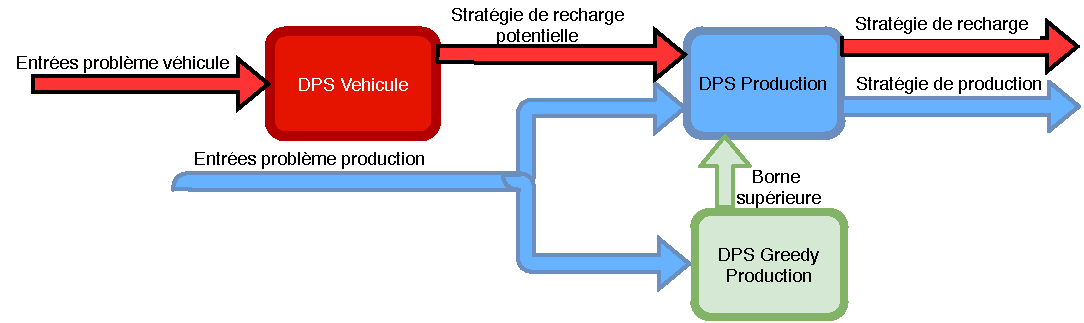
\includegraphics[height=4.5cm]{images_these/Pipeline.pdf}}
	\caption[Schéma du Pipe-line VD\_PM]{Schéma du Pipe-line VD\_PM.}
	\label{Pipeline}
\end{figure}

La décomposition \textbf{Pipe-line VD\_PM} (Voir figure (\ref{Pipeline})) suggère que la façon la plus simple de mettre en place une collaboration entre le conducteur du véhicule et le directeur de production est de les faire communiquer par le biais d'un pipeline à sens unique : une fois que le coefficient $\beta$  ait été fixé. $\beta$ détermine la fonction objectif du problème \textbf{VD} et se comporte comme le principal lien de communication entre le problème \textbf{VD} et le problème \textbf{PM}. La décomposition Pipe-line VD\_PM fonctionne de la facon suivante : on calcule d'abord une stratégie de recharge optimale en carburant $(x, L)$ pour le véhicule au moyen de l'algorithme \textbf{DPS\_VD}, on transforme ensuite cette stratégie $(x, L)$ en une stratégie de recharge réduite $(Q, \mu, m, M, B)$ et enfin on applique l'algorithme \textbf{DPS\_PM} sur cette stratégie de recharge réduite.  

\begin{Rem}
	Nous faisons communiquer un DPS fonctionnant en Backward (DPS\_VD) et un DPS fonctionnant en Forward (DPS\_PM) car dans la littérature ces deux schémas communiquent \og bien \fg{}.
\end{Rem}
Concernant les données d'entrées, nous supposons que nous recevons toutes les données relatives à la micro-usine et au véhicule, ainsi que le coefficient $\alpha$. Concernant la sortie désigné ici par \textbf{solution complète}, elle est constituée par le vecteur de production $z = (z_i, i = 0, \dots, N-1)$, le vecteur d'activation $y = (y_i, i = 0, \dots, N-1)$, le vecteur de recharge du véhicule $\delta= (\delta_i, i = 0, \dots, N-1)$, le vecteur de recharge du véhicule $x = (x_j, j = 0, \dots, M)$, le vecteur temps $T = (T_j, j = 0, \dots, M+1)$, le vecteur de la quantité rechargée $L = (L_j, j = 0, \dots, M)$, qui nous indique, dans le cas où $x_j = 1$, quelle quantité d'hydrogène est rechargée et la valeur $VAL$.
% $= \sum_{i = 0, \dots, N -1} (Cost^F\times y_i + Cost^V_i\times z_i) + \alpha \times T_{M+1}$ . 

Nous voyons ensuite que \textbf{SMEPC} peut être reformulée de manière collaborative comme suit : $\{$Fixez les coefficients et calculez une \textbf{stratégie de recharge optimale} $(x, L)$ de manière à ce que la \textit{stratégie de recharge réduite} $(Q, m, M, B, \mu)$ donne une stratégie de production $(z,\delta )$ avec un coût minimal de $\alpha \times p\times i_Q + \sum_{i = 0, \dots, N -1} (Cost^F\times y_i + Cost^V_i \times z_i)\}$.

\begin{algorithm} 
	\caption{Pipe-line VD\_PM}
	\label{VD-PM-Pipe-line}
	\begin{algorithmic}[1]
		\REQUIRE $N$, $M$, $TMax$ $H_0$, $E_0$, $C^{Tank}$, $C^{Veh}$,
		\ENSURE $Current\_Sol$, $Current\_Value$
		\hline
		
		\vspace{0.3cm}
		
		\STATE Fixer le coefficient $\beta$ du modèle \textbf{VD} ; 
		\STATE Appliquez le \textbf{DPS\_VD} au modèle \textbf{VD} et obtenez la \textbf{stratégie de recharge optimale} $(x, L)$ et récupérez la \textbf{stratégie de recharge réduite} $(Q,\mu , m, M, B)$ comme dans la section IV.3 ;
		\STATE Calculer $W^{Prod}_{Curr}$ par le biais de l'algorithme \textbf{Greedy\_PM} ;
		\STATE Résolvez l'instance de production par le biais de l'algorithme \textbf{Filtered\_DPS\_PM} à l'aide de la \textbf{stratégie de recharge réduite} $(Q,\mu , m, M, B)$ et de la \textbf{stratégie de recharge optimale} $(x, L)$;
		\STATE \textbf{Reconstruire la solution complète} en récupérant le vecteur d'activation $y = (y_i, i = 0, \dots, N-1 )$, le vecteur temps $T = (T_j, j = 0, \dots, M+1 )$, le vecteur de charge $L = (L_i, i = 0, \dots, N-1 )$, et le coût global $\alpha \times p\times i_Q + \sum_{i = 0, \dots, N -1} (Cost^F\times y_i + Cost^V_i \times z_i)\}$ ;
	\end{algorithmic}
\end{algorithm}

Les étapes de l'heuristique Pipe-line VD\_PM (Voir algorithme \ref{VD-PM-Pipe-line}) sont : 
\begin{enumerate}
	
	\item \underline{\textbf{Etape 1 :}} Fixer le coefficient $\beta$ ; 
	\item \underline{\textbf{Etape 2 :}} Résoudre, par le biais de l'algorithme \textbf{DPS\_VD}, l'instance du véhicule liée aux coefficients $\beta$ et $\alpha$ et obtenir le nombre d'opérations de recharge $Q$ ainsi que les vecteurs $m$, $M$ et $B$ ; 
	\item \underline{\textbf{Etape 3 :}} Calculer $W^{Prod}_{Curr}$ ainsi qu'une solution initiale $DEC\_PROD$ de l'instance de production liée à $\lambda= \alpha \times p$, par le biais de l'algorithme \textbf{Greedy\_PM} ;
	\item \underline{\textbf{Etape 4 :}} Résolvez l'instance de production résultante liée à $\lambda= \alpha \times p$, par le biais de l'algorithme \textbf{Filtered\_DPS\_PM} ;
	\item \underline{\textbf{Etape 5 :}} \textbf{Reconstruire la solution complète} du problème \textbf{SMEPC} (à la fois la tournée du véhicule et l'activité de la micro-usine), ainsi que sa valeur $VAL$. 
\end{enumerate}
Le choix de $\lambda$ vient de manière très naturelle : nous fixons $\lambda = \alpha \times p$. 
Nous devons d'abord préciser l'étape 5 : L'étape 2 nous a fourni une stratégie de recharge primaire, et donc les vecteurs $L$ et $ x$. Elle nous a également fourni le nombre $Q$ d'opérations de recharge, et, à l'aide de l'état FINAL et des composantes $Pred$ et $DEC$, nous dérivons de l'étape 4 les vecteurs $z$, $y$ et $\delta$. Afin d'obtenir le vecteur temps $T$, nous exécutons l'algorithme (	\ref{T-Reconstruction}).
\begin{algorithm}
	\caption{T\_Reconstruction}
	\label{T-Reconstruction}
	\begin{algorithmic}[1]
		\REQUIRE $M$, $t$, $d^*$, $p$, $\delta$
		\ENSURE $T$
		\hline
		\vspace{0.5cm}
		
		\INITIALISATION
		\STATE $T_0 \leftarrow 0$ ; $i\_aux \leftarrow 0$ ;
		
		\vspace{0.3cm}
		
		\BOUCLEPRINCIPAL
		\FOR{$j = 0$ \TO $M$ }
		\IF{$x_j=0$}
		\STATE $ T_{j+1} \leftarrow T_j + t_j$ ;
		\ELSE
		\STATE Calculer le plus petit $i_0 \geq i\_aux$ tel que $\delta_{i0}=1$ ;
		\STATE $T_{j+1} \leftarrow p \times (i_0+1)+d^*_{j+1}$ ;
		\STATE $i\_aux \leftarrow i_0+1$ ;
		\ENDIF
		\ENDFOR
	\end{algorithmic}
\end{algorithm}

Ensuite, la valeur $VAL$ est calculée d'une manière simple : 

$VAL=\alpha \times p\times [i_Q + d^*_{St_Q+1}+\sum_{j=St_Q+1, \dots, M-1}t_j + d_M] + \sum_{i = 0, \dots, N -1} (Cost^F\times y_i + Cost^V_i \times z_i)$.


Nous devons discuter de la manière de choisir $\beta$ car il doit refléter le coût de production de la quantité d'hydrogène $\sum_q \mu_q$ qui doit être produite pour permettre à la tournée augmentée $\Gamma(\beta)$ d'être effectuée. 
Cependant, nous n'avons aucune idée de ce que sera réellement ce coût, puisque nous ne connaissons pas a priori la répartition dans le temps de la manière dont cette énergie sera produite et consommée.

Nous pouvons utiliser les informations contenues dans le tableau $CostMin$, ainsi que dans le tableau $STATE^E$, en appliquant par exemple la formule suivante :
\begin{itemize}[label=$\square$]
	
	\item Soit $ H = STATE^E_{0, E_0} $; 
	\item $Rough\_Cost = CostMin(0, H/3 , 0) + CostMin( \left\lfloor N/3\right\rfloor, H/3 , 0) + CostMin(\left\lfloor 2N/3\right\rfloor, H/3 , 0)$ ;
	\item $\beta =Rough\_Cost / H$.
\end{itemize} 
Cette formule est une sorte d'estimation statistique du coût énergétique par unité qu'il faut accepter pour que le véhicule puisse effectuer sa tournée. 


%Paramétrage du modèle}
\section{Expérimentations numériques}
\label{Expe_VD_PM}
\subsection{Objectifs et contexte technique}
Notre objectif est d'évaluer :
\begin{enumerate} 
	\item Le schéma \textbf{Pipe-line VD\_PM} : nous nous concentrons sur le compromis induit par ce schéma entre la précision (gap par rapport à l'optimalité) et le temps d'exécution (résumé par le nombre d'états générés tout au long du processus). 
	\item La puissance de la valeur du \textbf{Pipe-line VD\_PM} comme borne supérieur pour l'algorithme général DPS\_SMEPC décrits au chapitre \ref{SMEPC_programmation}. Nous nous concentrons ici sur le nombre d'états générés au cours du processus en fonction des dispositifs de filtrage qui sont activés.
\end{enumerate}

Les algorithmes ont été implémentés en C++ et l'IDE utilisé est Visual Studio 2017. Les expérimentations sont réalisées sur un ordinateur équipé d'un processeur AMD EPYC 7H12 64-Core, 512 Go de RAM et
fonctionnent sous Gnu/linux Ubuntu 20.04.2. Le temps maximum du CPU est fixé à 1 heure.

%Les algorithmes ont été implémentés en C++, sur un ordinateur fonctionnant sous le système d'exploitation Windows 10 avec un processeur IntelCore i5-6500@3.20 GHz, 16 Go de RAM et le compilateur Visual Studio 2017.

%	\subsection{Procédés de génération d'instances du SMEPC}
%	\subsubsection{Génération aléatoire}
%	 Nous fixons $N$ et$ M$, et générons aléatoirement les stations $j$ et $Dépôt$ et la Micro-usine comme point de l'espace $\mathbb{R}^2$. Puis $d_j$, $d^*_j$, $t_j$, $e_j$, $\varepsilon_j$ et $\varepsilon^*_j$ correspondent respectivement à la distance euclidienne et à la distance de Manhattan, arrondies de telle sorte qu'elles prennent des valeurs intégrales. Ensuite, nous fixons $C^{Tank}$, $C^{Veh}$ et $TMax$, de telle sorte que cela assure l'existence d'une solution réalisable. Enfin, nous fixons les coefficients de coût, de telle sorte que le coût fixe $Cost^F$ soit au moins égal au plus grand coefficient $Cost^V_i, i = 0,\dots, N - 1$. 

\subsection{Instances}
Ici, nous utilisons un ensemble de 50 instances, avec les caractéristiques décrites par les tableaux (\ref{tab:inst2}) et (\ref{tab:inst}).

Pour les instances A et B illustrées respectivement aux figures (\ref{Inst_0}) et (\ref{Inst_1}), on a illustré les solutions obtenues par l'algorithme \textbf{Pipe-line VD\_PM}. Les solutions des instances A et B sont respectivement illustrées par les figures (\ref{Pipe_S_Inst_0}) et (\ref{Pipe_S_Inst_1}).


\begin{figure}[H]
	\centerline{
		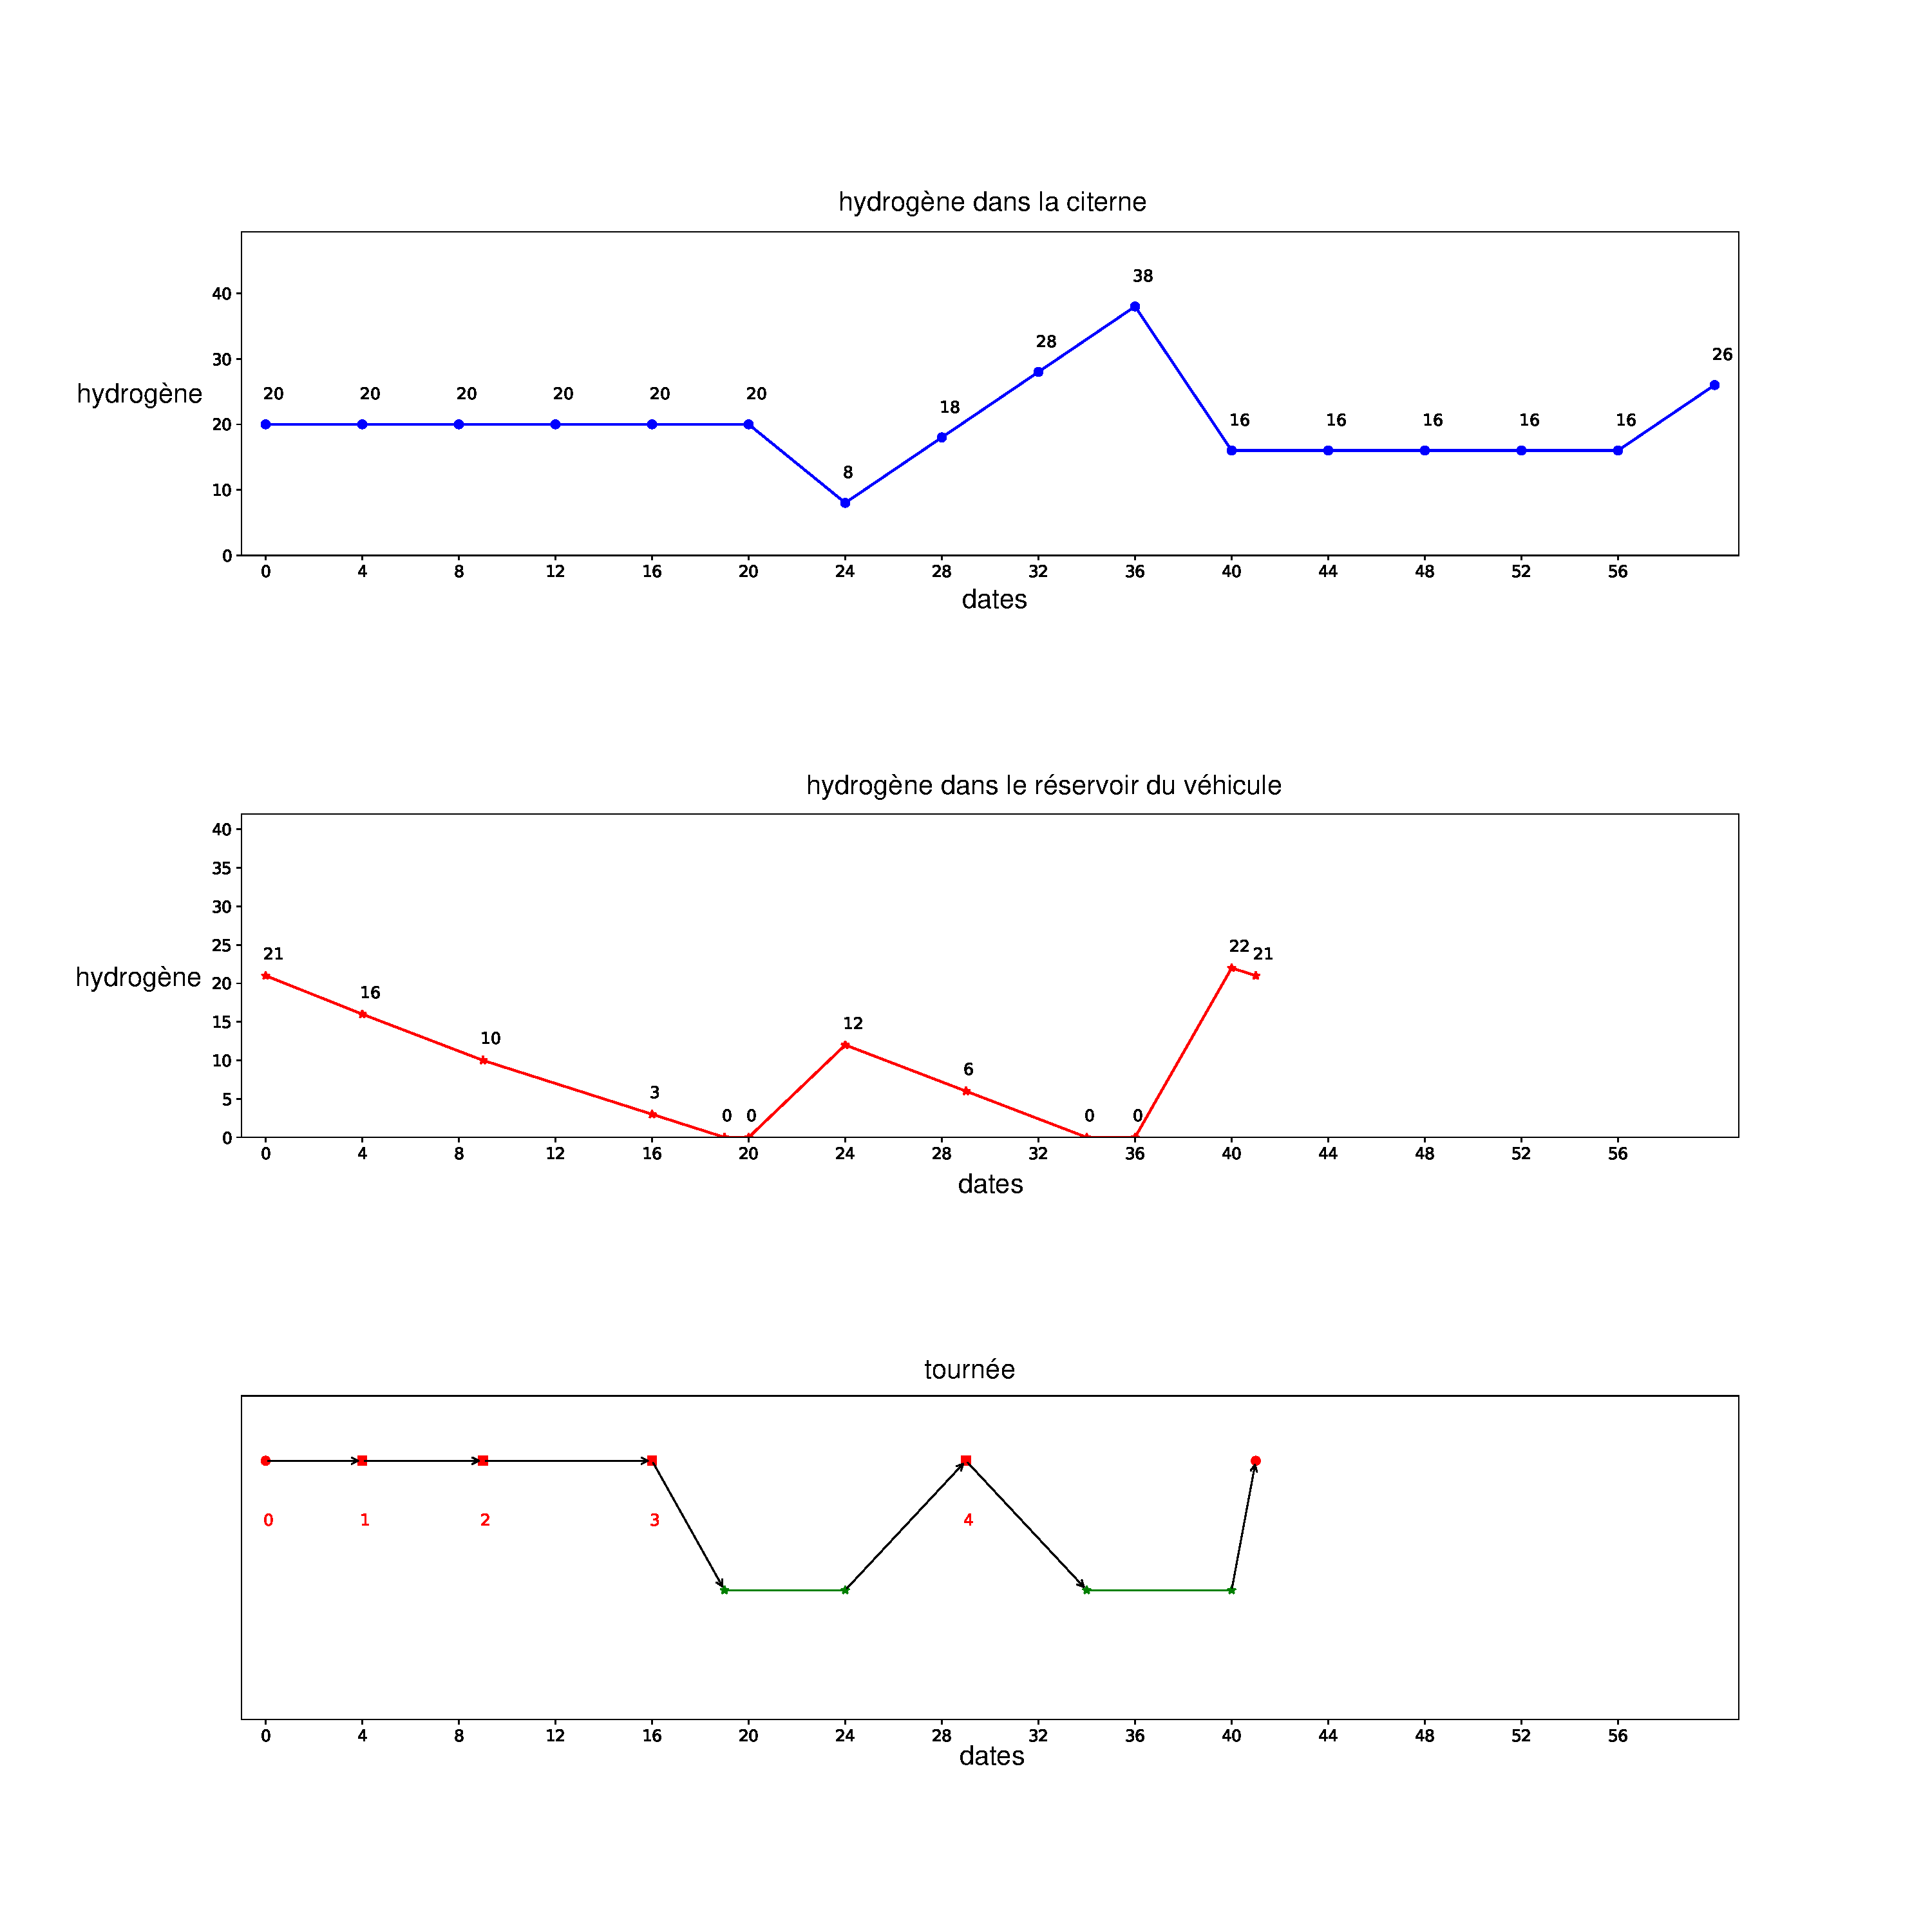
\includegraphics[height=20cm]{images_these/Pipe_sol_0.pdf}}
	\caption[La solution de l'instance A]{Solution de l'instance A : on a deux recharges, l'une entre la station 3 et la station 4 et l'autre entre la station 4 et le dépôt final.}
	\label{Pipe_S_Inst_0}
\end{figure}

\begin{figure}[H]
	\centerline{
		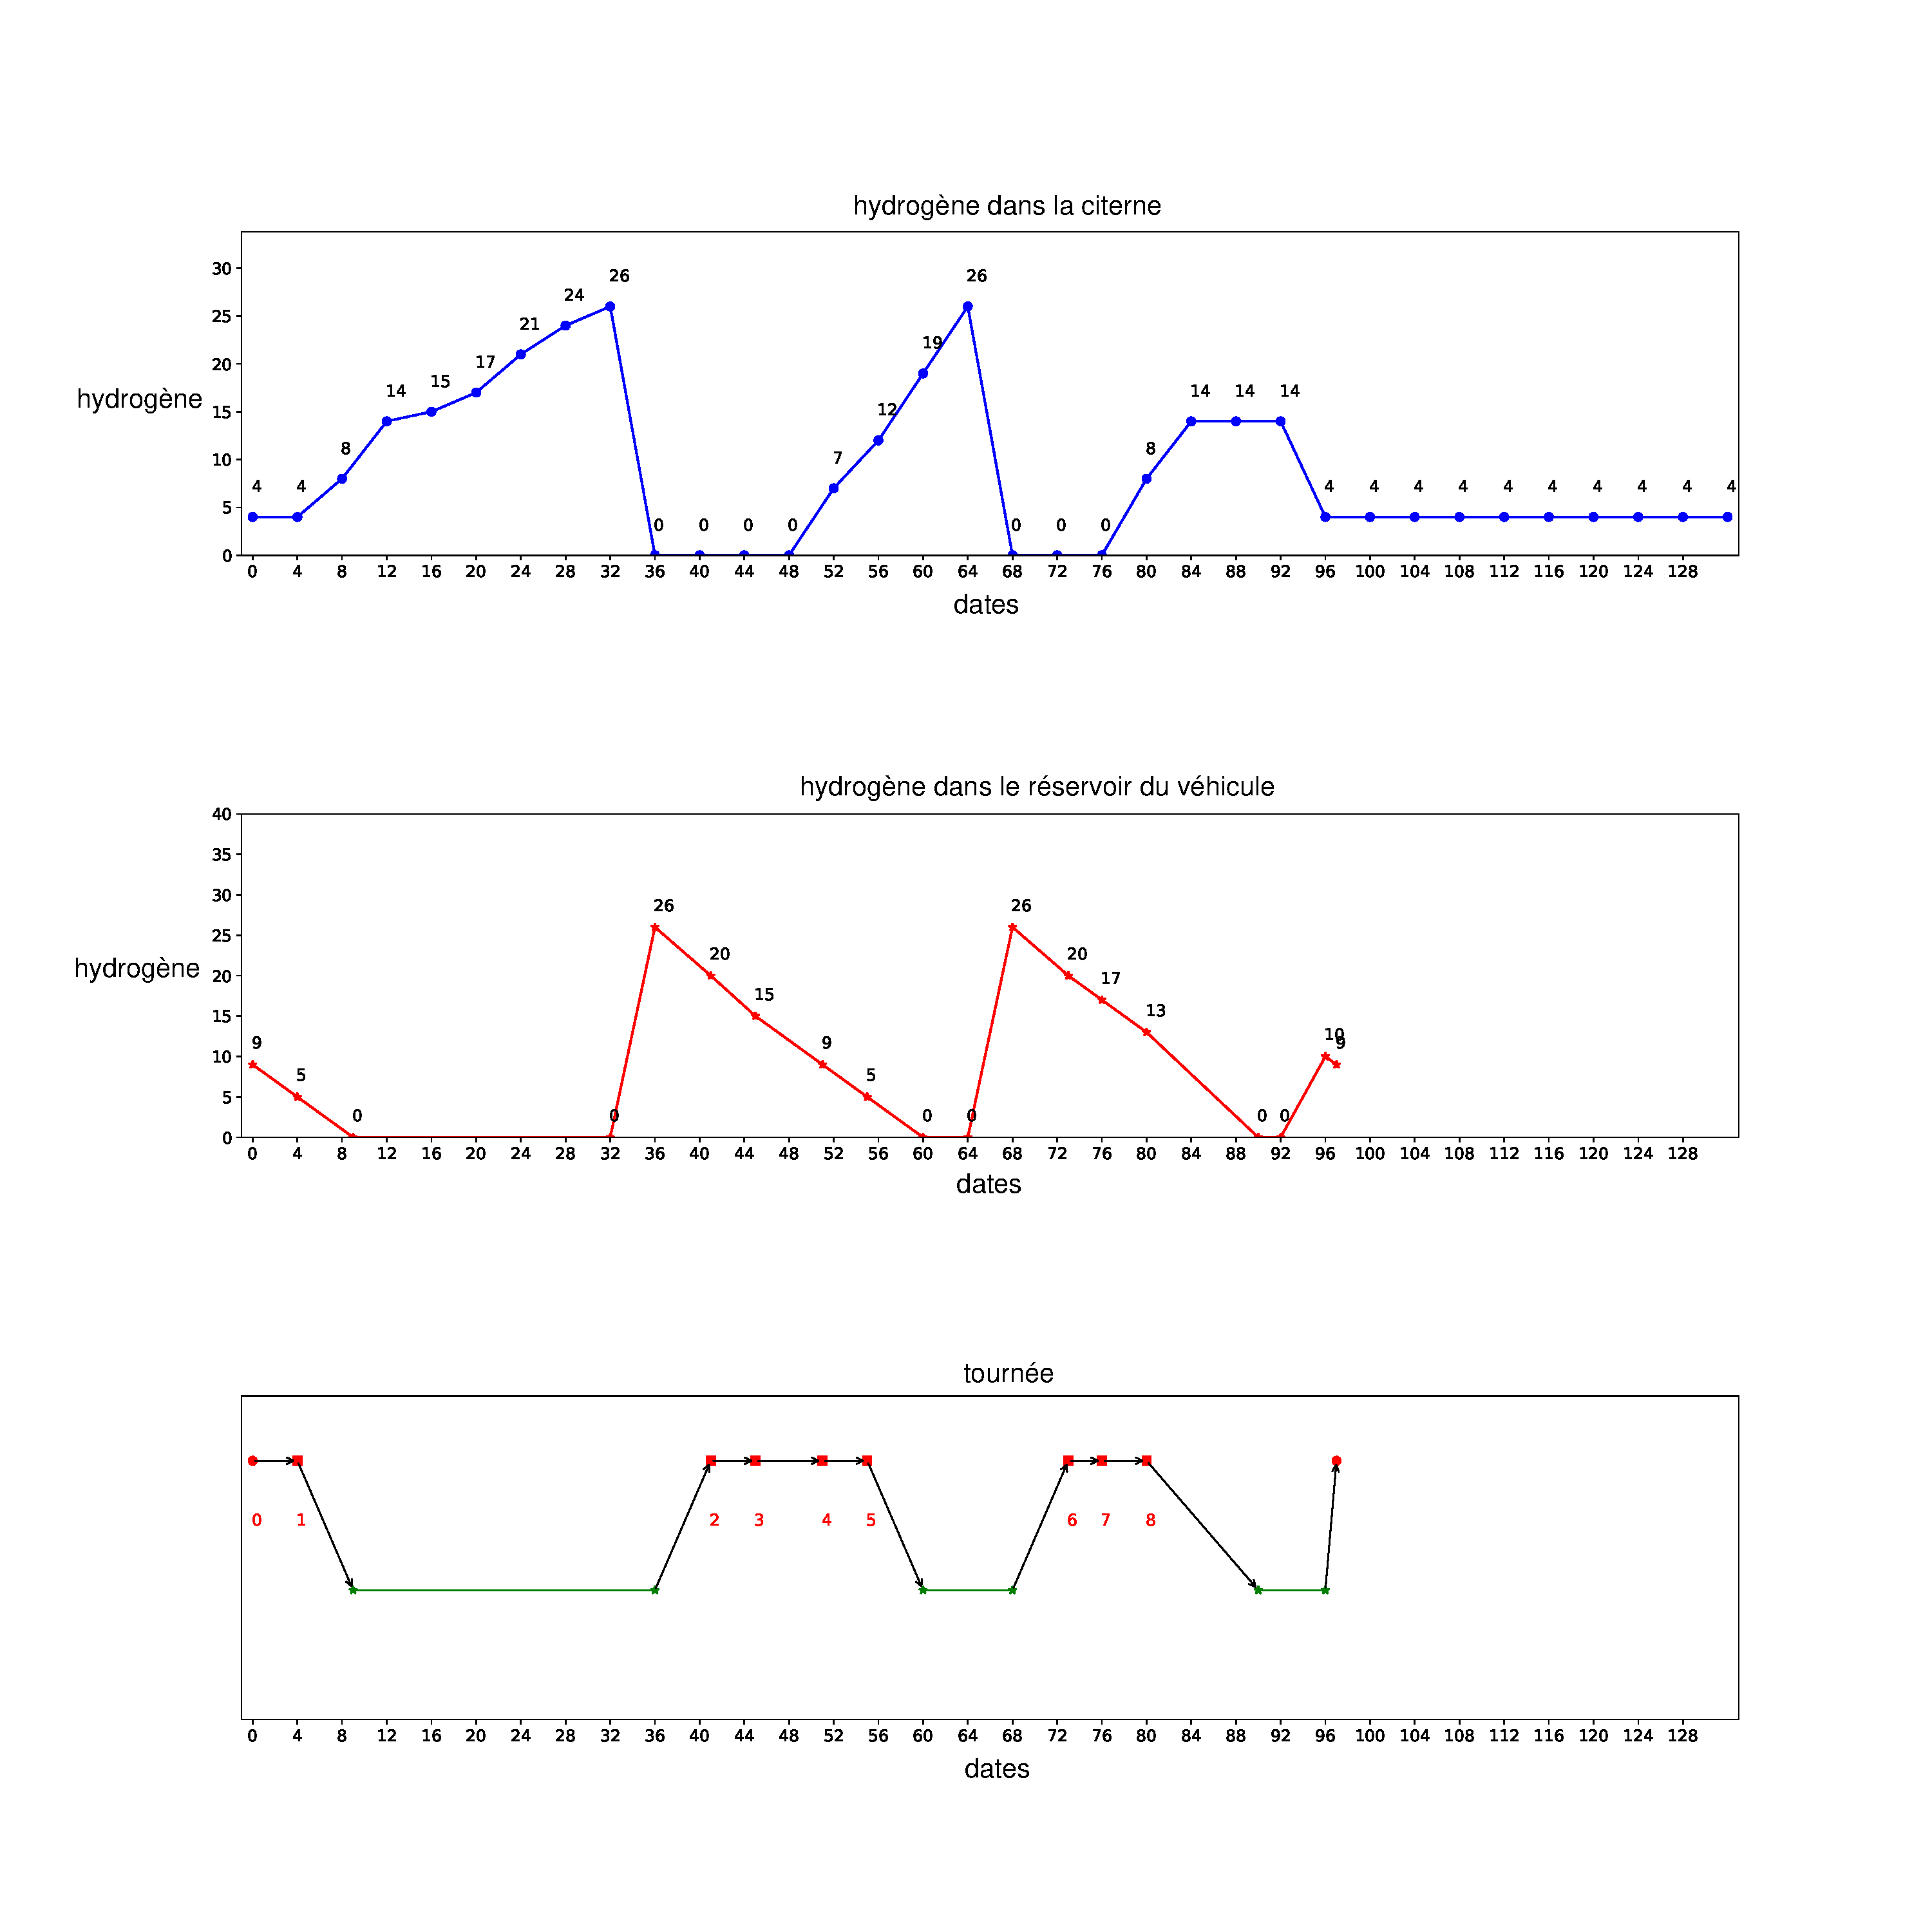
\includegraphics[height=20cm]{images_these/Pipe_sol_24.pdf}}
	\caption[La solution de l'instance B]{Solution de l'instance B : on a trois recharges.}
	\label{Pipe_S_Inst_1}
\end{figure}

\subsection{Comparaison de l'heuristique Pipe-line VD\_PM et du DPS\_SMEPC}
%Afin d'évaluer le schéma Pipe-line VD\_PM, nous lançons d'abord, pour chaque instance, l'exécution de \textbf{Greedy\_SMEPC} en sélectionnant 50 états à chaque étape , et obtenons une valeur $GS(50)$. Ensuite, nous exécutons \textbf{Pipe-line VD\_PM} et obtenons une valeur noté \textbf{Pipe-line}.  Enfin, nous lançons \textbf{DPS\_SMEPC} et obtenons une valeur \textbf{DPS\_SMEPC} optimale et exacte en utilisant comme BSUP la valeur $GS(50)$.  Nous obtenons donc les résultats suivants :
Similairement à ce qui a été fait au chapitre précédent, on exécute l'algorithme \textbf{Pipe-line VD\_PM} de quatre manières : 
\begin{enumerate}
	
	\item Sans mécanisme de filtrage, on nomme ces résultats $Pi(1)$ ;
	\item Avec les mécanismes de filtrage logique, on nomme ces résultats $Pi(2)$ ;
	\item Avec les mécanismes de filtrage logique et les mécanismes de filtrage par estimation optimiste, on nomme ces résultats $Pi(3)$ ;
	\item Avec les mécanismes de filtrage logique, les mécanismes de filtrage par estimation optimiste et  les mécanismes de filtrage heuristique, on nomme ces résultats $Pi(0)$. Concernant le filtrage heuristique, on a testé plusieurs valeurs de $K$ et on a choisi la plus petite valeur qui permettait d'avoir une solution de chaque instance. Le paramètre obtenu pour ces instances est $K=3$.
	
\end{enumerate}
Les tableaux de résultats ont la signification suivante :
\begin{itemize}[label=$\square$]
	
	\item Les tableaux (\ref{Comparaison_DPS-SMEPC_greed22}) et (\ref{Comparaison_DPS-SMEPC_greed}) contiennent les gaps par rapport à l'optimalité et le temps CPU des algorithmes respectivement pour les paquets d'instances INST\_CTE et INST\_VAR.
	La signification des colonnes est :
	\begin{itemize}
		\item  \textbf{Obj} est la valeur obtenue ;
		\item \textbf{Gap} est le gap par rapport à l'optimalité $Gap  = 100 \times \frac{Obj-opt}{opt}$ ; où $Obj$ est la valeur obtenue et $opt$ est la valeur optimale obtenue à l'aide du modèle $MILP_{SMEPC}$. Si une instance n'a pas été résolu jusqu'à l'optimalité, on utilise la borne supérieure de l'exécution sur 8 threads avec un temps limite de 3 heures (voir tableau (\ref{tab:resultSYM_STC}) et (\ref{tab:resultSYM_STC2})). %et de l'algorithme DPS\_SMEPC des deux chapitres précédents.
		\item \textbf{CPU} est le temps d'exécution en secondes. 
	\end{itemize}
	\item Les tableaux (\ref{Comparaison_nombre_state2}) et (\ref{Comparaison_nombre_state}) présentent les résultats respectivement pour les paquets d'instances INST\_CTE et INST\_VAR. Les tableaux (\ref{Comparaison_nombre_state2}) et (\ref{Comparaison_nombre_state}) contiennent le nombre maximal d'états $Re$, $Pr$ et $\# Etats$, respectivement des algorithmes DPS\_VD, DPS\_PM et DPS\_SMEPC.
	
	  
	%\item Le tableau (\ref{Comparaison_tempsCPU}) contient 
	%\item Le tableau (\ref{Comparaison_DPS-SMEPC_pipeline}) contient les valeurs du \textbf{DPS\_SMEPC} DPS\_SMEPC, Pipe-line et le gap $GAP\_Pipe$ par rapport à l'optimalité;  la valeur -1 signifie que l'algorithme n'a fournit aucune solution faisable.
	%\item Le tableau (\ref{Comparaison_tempsCPU2}) contient le temps CPU CPU (BSUP NS 1), CPU (BSUP pipeline) et CPU (BSUP PL 1 sec) de l'algorithme DPS Global en changeant la borne supérieure. Pour CPU (BSUP NS 1), CPU (BSUP pipeline) et CPU (BSUP PL 1 sec)les bornes supérieures utilisées sont respectivement calculées par GS(1), DPS Pipe-line et \textit{$MILP_{SMEPC}$}. En imposant  une seconde comme temps d'exécution pour \textit{$MILP_{SMEPC}$}.
\end{itemize}

On cherche à obtenir une évaluation de la qualité des solutions des algorithmes Pipe-line VD\_PM et une évaluation de l'impact des mécanismes de filtrage. Pour cela, on exécute plusieurs fois l'algorithme \textbf{Pipe-line VD\_PM} en activant à chaque fois les filtrages qui nous intéressent. La borne supérieure est calculée par l'algorithme \ref{Search_BSUP} présenté à la section \ref{Borne_sup} du chapitre précédent.

Pour le paquet d'instances INST\_CTE et le paquet d'instances INST\_VAR, on fait la remarque suivante : similairement au chapitre précédent, lorsqu'on ajoute les mécanismes de filtrage l'algorithme est de plus en plus rapide car les mécanismes de filtrage diminuent le nombre d'états. On constate qu'il n'y a pas diminution des gaps  lorsqu'on ajoute les mécanismes de filtrage logique.
On fait les remarques suivantes :
\begin{itemize}[label=$\square$]
	
	\item Comme pour le programme dynamique global, on a utilisé la même méthode de filtrage et les conclusions sont identiques. C'est-à-dire que l'ajout du filtrage heuristique est efficace. C'est majoritaire sur le paquet d'instances INST\_VAR qu'on voit l'efficace du filtrage heuristique (on a une amélioration des gaps et une diminution du temps d'exécution des instances du paquet INST\_VAR) ;
	\item  Concernant les instances du paquet INST\_CTE, l'algorithme Pipe-Line est plus rapide avec les filtrages heuristiques mais la qualité de la solution n'est pas impactée ; 
	
	\item  Le nombre d'états du paquet d'instances INST\_CTE est inférieur au nombre d'états du paquet d'instances INST\_VAR ;
	\item  Le nombre d'états du Pipe-Line est inférieur à celui du programme dynamique ;
	\item  Le gap  et le temps CPU de l'heuristique Pipe-Line sont de moins bonne qualité que ceux de l'algorithme DPS\_SMEPC avec tous les filtrages. Mais par contre le Pipe-Line réussit à résoudre certaines instances que le DPS\_SMEPC avec les filtrages exactes ne parvient pas à résoudre.
\end{itemize}
\subsubsection{Comparaison de l'heuristique Pipe-line VD\_PM et du DPS\_SMEPC : les instances du paquet INST\_VAR}
Les tableaux (\ref{Comparaison_DPS-SMEPC_greed22}) et (\ref{Comparaison_nombre_state2}) présentent les résultats des instances du paquet INST\_VAR. 
%On cherche à obtenir une évaluation de la qualité des solutions des algorithmes Pipe-line VD\_PM et une évaluation de l'impact des mécanismes de filtrage. Pour cela, on exécute plusieurs fois l'algorithme \textbf{Pipe-line VD\_PM} en activant à chaque fois les filtrages qui nous intéressent. La borne supérieure est celle obtenue à la section \ref{Borne_sup}. 
Lorsque la valeur vaut \og - \fg{} cela veut dire que l'algorithme s'est arrêté au bout d'une heure sans trouver de solution. 


\textbf{Comparaison des gaps et du temps CPU des instances du paquet INST\_VAR :}

Le tableau (\ref{Comparaison_DPS-SMEPC_greed22}) présente la comparaison des gaps et du temps de calcul (CPU) en secondes obtenus par l'exécution des algorithmes Pipe-line VD\_PM sur les instances du paquet INST\_VAR.
En analysant les résultats des instances du paquet INST\_VAR, on remarque que le filtrage heuristique est efficace car on obtient toujours une solution en moins d'une heure. Or, $Pi(1)$, $Pi(2)$ et $Pi(3)$ ne parvient pas à résoudre en moyenne 47,7\% des instances en moins d'une heure. De plus, en ajoutant le filtrage heuristique la méthode devient très rapide et on obtient des gaps qui sont inférieurs à 7\%, ce filtrage ne dégrade que légèrement la solution. De plus, avec le filtrage heuristique, on obtient 6 solutions optimales en moins de 0,01 seconde. Par exemple, pour l'instance 36, on passe de 28,8 minutes de temps d'exécution lorsqu'on exécute sans filtrage à 0,68 seconde lorsqu'on exécute avec tous les filtrages et on a un gap de 0,54\%.
Globalement le gap moyen des colonnes Pi(0), Pi(3), Pi(2), Pi(1) est respectivement 1,21 ; 1,21 ; 2,31 ; 2,31 et le temps d'exécution moyen en seconde est respectivement 210,78 ; 1665,32 ; 1887,92 ; 1924,61.  
On a calculé la moyenne des gaps seulement sur les 11 premiers instances. 
%La valeur moyenne de Pi(0), Pi(3), Pi(2), Pi(1) est respectivement 1488,133 ; 557,033 ; 309,033; 1924,613.
 %On constate qu'il y a diminution du gap uniquement lorsqu'on ajoute le filtrage par estimation optimiste (basée sur la borne supérieure).
% On remarque que lorsqu'on ajoute des mécanismes de filtrage l'algorithme est de plus en plus rapide car les mécanismes de filtrage diminuent le nombre d'états. 
%%%%%%%%%%%%%%%%%%%%%%%%%%%%%%%%%%%%%%%%%%%%%%%%%%%%%%%%%%%%%%%%%%%%%%%%%%%%%%%%%%%%%%%%%
\begin{table}[H]
	\centering
	\small
	\begin{tabular}{|r|rrr|rrr|rrr|rrr|}
		\toprule
		\hline
		\rowcolor{cyan}	& \multicolumn{3}{c|}{\textbf{Pi(0)}}&\multicolumn{3}{c|}{\textbf{Pi(3)}}&\multicolumn{3}{c|}{\textbf{Pi(2)}}&\multicolumn{3}{c|}{\textbf{Pi(1)}} \\ \hline
		\midrule
		
			\hline
		\rowcolor{cyan}	&\multicolumn{3}{c|}{ \tiny{Tous les filtrages exacts et heuristiques}} & \multicolumn{3}{c|}{\tiny{Tous les filtrages exacts}}&\multicolumn{3}{c|}{\tiny{Filtrages logiques et optimistes}}&\multicolumn{3}{c|}{\tiny{Sans filtrage}}
		\\ \hline
		\midrule
		
		\rowcolor{cyan}	\textbf{num} & \textbf{Obj}& \textbf{Gap}  & \textbf{CPU} & \textbf{Obj}& \textbf{Gap}  & \textbf{CPU} & \textbf{Obj}& \textbf{Gap}  & \textbf{CPU} & \textbf{Obj}&\textbf{Gap}  & \textbf{CPU} \\ \hline
		\midrule
	
1	&	131	&	0,00	&	0,00	&	131	&	0,00	&	0,00	&	131	&	0,00	&	0,00	&	131	&	0,00	&	0,00	\\ \hline
2	&	151	&	0,00	&	0,00	&	151	&	0,00	&	0,00	&	151	&	0,00	&	0,00	&	151	&	0,00	&	0,00	\\ \hline
3	&	144	&	0,00	&	0,00	&	144	&	0,00	&	0,00	&	154	&	6,94	&	0,22	&	154	&	6,94	&	0,22	\\ \hline
4	&	149	&	6,43	&	0,00	&	149	&	6,43	&	0,00	&	149	&	6,43	&	0,01	&	149	&	6,43	&	0,01	\\ \hline
5	&	161	&	0,00	&	0,00	&	161	&	0,00	&	0,00	&	161	&	0,00	&	0,34	&	161	&	0,00	&	0,35	\\ \hline
6	&	179	&	0,56	&	0,01	&	179	&	0,56	&	0,14	&	179	&	0,56	&	0,18	&	179	&	0,56	&	0,18	\\ \hline
7	&	222	&	0,00	&	0,00	&	222	&	0,00	&	0,00	&	222	&	0,00	&	0,00	&	222	&	0,00	&	0,00	\\ \hline
8	&	195	&	1,56	&	0,00	&	195	&	1,56	&	0,01	&	195	&	1,56	&	0,33	&	195	&	1,56	&	0,33	\\ \hline
9	&	644	&	0,00	&	0,00	&	644	&	0,00	&	5,70	&	644	&	0,00	&	34,15	&	644	&	0,00	&	34,69	\\ \hline
10	&	1142	&	0,26	&	0,00	&	1142	&	0,26	&	0,94	&	1142	&	0,26	&	1,91	&	1142	&	0,26	&	1,94	\\ \hline
11	&	140	&	4,48	&	0,00	&	140	&	4,48	&	0,00	&	147	&	9,70	&	0,84	&	147	&	9,70	&	0,84	\\ \hline
12	&	916	&	0,44	&	0,48	&	916	&	0,44	&	1670,67	&	-	&	-	&	3600,00	&	-	&	-	&	3600,00	\\ \hline
13	&	960	&	0,42	&	0,06	&	960	&	0,42	&	36,50	&	960	&	0,42	&	193,63	&	960	&	0,42	&	193,78	\\ \hline
14	&	1387	&	1,09	&	0,33	&	1387	&	1,09	&	3600,00	&	-	&	-	&	3600,00	&	-	&	-	&	3600,00	\\ \hline
15	&	1348	&	0,15	&	0,34	&	1348	&	0,15	&	67,34	&	1348	&	0,15	&	77,18	&	1348	&	0,15	&	78,36	\\ \hline
16	&	1298	&	0,54	&	0,68	&	1298	&	0,54	&	387,76	&	1298	&	0,54	&	1176,70	&	1298	&	0,54	&	1729,44	\\ \hline
17	&	1318	&	2,57	&	5,35	&	-	&	-	&	3600,00	&	-	&	-	&	3600,00	&	-	&	-	&	3600,00	\\ \hline
18	&	2390	&	0,72	&	0,84	&	2390	&	0,72	&	381,34	&	2390	&	0,72	&	1152,14	&	2390	&	0,72	&	1698,25	\\ \hline
19	&	2306	&	4,20	&	67,40	&	-	&	-	&	3600,00	&	-	&	-	&	3600,00	&	-	&	-	&	3600,00	\\ \hline
20	&	2679	&	0,75	&	0,34	&	2679	&	0,75	&	609,14	&	-	&	-	&	3600,00	&	-	&	-	&	3600,00	\\ \hline
21	&	1496	&	6,10	&	63,50	&	-	&	-	&	3600,00	&	-	&	-	&	3600,00	&	-	&	-	&	3600,00	\\ \hline
22	&	1365	&	1,71	&	63,40	&	-	&	-	&	3600,00	&	-	&	-	&	3600,00	&	-	&	-	&	3600,00	\\ \hline
23	&	2743	&	5,91	&	281,64	&	-	&	-	&	3600,00	&	-	&	-	&	3600,00	&	-	&	-	&	3600,00	\\ \hline
24	&	2943	&	4,92	&	88,85	&	-	&	-	&	3600,00	&	-	&	-	&	3600,00	&	-	&	-	&	3600,00	\\ \hline
25	&	2124	&	3,46	&	4,11	&	-	&	-	&	3600,00	&	-	&	-	&	3600,00	&	-	&	-	&	3600,00	\\ \hline
26	&	2376	&	0,85	&	4489,96	&	-	&	-	&	3600,00	&	-	&	-	&	3600,00	&	-	&	-	&	3600,00	\\ \hline
27	&	2475	&	0,28	&	0,43	&	2475	&	0,28	&	3600,01	&	-	&	-	&	3600,00	&	-	&	-	&	3600,00	\\ \hline
28	&	3138	&	2,75	&	415,68	&	-	&	-	&	3600,00	&	-	&	-	&	3600,00	&	-	&	-	&	3600,00	\\ \hline
29	&	4506	&	1,56	&	780,54	&	-	&	-	&	3600,00	&	-	&	-	&	3600,00	&	-	&	-	&	3600,00	\\ \hline
30	&	3618	&	2,73	&	59,33	&	-	&	-	&	3600,00	&	-	&	-	&	3600,00	&	-	&	-	&	3600,00	\\ \hline

		
		\bottomrule
	\end{tabular}%
	\caption{Les instances du paquet INST\_VAR : Comparaison des gaps et du temps CPU du Pipe-Line VD\_PM.}
	
	\label{Comparaison_DPS-SMEPC_greed22}%
\end{table}%
%%%%%%%%%%%%%%%%%%%%%%%%%%%%%%%%%%%%%%%%%%%%%%%%%%
\begin{figure}[H]
	\centering
	\begin{tabular}{c c}
		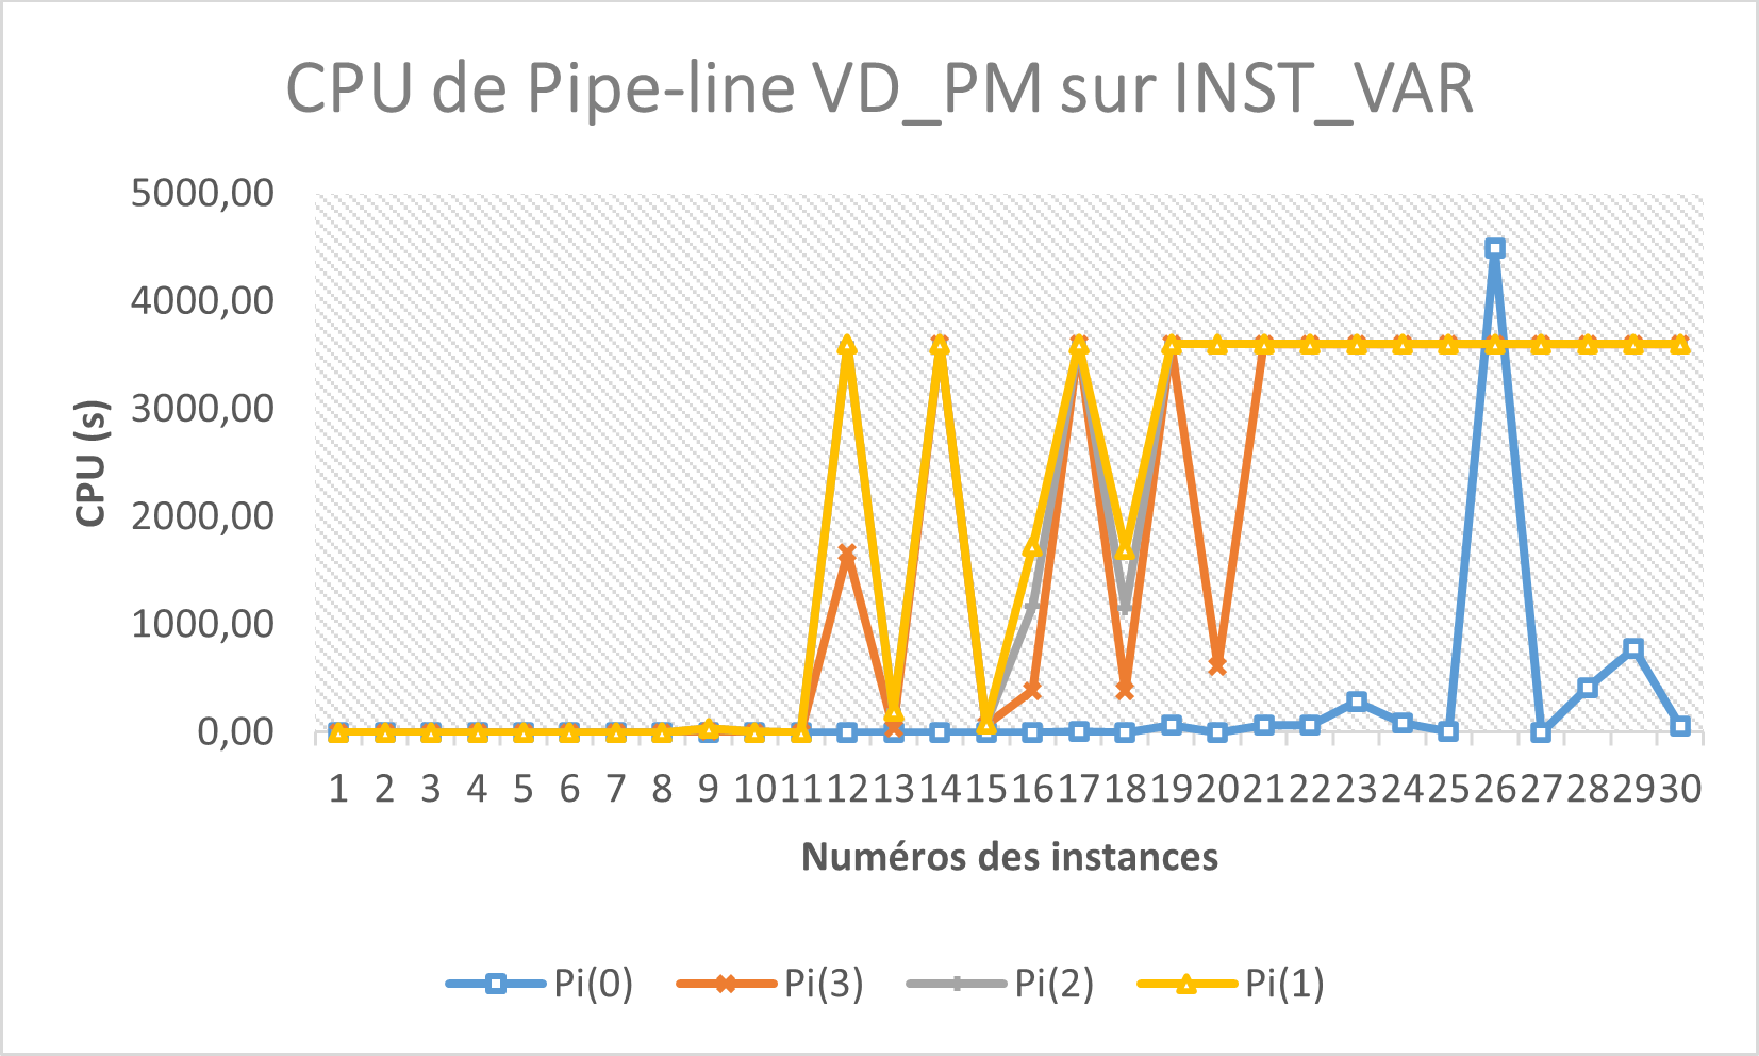
\includegraphics[width=9cm]{images_these/CPU_Pipe_INST_VAR.pdf}&
		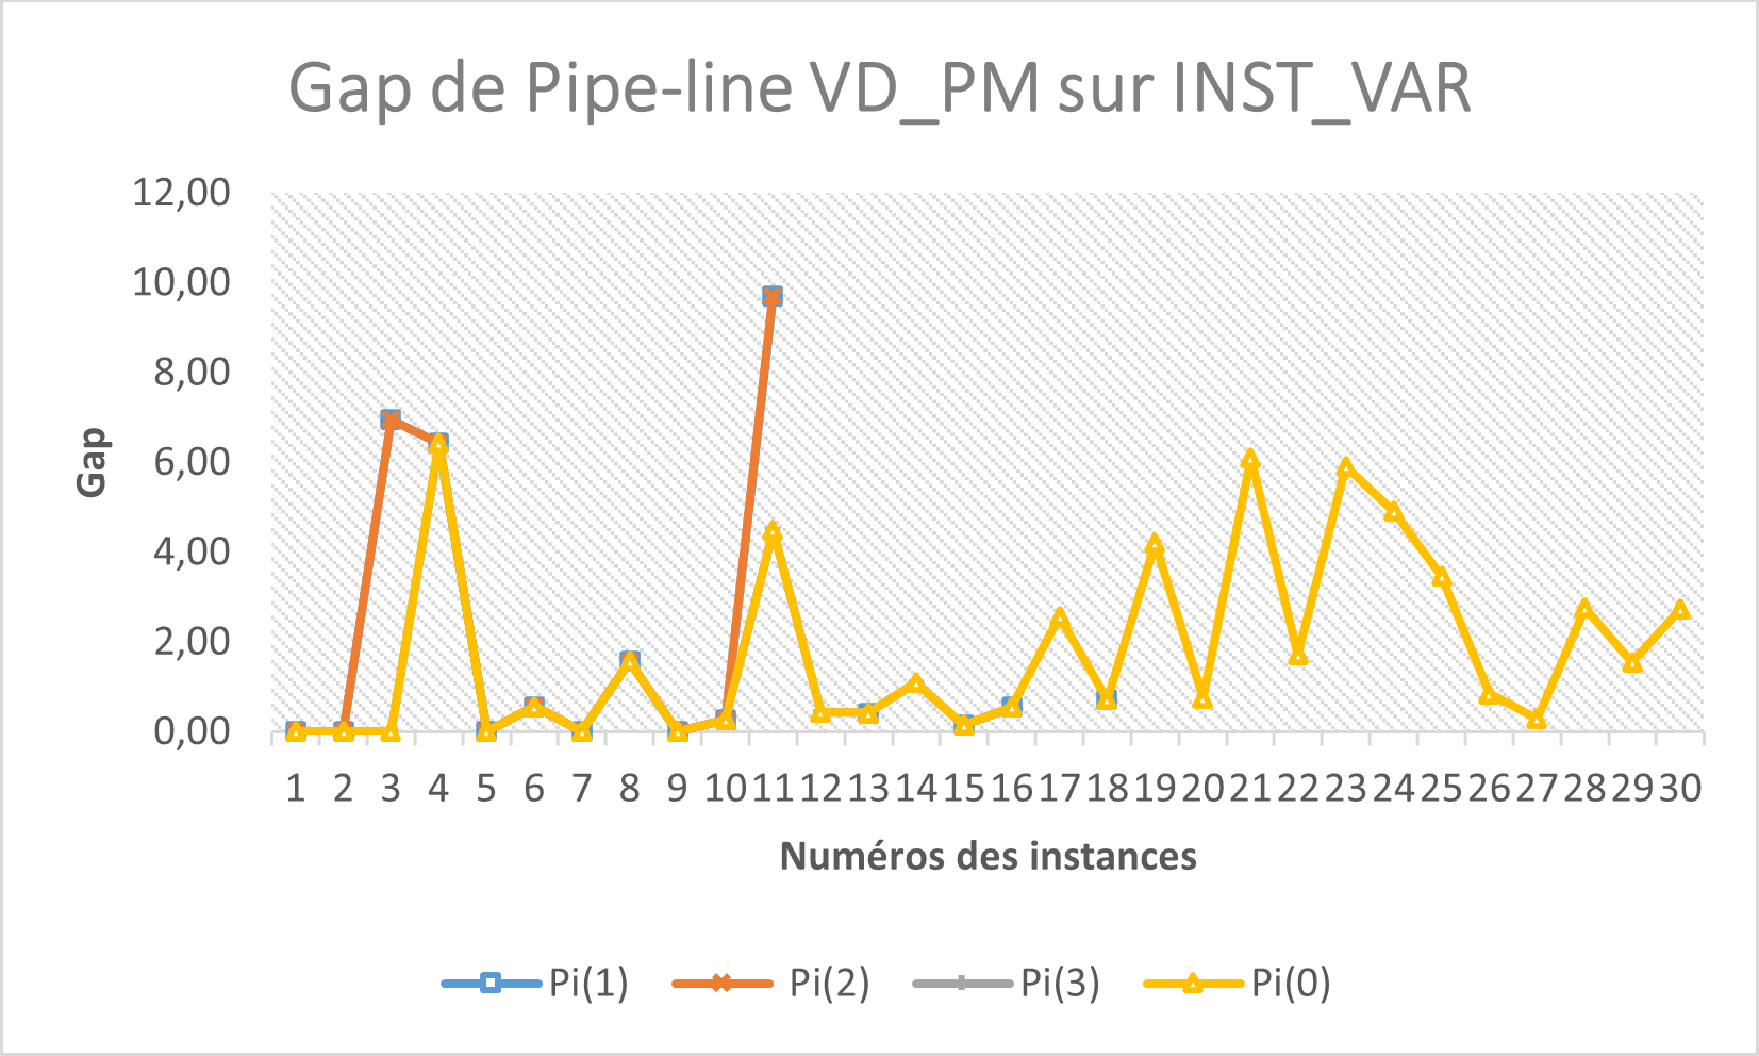
\includegraphics[width=9cm]{images_these/Gap_Pipe_INST_VAR.pdf}
		\\
		(a) & (b)
	\end{tabular}
	\caption[Représentation graphique du CPU et du gap du tableau (\ref{Comparaison_DPS-SMEPC_greed22})]{Représentation graphique du tableau (\ref{Comparaison_DPS-SMEPC_greed22}). (a) représente le temps CPU et (b) représente le gap de chaque instance de INST\_VAR.}\label{gap_cpu_pipe_INST_VAR}
\end{figure}

\textbf{Comparaison du nombre d'états générés des instances du paquet INST\_VAR :}

Le tableau (\ref{Comparaison_nombre_state2}) présente la comparaison du nombre d'états générés par le  Pipe-line VD\_PM et le DPS\_SMEPC pour les instances du paquet INST\_VAR. Le nombre maximal d'états est appelé $Re$, $Pr$ et $\# Etats$, respectivement pour les algorithmes DPS\_VD, DPS\_PM et DPS\_SMEPC. Le nombre d'états générés par l'algorithme DPS\_VD est inférieur au nombre d'états générés par l'algorithme DPS\_PM ce qui montre que le problème de production est le plus difficile des deux. Le nombre d'états générés par l'algorithme \textbf{DPS\_SMEPC} est supérieur au nombre d'états générés par l'algorithme Pipe-Line VD\_PM.
Globalement le nombre d'états moyen de Pi(0), Pi(3), Pi(2), Pi(1) est respectivement 
7703,667 ; 137301,267 ; 201852,033 ; 202426,6
et le nombre d'états moyen du DPS\_SMEPC est respectivement
 2449,133 ; 799762,733 ; 962697,333 ; 1033360,2. 
%On remarque que lorsqu'on ajoute des mécanismes de filtrage l'algorithme est de plus en plus rapide car les mécanismes de filtrage diminue le nombre d'états. En comparant le nombre d'états de chaque algorithme, on constante que le mécanisme de filtrage exact le plus efficace est le filtrage par estimation optimiste.

%%%%%%%%%%%%%%%%%%%%%%%%%%%%%%%%%%%%%%%%%%%%%%%%%%%%%%%%%%%%%%%%%%%%%%%%%%%%%%%%%%%%%%%%%
\begin{table}[H]
	\centering
	\small
	\begin{tabular}{|r|rrr|rrr|rrr|rrr|}
		\toprule
		\hline
		\rowcolor{cyan}	&\multicolumn{3}{c|}{\textbf{Pi(0)}} & \multicolumn{3}{c|}{\textbf{Pi(3)}}&\multicolumn{3}{c|}{\textbf{Pi(2)}}&\multicolumn{3}{c|}{\textbf{Pi(1)}} \\ \hline
		\midrule
		
			\hline
		\rowcolor{cyan}	&\multicolumn{3}{c|}{ \tiny{Tous les filtrages exacts et heuristiques}} & \multicolumn{3}{c|}{\tiny{Tous les filtrages exacts}}&\multicolumn{3}{c|}{\tiny{Filtrages logiques et optimistes}}&\multicolumn{3}{c|}{\tiny{Sans filtrage}}
		\\ \hline
		\midrule
		
		\rowcolor{cyan}	\textbf{num} & \textbf{Re} & \textbf{Pr} & \textbf{\#Etats} & \textbf{Re} & \textbf{Pr} & \textbf{\#Etats} & \textbf{Re} & \textbf{Pr} & \textbf{\#Etats} &\textbf{Re} & \textbf{Pr} & \textbf{\#Etats} \\ \hline
		\midrule
	1	&	3	&	42	&	61	&	3	&	78	&	554	&	3	&	669	&	4329	&	3	&	745	&	4604	\\ \hline
	2	&	3	&	84	&	161	&	3	&	381	&	1739	&	3	&	683	&	4241	&	3	&	683	&	4820	\\ \hline
	3	&	5	&	29	&	63	&	5	&	99	&	2213	&	5	&	5932	&	129720	&	5	&	5932	&	131744	\\ \hline
	4	&	3	&	142	&	321	&	3	&	748	&	2155	&	3	&	887	&	4748	&	3	&	887	&	4865	\\ \hline
	5	&	3	&	75	&	48	&	3	&	223	&	406	&	3	&	6880	&	82005	&	3	&	6880	&	83001	\\ \hline
	6	&	3	&	388	&	198	&	3	&	3142	&	9960	&	3	&	3275	&	13761	&	3	&	3275	&	19072	\\ \hline
	7	&	3	&	71	&	126	&	3	&	352	&	1732	&	3	&	531	&	7914	&	3	&	531	&	14375	\\ \hline
	8	&	3	&	160	&	87	&	3	&	1189	&	1607	&	3	&	6879	&	37060	&	3	&	6879	&	39376	\\ \hline
	9	&	4	&	200	&	286	&	4	&	15047	&	263867	&	4	&	33344	&	1410815	&	4	&	33344	&	1344462	\\ \hline
	10	&	3	&	128	&	148	&	3	&	8682	&	326094	&	3	&	10295	&	716815	&	3	&	10295	&	1024128	\\ \hline
	11	&	3	&	109	&	29	&	3	&	343	&	536	&	3	&	8681	&	42913	&	3	&	8681	&	43867	\\ \hline
	12	&	3	&	1343	&	314	&	3	&	167455	&	613249	&	3	&	292458	&	1020778	&	3	&	292458	&	1020778	\\ \hline
	13	&	4	&	575	&	59	&	4	&	34943	&	7115	&	4	&	75634	&	1610932	&	4	&	75634	&	1610932	\\ \hline
	14	&	3	&	990	&	642	&	3	&	191783	&	1550626	&	3	&	274485	&	1559487	&	3	&	314032	&	1559487	\\ \hline
	15	&	4	&	1485	&	106	&	4	&	46227	&	261078	&	4	&	48830	&	1067321	&	4	&	48830	&	1115578	\\ \hline
	16	&	5	&	1946	&	429	&	5	&	93550	&	909386	&	5	&	149187	&	1118045	&	5	&	149187	&	1118045	\\ \hline
	17	&	5	&	3264	&	410	&	5	&	223991	&	703595	&	5	&	279528	&	1019333	&	5	&	313384	&	1169832	\\ \hline
	18	&	5	&	1921	&	390	&	5	&	78975	&	872810	&	5	&	124484	&	764772	&	5	&	124484	&	1256433	\\ \hline
	19	&	4	&	10669	&	442	&	4	&	230526	&	2238483	&	4	&	349693	&	2010204	&	4	&	439033	&	2238483	\\ \hline
	20	&	6	&	1274	&	609	&	6	&	113612	&	1137757	&	6	&	379034	&	918477	&	6	&	379034	&	1227651	\\ \hline
	21	&	4	&	11650	&	2138	&	4	&	274431	&	1207299	&	4	&	352392	&	846485	&	4	&	352392	&	1219554	\\ \hline
	22	&	4	&	9253	&	5148	&	4	&	262745	&	1759894	&	4	&	347328	&	1687911	&	4	&	329060	&	1850181	\\ \hline
	23	&	4	&	21541	&	1284	&	4	&	321030	&	1320005	&	4	&	391639	&	1320005	&	4	&	374281	&	1320005	\\ \hline
	24	&	4	&	11074	&	1116	&	4	&	330588	&	1450961	&	4	&	386736	&	1450961	&	4	&	362386	&	1450961	\\ \hline
	25	&	8	&	1832	&	869	&	8	&	251611	&	1626287	&	8	&	417729	&	1484155	&	8	&	417729	&	1484155	\\ \hline
	26	&	6	&	94544	&	53759	&	6	&	197492	&	1550660	&	6	&	352015	&	1637832	&	6	&	352015	&	1637832	\\ \hline
	27	&	6	&	799	&	696	&	6	&	242065	&	1817157	&	6	&	433076	&	2510242	&	6	&	410623	&	2510242	\\ \hline
	28	&	4	&	18516	&	1258	&	4	&	309715	&	1468315	&	4	&	403883	&	1468854	&	4	&	388750	&	1468854	\\ \hline
	29	&	4	&	28811	&	1070	&	4	&	337806	&	1764386	&	4	&	428650	&	1764386	&	4	&	380630	&	1861070	\\ \hline
	30	&	8	&	8068	&	1207	&	8	&	380082	&	1122956	&	8	&	490597	&	1166419	&	8	&	490597	&	1166419	\\ \hline
		
		\bottomrule
	\end{tabular}%
	\caption{Les instances du paquet INST\_VAR : impact des mécanismes de filtrage.}
	
	\label{Comparaison_nombre_state2}%
\end{table}%
%%%%%%%%%%%%%%%%%%%%%%%%%%%%%%%%%%%%%%%%%%%%%%%%%%


\subsubsection{Comparaison de l'heuristique Pipe-line VD\_PM et du DPS\_SMEPC : les instances du paquet INST\_CTE}

Les tableaux (\ref{Comparaison_DPS-SMEPC_greed}) et (\ref{Comparaison_nombre_state}) présentent les résultats des instances du paquet INST\_CTE.% On cherche à obtenir une évaluation de la qualité des solutions des algorithmes Pipe-line VD\_PM et une évaluation de l'impact des mécanismes de filtrage. Pour cela, on exécute plusieurs fois l'algorithme \textbf{Pipe-line VD\_PM} en activant à chaque fois les filtrages qui nous intéressent. La borne supérieure est celle obtenue à la section \ref{Borne_sup}.


\textbf{Comparaison des gaps et du temps CPU des instances du paquet INST\_CTE :}

Similairement à la section précédente, le tableau (\ref{Comparaison_DPS-SMEPC_greed}) présente la comparaison des gaps et la comparaison du temps CPU en secondes obtenus lors de l'exécution des algorithmes Pipe-line VD\_PM sur les instances du paquet INST\_CTE.
En analysant les résultats des instances du paquet INST\_CTE, on remarque qu'avec le filtrage heuristique on obtient 50\% de solutions optimales très rapidement. 
On remarque que le temps d'exécution des algorithmes Pipe-Line VD\_PM est très rapide car il est toujours inférieur à 0,01 seconde. 
Concernant le gap, les filtrages sur les algorithmes Pipe-Line VD\_PM sont moins efficaces que sur le schéma général \textbf{DPS\_SMEPC}. Car on constate que pour 18 instances les gaps obtenus sans filtrage sont identiques à ceux avec filtrage. Par contre on remarque une amélioration du temps d'exécution.
Globalement, le gap moyen de Pi(0), Pi(3), Pi(2), Pi(1) est respectivement 2,253 ; 2,253 ; 3,767 ; 3,767 et le temps d'exécution moyen en seconde est respectivement 0,00005 ; 0,00145 ; 0,04955 ; 0,0529. %On remarque que lorsqu'on ajoute des mécanismes de filtrage l'algorithme est de plus en plus rapide car les mécanismes de filtrage diminuent le nombre d'états. On constate qu'il y a diminution du gap uniquement lorsqu'on ajoute le filtrage par estimation optimiste (basée sur la borne supérieure).

%%%%%%%%%%%%%%%%%%%%%%%%%%%%%%%%%%%%%%%%%%%%%%%%%%%%%%%%%%%%%%%%%%%%%%%%%%%%%%%%%%%%%%%%%
\begin{table}[H]
	\centering
	\small
	\begin{tabular}{|r|rrr|rrr|rrr|rrr|}
		\toprule
		\hline
		\rowcolor{cyan}	& \multicolumn{3}{c|}{\textbf{Pi(0)}}&\multicolumn{3}{c|}{\textbf{Pi(3)}}&\multicolumn{3}{c|}{\textbf{Pi(2)}}&\multicolumn{3}{c|}{\textbf{Pi(1)}} \\ \hline
		\midrule
		
		\hline
		\rowcolor{cyan}	&\multicolumn{3}{c|}{ \tiny{Tous les filtrages exacts et heuristiques}} & \multicolumn{3}{c|}{\tiny{Tous les filtrages exacts}}&\multicolumn{3}{c|}{\tiny{Filtrages logiques et optimistes}}&\multicolumn{3}{c|}{\tiny{Sans filtrage}}
		\\ \hline
		\midrule
		
		\rowcolor{cyan}	\textbf{num} & \textbf{Obj}& \textbf{Gap}  & \textbf{CPU} & \textbf{Obj}& \textbf{Gap}  & \textbf{CPU} & \textbf{Obj}& \textbf{Gap}  & \textbf{CPU} & \textbf{Obj}&\textbf{Gap}  & \textbf{CPU} \\ \hline
		\midrule
		
		31	&	260	&	7,88	&	0,00	&	260	&	7,88	&	0,00	&	260	&	7,88	&	0,00	&	260	&	7,88	&	0,00	\\ \hline
		32	&	373	&	4,19	&	0,00	&	373	&	4,19	&	0,00	&	457	&	27,65	&	0,00	&	457	&	27,65	&	0,00	\\ \hline
		33	&	223	&	0,00	&	0,00	&	223	&	0,00	&	0,00	&	223	&	0,00	&	0,00	&	223	&	0,00	&	0,00	\\ \hline
		34	&	202	&	0,00	&	0,00	&	202	&	0,00	&	0,00	&	202	&	0,00	&	0,00	&	202	&	0,00	&	0,00	\\ \hline
		35	&	298	&	15,95	&	0,00	&	298	&	15,95	&	0,00	&	298	&	15,95	&	0,00	&	298	&	15,95	&	0,00	\\ \hline
		36	&	237	&	4,87	&	0,00	&	237	&	4,87	&	0,00	&	237	&	4,87	&	0,01	&	237	&	4,87	&	0,01	\\ \hline
		37	&	177	&	0,00	&	0,00	&	177	&	0,00	&	0,00	&	177	&	0,00	&	0,00	&	177	&	0,00	&	0,00	\\ \hline
		38	&	283	&	0,35	&	0,00	&	283	&	0,35	&	0,00	&	288	&	2,13	&	0,00	&	288	&	2,13	&	0,00	\\ \hline
		39	&	332	&	6,07	&	0,00	&	332	&	6,07	&	0,00	&	332	&	6,07	&	0,00	&	332	&	6,07	&	0,00	\\ \hline
		40	&	336	&	0,00	&	0,00	&	336	&	0,00	&	0,00	&	336	&	0,00	&	0,00	&	336	&	0,00	&	0,01	\\ \hline
		41	&	915	&	1,55	&	0,00	&	915	&	1,55	&	0,00	&	915	&	1,55	&	0,00	&	915	&	1,55	&	0,00	\\ \hline
		42	&	1440	&	0,00	&	0,00	&	1440	&	0,00	&	0,00	&	1440	&	0,00	&	0,00	&	1440	&	0,00	&	0,00	\\ \hline
		43	&	1568	&	2,08	&	0,00	&	1568	&	2,08	&	0,00	&	1568	&	2,08	&	0,00	&	1568	&	2,08	&	0,00	\\ \hline
		44	&	919	&	0,00	&	0,00	&	919	&	0,00	&	0,00	&	919	&	0,00	&	0,04	&	919	&	0,00	&	0,04	\\ \hline
		45	&	930	&	0,11	&	0,00	&	930	&	0,11	&	0,02	&	930	&	0,11	&	0,23	&	930	&	0,11	&	0,24	\\ \hline
		46	&	868	&	2,00	&	0,00	&	868	&	2,00	&	0,00	&	911	&	7,05	&	0,08	&	911	&	7,05	&	0,08	\\ \hline
		47	&	942	&	0,00	&	0,00	&	942	&	0,00	&	0,00	&	942	&	0,00	&	0,22	&	942	&	0,00	&	0,25	\\ \hline
		48	&	1250	&	0,00	&	0,00	&	1250	&	0,00	&	0,00	&	1250	&	0,00	&	0,07	&	1250	&	0,00	&	0,09	\\ \hline
		49	&	831	&	0,00	&	0,00	&	831	&	0,00	&	0,00	&	831	&	0,00	&	0,20	&	831	&	0,00	&	0,21	\\ \hline
		50	&	1080	&	0,00	&	0,00	&	1080	&	0,00	&	0,01	&	1080	&	0,00	&	0,12	&	1080	&	0,00	&	0,12	\\ \hline
		
		
		\bottomrule
	\end{tabular}%
	\caption{Les instances du paquet INST\_CTE : comparaison des gaps et du temps CPU du Pipe-Line VD\_PM.}
	
	\label{Comparaison_DPS-SMEPC_greed}%
\end{table}%
%%%%%%%%%%%%%%%%%%%%%%%%%%%%%%%%%%%%%%%%%%%%%%%%%%
\begin{figure}[H]
	\centering
	\begin{tabular}{c c}
		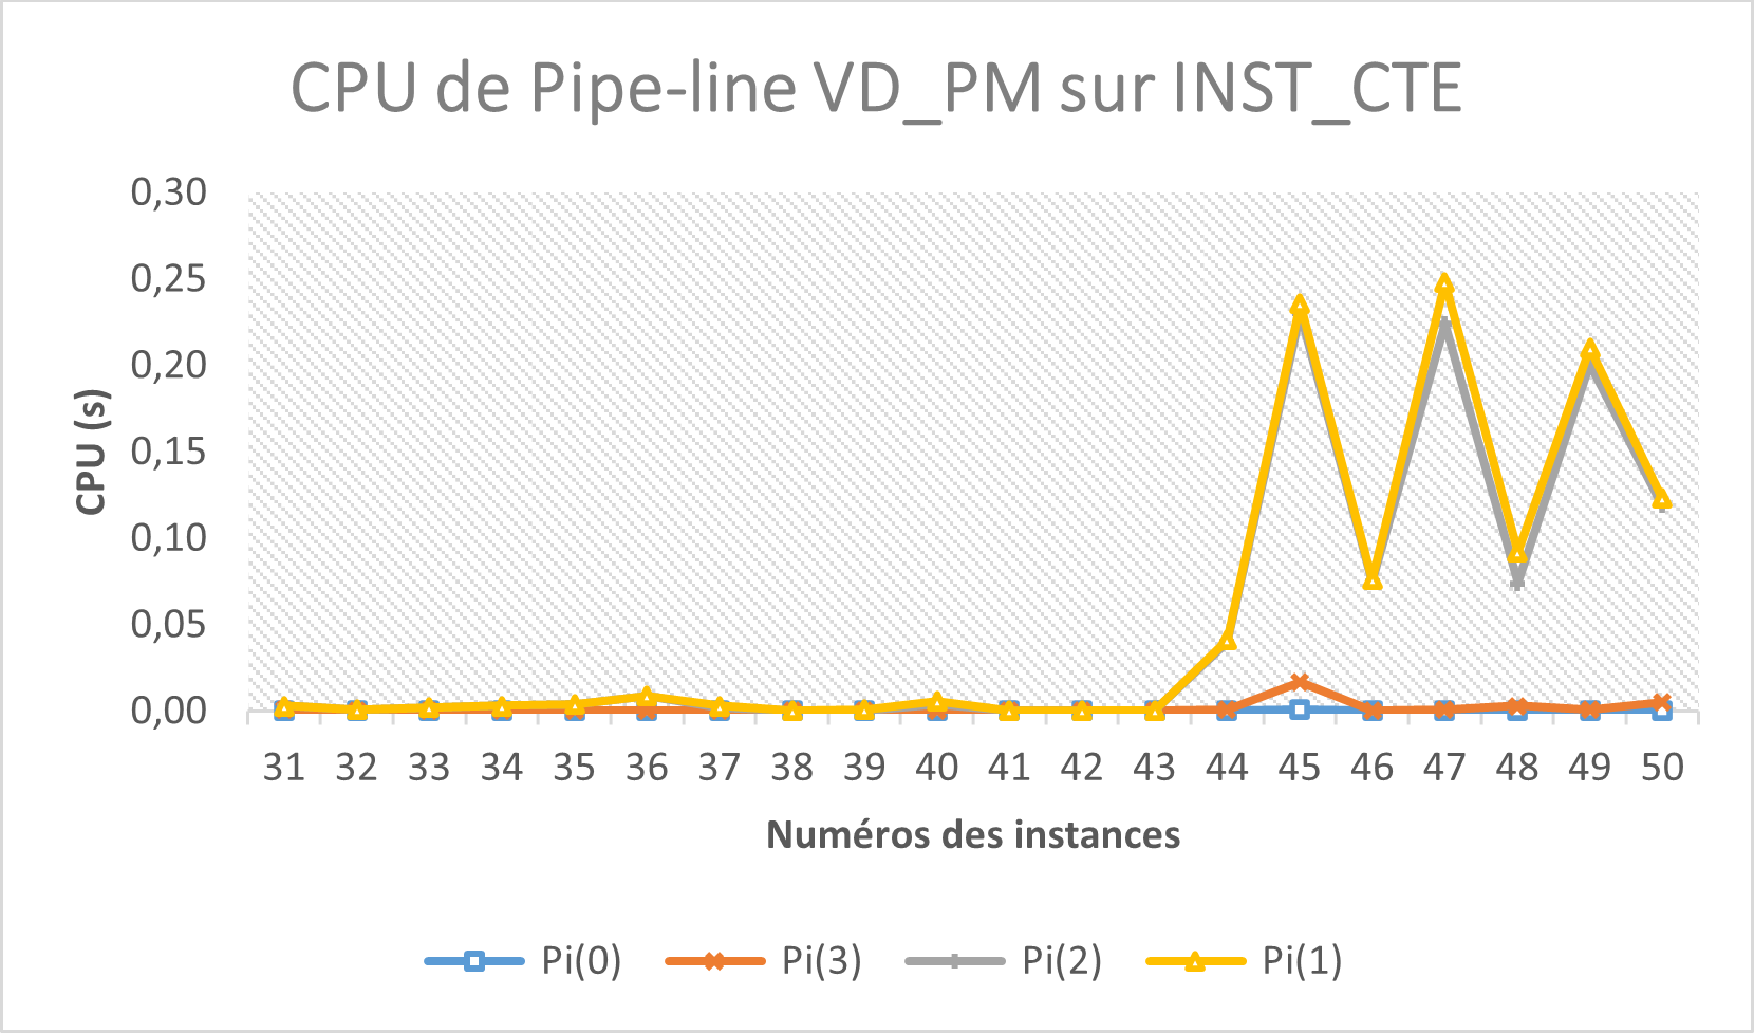
\includegraphics[width=9cm]{images_these/CPU_Pipe_INST_CTE.pdf}&
		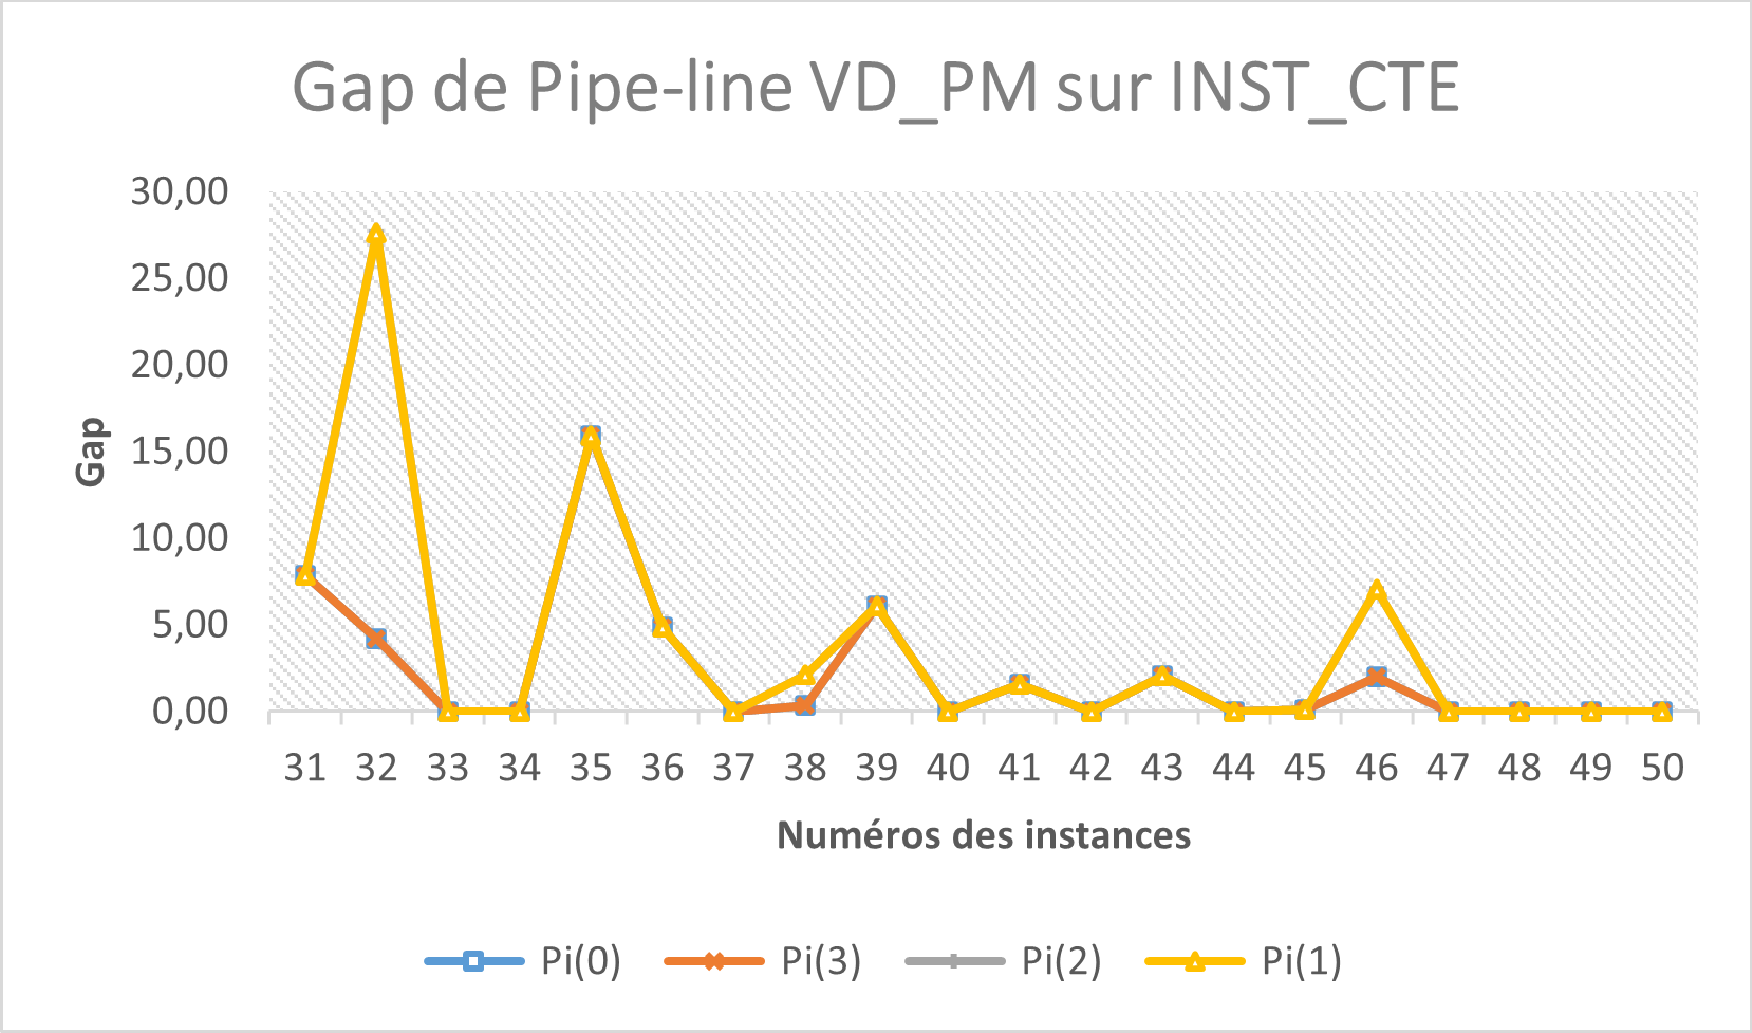
\includegraphics[width=9cm]{images_these/Gap_Pipe_INST_CTE.pdf}
		\\
		(a) & (b)
	\end{tabular}
	\caption[Représentation graphique du CPU et du gap du tableau (\ref{Comparaison_DPS-SMEPC_greed})]{Représentation graphique du tableau (\ref{Comparaison_DPS-SMEPC_greed}). (a) représente le temps CPU et (b) représente le gap de chaque instance de INST\_CTE.}\label{gap_cpu_pipe_INST_}
\end{figure}


\textbf{Comparaison du nombre d'états générés des instances du paquet INST\_CTE :}

Similairement à la section précédente, le tableau (\ref{Comparaison_nombre_state}) présente la comparaison du nombre d'états générés par les algorithmes Pipe-line VD\_PM et DPS\_SMEPC pour les instances du paquet INST\_CTE. Le nombre maximal d'états est appelé $Re$, $Pr$ et $\# Etats$, respectivement pour les algorithmes DPS\_VD, DPS\_PM et DPS\_SMEPC. Le nombre d'états générés par l'algorithme DPS\_VD est inférieur au nombre d'états générés par l'algorithme DPS\_PM ce qui montre que le problème de production est le plus difficile. Le nombre d'états générés par l'algorithme \textbf{DPS\_SMEPC} est supérieur au nombre d'états générés par l'algorithme Pipe-Line VD\_PM.
Globalement le nombre d'états moyen de Pi(0), Pi(3), Pi(2), Pi(1) est respectivement 65,85 ; 407,9 ; 2334 ; 2467,5 
et le nombre d'états moyen de DPS\_SMEPC est respectivement 118,2 ; 13746,85 ; 191125,9 ; 216886,55. 
%On remarque que lorsqu'on ajoute des mécanismes de filtrage l'algorithme est de plus en plus rapide car les mécanismes de filtrage diminue le nombre d'états. En comparant le nombre d'états des algorithmes, on constante que le mécanisme de filtrage exact le plus efficace est le filtrage par estimation optimiste.
%%%%%%%%%%%%%%%%%%%%%%%%%%%%%%%%%%%%%%%%%%%%%%%%%%%%%%%%%%%%%%%%%%%%%%%%%%%%%%%%%%%%%%%%%
\begin{table}[H]
	\centering
	\small
	\begin{tabular}{|r|rrr|rrr|rrr|rrr|}
		\toprule
		\hline
		\rowcolor{cyan}	&\multicolumn{3}{c|}{\textbf{Pi(0)}} & \multicolumn{3}{c|}{\textbf{Pi(3)}}&\multicolumn{3}{c|}{\textbf{Pi(2)}}&\multicolumn{3}{c|}{\textbf{Pi(1)}} \\ \hline
		\midrule
		
		\hline
		\rowcolor{cyan}	&\multicolumn{3}{c|}{ \tiny{Tous les filtrages exacts et heuristiques}} & \multicolumn{3}{c|}{\tiny{Tous les filtrages exacts}}&\multicolumn{3}{c|}{\tiny{Filtrages logiques et optimistes}}&\multicolumn{3}{c|}{\tiny{Sans filtrage}}
		\\ \hline
		\midrule
		
		\rowcolor{cyan}	\textbf{num} & \textbf{Re} & \textbf{Pr} & \textbf{\#Etats} & \textbf{Re} & \textbf{Pr} & \textbf{\#Etats} & \textbf{Re} & \textbf{Pr} & \textbf{\#Etats} &\textbf{Re} & \textbf{Pr} & \textbf{\#Etats} \\ \hline
		\midrule
		31	&	3	&	30	&	131	&	3	&	216	&	3077	&	3	&	689	&	10083	&	3	&	717	&	11422	\\ \hline
		32	&	5	&	9	&	80	&	5	&	9	&	1074	&	5	&	414	&	6042	&	5	&	489	&	6834	\\ \hline
		33	&	3	&	29	&	56	&	3	&	51	&	1670	&	3	&	578	&	11016	&	3	&	580	&	11504	\\ \hline
		34	&	4	&	36	&	120	&	4	&	255	&	5631	&	4	&	701	&	9757	&	4	&	701	&	11491	\\ \hline
		35	&	5	&	69	&	164	&	5	&	238	&	6728	&	5	&	908	&	20679	&	5	&	1030	&	23413	\\ \hline
		36	&	3	&	30	&	48	&	3	&	55	&	531	&	3	&	1429	&	67657	&	3	&	1429	&	68316	\\ \hline
		37	&	4	&	24	&	46	&	4	&	63	&	602	&	4	&	726	&	64720	&	4	&	890	&	66144	\\ \hline
		38	&	4	&	17	&	190	&	4	&	46	&	5513	&	4	&	187	&	11052	&	4	&	312	&	15478	\\ \hline
		39	&	6	&	15	&	110	&	6	&	54	&	8724	&	6	&	393	&	14777	&	6	&	520	&	18045	\\ \hline
		40	&	7	&	13	&	149	&	7	&	64	&	24125	&	7	&	993	&	314059	&	7	&	1393	&	327525	\\ \hline
		41	&	6	&	40	&	301	&	6	&	120	&	35121	&	6	&	198	&	62471	&	6	&	285	&	82386	\\ \hline
		42	&	7	&	44	&	227	&	7	&	155	&	16635	&	7	&	160	&	27568	&	7	&	239	&	40821	\\ \hline
		43	&	7	&	26	&	169	&	7	&	68	&	31508	&	7	&	68	&	31508	&	7	&	68	&	61652	\\ \hline
		44	&	5	&	117	&	75	&	5	&	650	&	4957	&	5	&	3296	&	117870	&	5	&	3296	&	131961	\\ \hline
		45	&	10	&	250	&	73	&	10	&	2329	&	8930	&	10	&	7338	&	221946	&	10	&	7338	&	240786	\\ \hline
		46	&	6	&	37	&	98	&	6	&	118	&	11841	&	6	&	4603	&	388485	&	6	&	4603	&	424646	\\ \hline
		47	&	10	&	93	&	72	&	10	&	578	&	14009	&	10	&	7204	&	841912	&	10	&	7717	&	890054	\\ \hline
		48	&	15	&	80	&	117	&	15	&	1066	&	64992	&	15	&	4045	&	662529	&	15	&	4941	&	893074	\\ \hline
		49	&	10	&	91	&	44	&	10	&	461	&	5497	&	10	&	7377	&	474977	&	10	&	7429	&	501320	\\ \hline
		50	&	10	&	137	&	94	&	10	&	1432	&	23772	&	10	&	5243	&	463410	&	10	&	5243	&	510859	\\ \hline
		
		\bottomrule
	\end{tabular}%
	\caption{Les instances du paquet INST\_CTE : impact des mécanismes de filtrage.}
	
	\label{Comparaison_nombre_state}%
\end{table}%
%%%%%%%%%%%%%%%%%%%%%%%%%%%%%%%%%%%%%%%%%%%%%%%%%%
\begin{figure}[H]
	\centering
	\begin{tabular}{c c}
		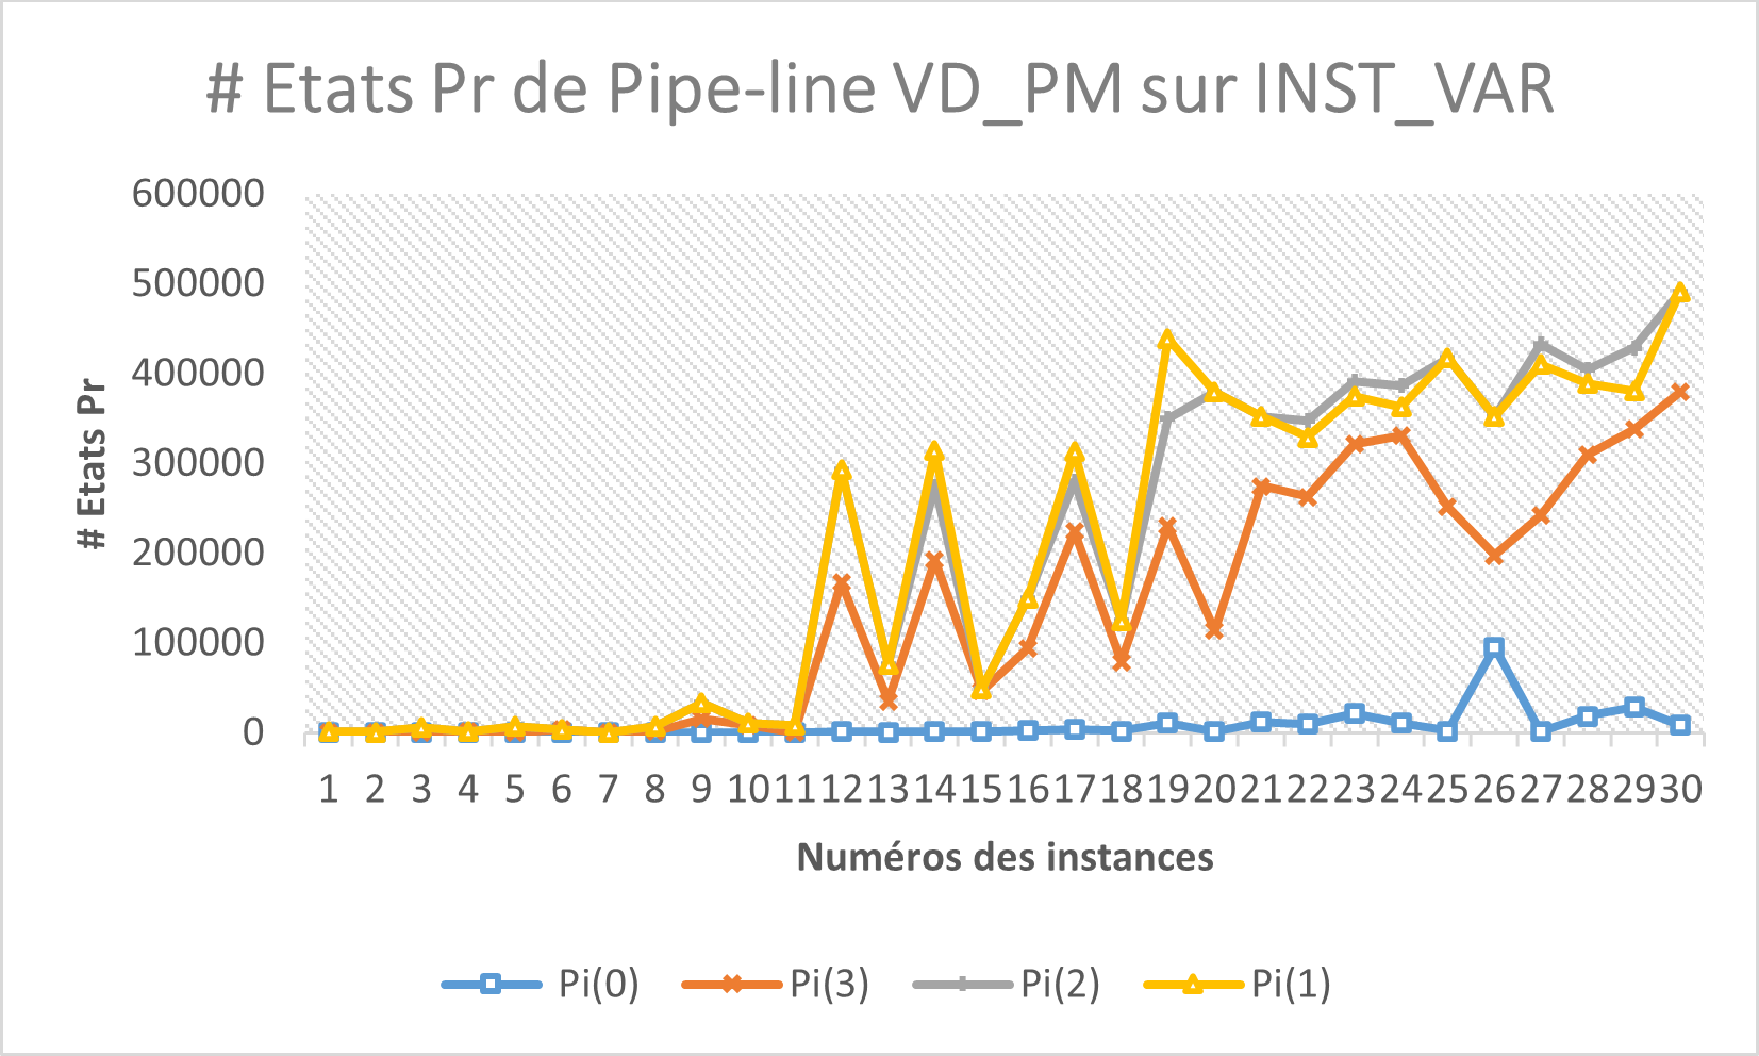
\includegraphics[width=9cm]{images_these/Etat_Pipe_INST_VAR.pdf}&
		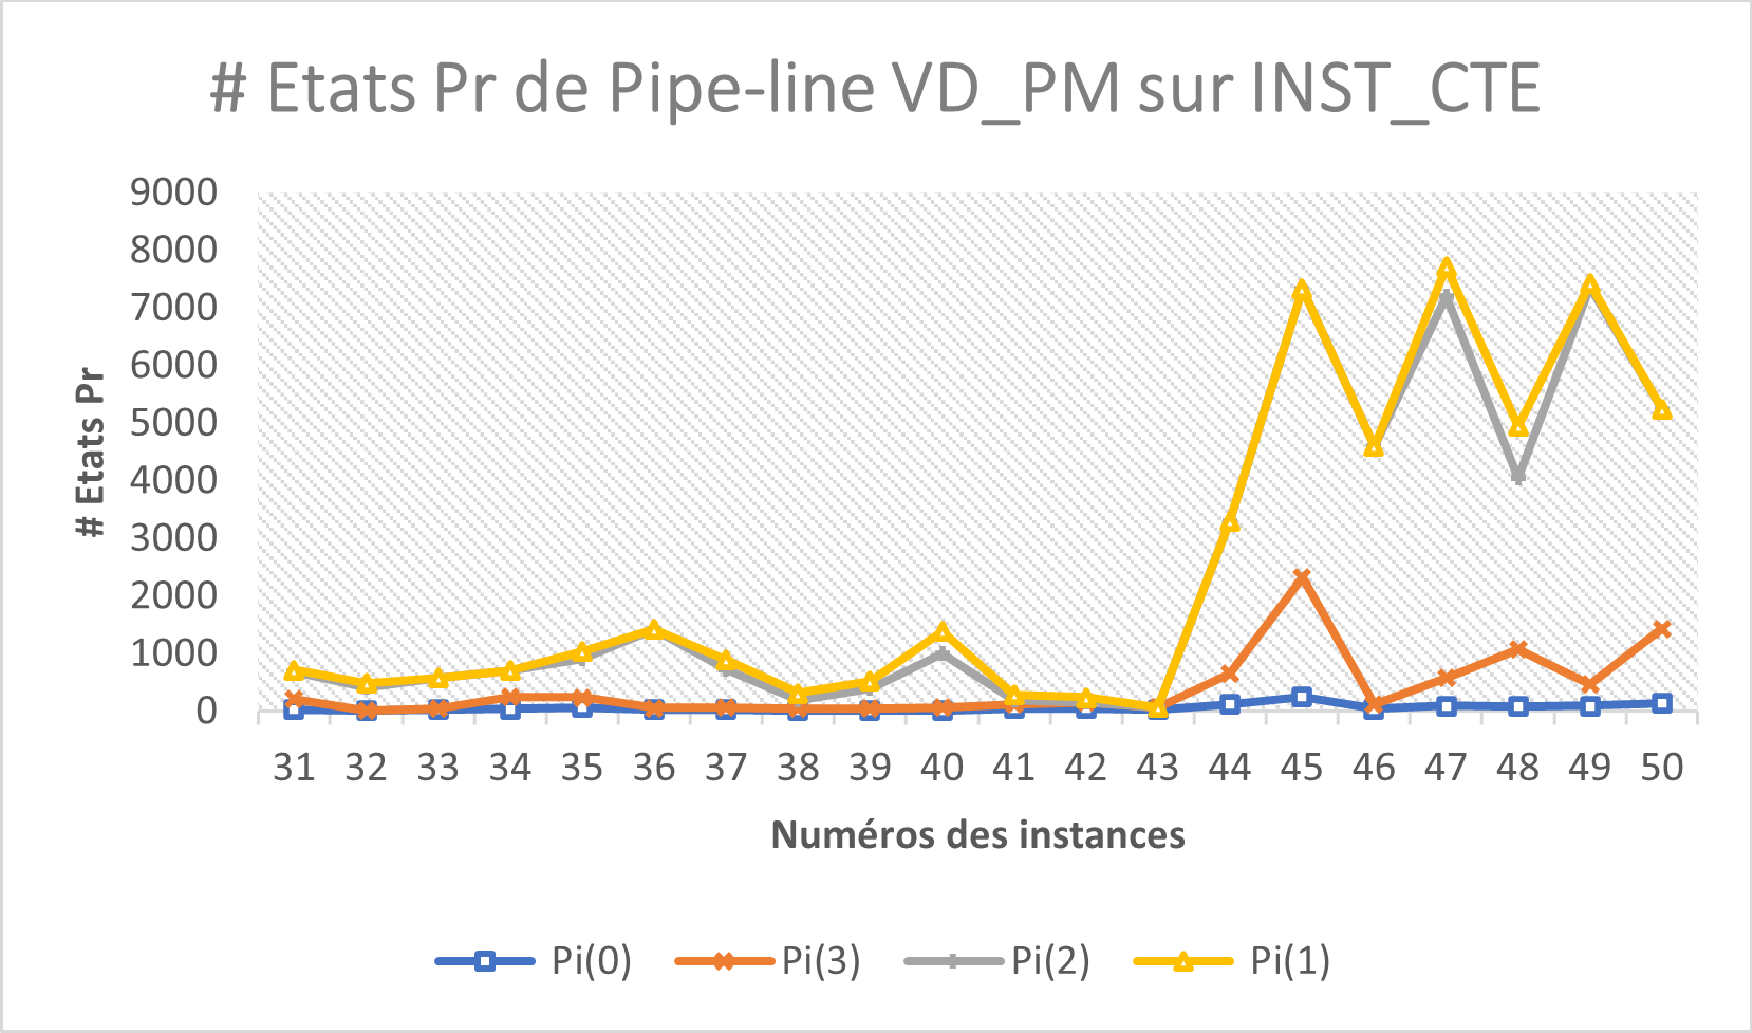
\includegraphics[width=9cm]{images_these/Etat_Pipe_INST_CTE.pdf}
		\\
		(a) & (b)
	\end{tabular}
	\caption[Représentation graphique du CPU et du gap du tableau (\ref{Comparaison_nombre_state2})]{Représentation graphique des tableaux (\ref{Comparaison_nombre_state2}) et (\ref{Comparaison_nombre_state}). (a) représente le nombre d'états de \textbf{Pipe-line VD\_PM} sur INST\_VAR et (b) représente le nombre d'états de \textbf{Pipe-line VD\_PM} sur INST\_CTE.}\label{gap_cpu_pipe_Etat_INST_VAR}
\end{figure}
\subsection{Utilisation de l'algorithme \textbf{Pipe-line VD\_PM} comme borne supérieure du DPS\_SMEPC}

Pour améliorer la procédure général \textbf{DPS\_SMEPC}, on va utiliser la valeur de l'algorithme \textbf{Pipe-line VD\_PM} comme borne supérieure. Dans cette section, on présente les nouveaux résultats du \textbf{DPS\_SMEPC} qu'on a obtenu avec cette nouvelle borne supérieure. Notre objectif ici est de savoir si l'utilisation de la valeur de l'algorithme \textbf{Pipe-line VD\_PM} comme borne supérieure améliore l'algorithme \textbf{DPS\_SMEPC}.
%On cherche à obtenir une évaluation du \textbf{DPS\_SMEPC} lorsqu'on utilise la valeur de l'algorithme \textbf{Pipe-line VD\_PM} comme borne supérieure.
 On cherche à savoir s'il y amélioration du gap par rapport à l'optimalité et s'il y a diminution du nombre d'états générés.
Pour cela, on exécute plusieurs fois l'algorithme \textbf{DPS\_SMEPC} en activant à chaque fois les filtrages qui nous intéressent. La modification de la borne supérieure a un impact uniquement sur $St(0)$ et $St(3)$. On ne calcule pas le gap de $St(3)$ car on obtient la valeur optimale donc le gap vaut zéro. Les tableaux (\ref{BSUPPipe}) et (\ref{BSUPPipe2}) présentent les résultats de l'utilisation de l'algorithme \textbf{Pipe-line VD\_PM} comme borne supérieure du DPS\_SMEPC. En analysant les résultats des instances, on remarque que le filtrage heuristique est efficace car en ajoutant ce filtrage la méthode devient très rapide et de plus les gaps sont inférieurs à 5\%, ces filtrages ne dégradent que légèrement la solution.

Les tableaux (\ref{BSUP_avant_apres_B}) et (\ref{BSUP_avant_apres_A}) comparent les deux bornes supérieures utilisées pour le filtrage respectivement pour le paquet d'instances INST\_CTE et le paquet d'instances INST\_VAR. \og  Search BSUP\fg{} est la borne supérieure calculée par l'algorithme (\ref{Search_BSUP}) présenté au chapitre précédent à la section \ref{Borne_sup}. Et \og Pi(3)\fg{} est la nouvelle borne supérieure obtenue à l'aide de l'algorithme \textbf{Pipe-line VD\_PM}. Globalement, pour les instances pour lesquelles les deux algorithmes donnent des solutions, on remarque que la colonne \og Pi(3)\fg{} donne une meilleure borne supérieure que la colonne \og  Search BSUP\fg{}. Particulièrement, pour onze instances du paquet d'instances INST\_VAR, \og Pi(3)\fg{} ne trouve pas de solutions en moins d'une heure. %On remarque qu'il y a une amélioration de la borne supérieure.

\begin{table}[H]
	\centering
	\small
	\begin{tabular}{|r|rr|rr|}
		\toprule
		\hline
		\rowcolor{cyan}	& \multicolumn{2}{c|}{\textbf{ Search BSUP}}&\multicolumn{2}{c|}{\textbf{Pi(3)}} \\ \hline
		\midrule
		\rowcolor{cyan}	\textbf{num} & \textbf{Obj}& \textbf{Gap}  & \textbf{Obj}& \textbf{Gap}   \\ \hline
		\midrule
		
		1	&	131	&	0,00	&	131	&	0,00	\\ \hline
		2	&	155	&	2,65	&	151	&	0,00	\\ \hline
		3	&	144	&	0,00	&	144	&	0,00	\\ \hline
		4	&	155	&	10,71	&	149	&	6,43	\\ \hline
		5	&	161	&	0,00	&	161	&	0,00	\\ \hline
		6	&	199	&	11,80	&	179	&	0,56	\\ \hline
		7	&	222	&	0,00	&	222	&	0,00	\\ \hline
		8	&	200	&	4,17	&	195	&	1,56	\\ \hline
		9	&	680	&	5,59	&	644	&	0,00	\\ \hline
		10	&	1178	&	3,42	&	1142	&	0,26	\\ \hline
		11	&	140	&	4,48	&	140	&	4,48	\\ \hline
		12	&	970	&	6,36	&	916	&	0,44	\\ \hline
		13	&	970	&	1,46	&	960	&	0,42	\\ \hline
		14	&	1513	&	10,28	&	1387	&	1,09	\\ \hline
		15	&	1371	&	1,86	&	1348	&	0,15	\\ \hline
		16	&	1361	&	5,42	&	1298	&	0,54	\\ \hline
		17	&	1318	&	2,57	&	-	&	-	\\ \hline
		18	&	2490	&	4,93	&	2390	&	0,72	\\ \hline
		19	&	2449	&	10,66	&	-	&	-	\\ \hline
		20	&	2733	&	2,78	&	2679	&	0,75	\\ \hline
		21	&	1529	&	8,44	&	-	&	-	\\ \hline
		22	&	1465	&	9,17	&	-	&	-	\\ \hline
		23	&	2837	&	9,54	&	-	&	-	\\ \hline
		24	&	3058	&	9,02	&	-	&	-	\\ \hline
		25	&	2147	&	4,58	&	-	&	-	\\ \hline
		26	&	2459	&	4,37	&	-	&	-	\\ \hline
		27	&	2543	&	3,04	&	2475	&	0,28	\\ \hline
		28	&	3213	&	5,21	&	-	&	-	\\ \hline
		29	&	4740	&	6,83	&	-	&	-	\\ \hline
		30	&	3621	&	2,81	&	-	&	-	\\ \hline
		
		
		\bottomrule
	\end{tabular}%
	\caption{Les instances du paquet INST\_VAR : Comparaison des deux bornes supérieures utilisées pour le filtrage du DPS\_SMEPC.}
	
	\label{BSUP_avant_apres_B}%
\end{table}%

\begin{table}[H]
	\centering
	\small
	\begin{tabular}{|r|rr|rr|}
		\toprule
		\hline
		\rowcolor{cyan}	& \multicolumn{2}{c|}{\textbf{ Search BSUP}}&\multicolumn{2}{c|}{\textbf{Pi(3)}} \\ \hline
	\midrule
	\rowcolor{cyan}	\textbf{num} & \textbf{Obj}& \textbf{Gap}  & \textbf{Obj}& \textbf{Gap}   \\ \hline
	\midrule
	
	31	&	325	&	34,85	&	260	&	7,88	\\ \hline
	32	&	373	&	4,19	&	373	&	4,19	\\ \hline
	33	&	223	&	0,00	&	223	&	0,00	\\ \hline
	34	&	235	&	16,34	&	202	&	0,00	\\ \hline
	35	&	298	&	15,95	&	298	&	15,95	\\ \hline
	36	&	237	&	4,87	&	237	&	4,87	\\ \hline
	37	&	177	&	0,00	&	177	&	0,00	\\ \hline
	38	&	283	&	0,35	&	283	&	0,35	\\ \hline
	39	&	339	&	8,31	&	332	&	6,07	\\ \hline
	40	&	336	&	0,00	&	336	&	0,00	\\ \hline
	41	&	924	&	2,55	&	915	&	1,55	\\ \hline
	42	&	1440	&	0,00	&	1440	&	0,00	\\ \hline
	43	&	1623	&	5,66	&	1568	&	2,08	\\ \hline
	44	&	919	&	0,00	&	919	&	0,00	\\ \hline
	45	&	947	&	1,94	&	930	&	0,11	\\ \hline
	46	&	868	&	2,00	&	868	&	2,00	\\ \hline
	47	&	942	&	0,00	&	942	&	0,00	\\ \hline
	48	&	1325	&	6,00	&	1250	&	0,00	\\ \hline
	49	&	831	&	0,00	&	831	&	0,00	\\ \hline
	50	&	1084	&	0,37	&	1080	&	0,00	\\ \hline
	
	\bottomrule
\end{tabular}%
\caption{Les instances du paquet INST\_CTE : Comparaison des deux bornes supérieures utilisées pour le filtrage du DPS\_SMEPC.}

\label{BSUP_avant_apres_A}%
\end{table}%


\subsubsection{Utilisation de l'algorithme \textbf{Pipe-line VD\_PM} comme borne supérieure du DPS\_SMEPC : les instances du paquet INST\_VAR}

Le tableau (\ref{BSUPPipe}) présente les résultats des instances du paquet INST\_VAR.  
%On cherche à obtenir une évaluation du \textbf{DPS\_SMEPC} lorsqu'on utilise la valeur de l'algorithme \textbf{Pipe-line VD\_PM} comme borne supérieure. On cherche à savoir s'il y amélioration du gap par rapport à l'optimalité et s'il y a diminution du nombre d'états générés. Pour cela, on exécute plusieurs fois l'algorithme \textbf{DPS\_SMEPC} en activant à chaque fois les filtrages qui nous intéressent. La modification de la borne supérieure a un impact uniquement sur $St(0)$ et $St(3)$. On ne calcule pas le gap de $St(3)$ car on obtient la valeur optimale donc le gap vaut zéro. 
Lorsque la valeur vaut \og - \fg{} cela veut dire que l'algorithme s'est arrêté au bout d'une heure sans trouver de solution.
 % En analysant les résultats des instances du paquet INST\_VAR, on remarque que le filtrage heuristique est efficace car on obtient toujours une solution en moins d'une heure. De plus, en ajoutant le filtrage heuristique la procédure devient très rapide et on obtient des gaps qui sont inférieurs à 5\%, ces filtrages ne dégradent donc que légèrement la solution. 
   La colonne $St(3)$ montre que l'algorithme \textbf{DPS\_SMEPC} ne parvient pas à résoudre 50\% des instances en moins d'une heure. De plus avec le filtrage heuristique on obtient 9 solutions optimales en moins de 0,4 seconde.
Par exemple, pour l'instance 16, on passe de 7,55 minutes de temps d'exécution lorsqu'on exécute sans filtrage heuristique à 0,08 seconde lorsqu'on exécute avec tous les filtrages et on a un gap de 0,08\%. La procédure
 \textbf{DPS\_SMEPC} avec tous les filtrages exactes ($St(3)$) ne parvenait pas à résoudre l'instance 12 en moins d'une heure, or en utilisant la borne supérieure de \textbf{Pipe-line VD\_PM} elle y parvient maintenant en 0,03 seconde. En moyenne sans filtrage heuristique on a généré 629592,9 états et en ajoutant le filtrage heuristique on passe à 1110,767 états  en moyenne. Ce qui nous permet d'affirmer que ce filtrage est efficace.
 Le gap moyen de $St(0)$ est 
 0,23\%. 
 Le nombre d'états moyen de $St(0)$ et $St(3)$ est respectivement 
 1110,767 et 629592,9. 
 Le temps d'exécution moyen en minutes de $St(0)$ et $St(3)$ est respectivement 
 0,16 et 31,25. 
 Dans la section \ref{B_power_filter2} du chapitre précédent, le nombre d'états moyen de $St(0)$ et $St(3)$ était respectivement 2449,133 ; 799762,7333
 et, le temps d'exécution moyen en minutes était respectivement 0,96 ; 36,1048.
 De plus, le gap moyen de $St(0)$ était 0,596\%.
  En comparant le tableau (\ref{BSUPPipe}) à celui de la section \ref{B_power_filter2}, on constate qu'il y a une diminution du gap, du temps d'exécution et du nombre d'états générés par l'algorithme \textbf{DPS\_SMEPC}. Ce qui prouve que l'utilisation de la valeur du Pipe-Line VD\_PM comme borne supérieure a amélioré la procédure DPC\_SMEPC.
  
%%%%%%%%%%%%%%%%%%%%%%%%%%%%%%%%%%%%%%%%%%%%%%%%%%%%%%%%%%%%%%%%%%%%%%%%%%%%%%%%%%%%%%%%%
\begin{table}[H]
	\centering
	\small
	\begin{tabular}{|r|rrrr|rrr|}
		\toprule
		\hline
		\rowcolor{cyan}	&\multicolumn{4}{c|}{\textbf{St(0)}} & \multicolumn{3}{c|}{\textbf{St(3)}}\\ \hline
		\midrule
			\hline
		\rowcolor{cyan}	&\multicolumn{4}{c|}{ \scriptsize{Tous les filtrages exacts et heuristiques}} & \multicolumn{3}{c|}{\scriptsize{Tous les filtrages exacts}}
		\\ \hline
		\midrule
	
		\rowcolor{cyan}	\textbf{num} &\textbf{Obj} & \textbf{Gap} & \textbf{\#Etats} & \textbf{CPU} &\textbf{Obj} & \textbf{\#Etats} & \textbf{CPU}   \\ \hline
		\midrule
		
		1	&	131	&	0,00	&	61	&	0,00	&	131	&	554	&	0,00	\\ \hline
		2	&	151	&	0,00	&	159	&	0,00	&	151	&	1336	&	0,01	\\ \hline
		3	&	144	&	0,00	&	63	&	0,00	&	144	&	2213	&	0,03	\\ \hline
		4	&	140	&	0,00	&	281	&	0,01	&	140	&	1844	&	0,02	\\ \hline
		5	&	161	&	0,00	&	48	&	0,00	&	161	&	406	&	0,01	\\ \hline
		6	&	179	&	0,56	&	78	&	0,00	&	178	&	2472	&	0,04	\\ \hline
		7	&	222	&	0,00	&	126	&	0,00	&	222	&	1732	&	0,01	\\ \hline
		8	&	192	&	0,00	&	72	&	0,00	&	192	&	965	&	0,01	\\ \hline
		9	&	644	&	0,00	&	161	&	0,01	&	644	&	6962	&	0,18	\\ \hline
		10	&	1142	&	0,26	&	102	&	0,01	&	1139	&	49609	&	2,37	\\ \hline
		11	&	140	&	4,48	&	29	&	0,00	&	134	&	536	&	0,01	\\ \hline
		12	&	914	&	0,22	&	176	&	0,03	&	912	&	12756	&	1,67	\\ \hline
		13	&	960	&	0,42	&	58	&	0,00	&	956	&	3391	&	0,15	\\ \hline
		14	&	1372	&	0,00	&	460	&	0,31	&	-	&	754539	&	3600,43	\\ \hline
		15	&	1348	&	0,15	&	88	&	0,02	&	1346	&	88677	&	22,87	\\ \hline
		16	&	1292	&	0,08	&	230	&	0,08	&	1291	&	327838	&	453,14	\\ \hline
		17	&	1288	&	0,23	&	410	&	0,73	&	-	&	900272	&	3615,24	\\ \hline
		18	&	2383	&	0,42	&	257	&	0,20	&	-	&	939836	&	3740,62	\\ \hline
		19	&	2218	&	0,23	&	724	&	2,13	&	-	&	1908524	&	3669,73	\\ \hline
		20	&	2655	&	-0,15	&	498	&	1,00	&	-	&	1180949	&	3631,16	\\ \hline
		21	&	1412	&	0,14	&	2037	&	17,51	&	-	&	1216931	&	3626,03	\\ \hline
		22	&	1350	&	0,60	&	1086	&	3,33	&	-	&	773791	&	3600,59	\\ \hline
		23	&	2596	&	0,23	&	745	&	2,53	&	-	&	1076713	&	3805,69	\\ \hline
		24	&	2807	&	0,07	&	629	&	2,25	&	-	&	1443810	&	3949,79	\\ \hline
		25	&	2060	&	0,34	&	1052	&	8,05	&	-	&	1683461	&	3626,42	\\ \hline
		26	&	2353	&	-0,13	&	18731	&	205,21	&	-	&	817959	&	3655,21	\\ \hline
		27	&	2475	&	0,28	&	488	&	1,39	&	-	&	704556	&	3606,82	\\ \hline
		28	&	3066	&	0,39	&	1997	&	13,72	&	-	&	1357220	&	4288,92	\\ \hline
		29	&	4377	&	-1,35	&	1122	&	4,11	&	-	&	1861070	&	3707,21	\\ \hline
		30	&	3500	&	-0,62	&	1355	&	20,32	&	-	&	1766865	&	3646,29	\\ \hline
		
		\bottomrule
	\end{tabular}%
	\caption{Les instances du paquet INST\_VAR : impact des mécanismes de filtrage du DPS\_SMEPC.}
	\label{BSUPPipe}%
\end{table}%
%%%%%%%%%%%%%%%%%%%%%%%%%%%%%%%%%%%%%%%%%%%%%%%%%%

\subsubsection{Utilisation de l'algorithme \textbf{Pipe-line VD\_PM} comme borne supérieure du DPS\_SMEPC : les instances du paquet INST\_CTE}

Le tableau (\ref{BSUPPipe2}) présente les résultats des instances du paquet INST\_CTE. 
%On cherche à obtenir une évaluation du \textbf{DPS\_SMEPC} lorsqu'on utilise la valeur de l'algorithme \textbf{Pipe-line VD\_PM} comme borne supérieure. On cherche à savoir s'il y amélioration du gap par rapport à l'optimalité et s'il y a diminution du nombre d'états générés. Pour cela, on exécute plusieurs fois l'algorithme \textbf{DPS\_SMEPC} en activant à chaque fois les filtrages qui nous intéressent. La modification de la borne supérieure a un impact uniquement sur $St(0)$ et $St(3)$. On ne calcule pas le gap de $St(3)$ car on obtient la valeur optimale donc le gap vaut zéro.
%En analysant les résultats des instances du paquet INST\_CTE, on remarque que le filtrage heuristique est efficace car en ajoutant ce filtrage la méthode devient très rapide et de plus les gaps sont inférieurs à 5\%, ces filtrages ne dégradent que légèrement la solution.
En ajoutant le filtrage heuristique, on obtient 70\% de solutions optimales. Par exemple, pour l'instance 48, on passe de 15,54 secondes de temps d'exécution lorsqu'on exécute sans filtrage heuristique à 0,01 seconde lorsqu'on exécute avec le filtrage heuristique et on obtient la solution optimale. 
En moyenne sans filtrage heuristique, on a généré 12489,1 états et en ajoutant le filtrage heuristique on passe à 112,75 en moyenne d'états générés. Ce qui nous permet d'affirmer une fois de plus que ce filtrage est efficace.
Le gap moyen de St(0)  est 
0,562\%. 
Le nombre d'états moyen de St(0) et St(3) est respectivement 
112,75 et 12489,1. 
Le temps d'exécution moyen en secondes de St(0) et St(3) est respectivement 
0,0068 et 1,54. 
Dans la section \ref{A_power_filter2} du chapitre précédent, le nombre d'états moyen de St(0), St(3) était respectivement 118,2; 13746,85 
et le temps d'exécution moyen en secondes était respectivement 0,007; 2,448. De plus le gap moyen de $St(0)$ était 1,108\%.
En comparant le tableau (\ref{BSUPPipe2}) à celui de la section \ref{A_power_filter2}, on constate qu'il y a une diminution du gap, du temps d'exécution et du nombre d'états générés par l'algorithme \textbf{DPS\_SMEPC}. Comme à la section précédente, ceci prouve que l'utilisation de la valeur du Pipe-Line VD\_PM comme borne supérieure a amélioré la procédure DPS\_SMEPC.


%%%%%%%%%%%%%%%%%%%%%%%%%%%%%%%%%%%%%%%%%%%%%%%%%%%%%%%%%%%%%%%%%%%%%%%%%%%%%%%%%%%%%%%%%
\begin{table}[H]
	\centering
	\small
	\begin{tabular}{|r|rrrr|rrr|}
		\toprule
		\hline
		\rowcolor{cyan}	&\multicolumn{4}{c|}{\textbf{St(0)}} & \multicolumn{3}{c|}{\textbf{St(3)}}\\ \hline
		\midrule
		
		\hline
		\rowcolor{cyan}	&\multicolumn{4}{c|}{ \scriptsize{Tous les filtrages exacts et heuristiques}} & \multicolumn{3}{c|}{\scriptsize{Tous les filtrages exacts}}
		\\ \hline
		
		\midrule
		\rowcolor{cyan}	\textbf{num} &\textbf{Obj} & \textbf{Gap} & \textbf{\#Etats} & \textbf{CPU} &\textbf{Obj} & \textbf{\#Etats} & \textbf{CPU}   \\ \hline
		\midrule
		31	&	241	&	0,00	&	115	&	0,00	&	241	&	2341	&	0,02	\\ \hline
		32	&	373	&	4,19	&	80	&	0,00	&	358	&	1074	&	0,01	\\ \hline
		33	&	223	&	0,00	&	56	&	0,00	&	223	&	1670	&	0,01	\\ \hline
		34	&	202	&	0,00	&	96	&	0,00	&	202	&	3058	&	0,04	\\ \hline
		35	&	257	&	0,00	&	164	&	0,01	&	257	&	6728	&	0,11	\\ \hline
		36	&	226	&	0,00	&	48	&	0,00	&	226	&	531	&	0,01	\\ \hline
		37	&	177	&	0,00	&	46	&	0,00	&	177	&	602	&	0,01	\\ \hline
		38	&	282	&	0,00	&	190	&	0,01	&	282	&	5513	&	0,06	\\ \hline
		39	&	323	&	3,19	&	100	&	0,00	&	313	&	7397	&	0,06	\\ \hline
		40	&	336	&	0,00	&	149	&	0,01	&	336	&	24125	&	0,68	\\ \hline
		41	&	915	&	1,55	&	276	&	0,02	&	901	&	34026	&	3,56	\\ \hline
		42	&	1440	&	0,00	&	227	&	0,02	&	1440	&	16635	&	1,28	\\ \hline
		43	&	1568	&	2,08	&	169	&	0,01	&	1536	&	31508	&	2,75	\\ \hline
		44	&	919	&	0,00	&	75	&	0,00	&	919	&	4957	&	0,19	\\ \hline
		45	&	930	&	0,11	&	63	&	0,00	&	929	&	7534	&	0,49	\\ \hline
		46	&	852	&	0,12	&	98	&	0,02	&	851	&	11841	&	1,11	\\ \hline
		47	&	942	&	0,00	&	72	&	0,01	&	942	&	14009	&	1,48	\\ \hline
		48	&	1250	&	0,00	&	93	&	0,01	&	1250	&	48374	&	15,54	\\ \hline
		49	&	831	&	0,00	&	44	&	0,01	&	831	&	5497	&	0,51	\\ \hline
		50	&	1080	&	0,00	&	94	&	0,01	&	1080	&	22362	&	2,89	\\ \hline
		
		\bottomrule
	\end{tabular}%
	\caption{Les instances du paquet INST\_CTE : impact des mécanismes de filtrage du DPS\_SMEPC.}
	\label{BSUPPipe2}%
\end{table}%
%%%%%%%%%%%%%%%%%%%%%%%%%%%%%%%%%%%%%%%%%%%%%%%%%%


\section{Conclusion}
Nous avons présenté un schéma de programmation dynamique collaboratif afin de résoudre le problème SMEPC qui nécessite des mécanismes de synchronisation.
Comme nous l'avons dit au début de ce chapitre, notre principal objectif ici est de mettre en œuvre la synchronisation tout en émulant les interactions qui sont susceptibles d'avoir lieu entre les acteurs décentralisés. Le mécanisme de pipeline à sens unique qu'on a implémenté est clairement l'un des plus simples. Mais on pourrait penser à concevoir des schémas d'interaction plus sophistiqués, et même si nous nous limitons à ce schéma spécifique, certains points peuvent être discutés :
%\begin{itemize}[label=$\square$]
	sur la simple structure de l'algorithme \textbf{Pipe-line VD\_PM}
	,le lien entre \textbf{VD} et \textbf{PM} défini par $\beta$ se comporte ici comme un lien monodirectionnel : On attribue une valeur à $\beta$ , et on lance successivement \textbf{DPS\_VD} et \textbf{DPS\_PM}. Mais on peut se demander comment récupérer des informations de cette séquence \textbf{DPS\_VD $\rightarrow$ DPS\_PM} et s'adapter en conséquence. Par exemple, on peut essayer ceci : après chaque exécution de la séquence \textbf{DPS\_VD $\rightarrow$ DPS\_PM}, attribuer à $\beta$ une nouvelle valeur $\beta^*$ telle que la quantité $\beta^* \times (\sum_j L_j \times x_j)$ devienne égale au coût énergétique $\sum_{i = 0, \dots, N -1} (Cost^F\times y_i + Cost^V_i\times z_i)$ et recommencer le processus. Nous n'avons pas essayé cette option, principalement parce qu'elle prend beaucoup de temps. De la même manière, on pourrait faire en sorte que le coefficient $\alpha$ qui pondère les temps d'attente que le conducteur du véhicule doit accepter fasse partie du processus de négociation.
	
	%\item À propos du choix de $\beta$: il doit refléter le coût de production de l'énergie qui doit être produite. Mais, comme nous ne connaissons pas a priori la répartition temporelle des opérations de recharge, nous divisons l'intervalle de temps en 3 macro-périodes et faisons comme si cette répartition devait être uniforme entre ces macro-périodes. Nous avons donc fixé :
	%\begin{itemize}
	%	\item $H =$ Energie que le véhicule doit charger en fonction du modèle \textbf{VD} avec $\beta= 1$ et $\alpha= 0$ ;
	%	\item $Rough\_Cost = CostMin(0, H/3 , 0) + CostMin(\lfloor N/3\rfloor, H/3 , 0) + CostMin(\lfloor2\times N/3\rfloor, H/3 , 0) $;
	%	\item $\beta = Rough\_Cost/H$.
		
	%\end{itemize}
	%\item À propos de la spécification du modèle \textbf{VD} : Nous pouvons remarquer qu'il serait possible de traiter la \textbf{VD} de la même manière que nous l'avons fait, tout en remplaçant le terme $\beta \times (\sum_j L_j\times x_j)$ de la fonction objectif par un terme $  (\sum_j \beta_j \times L_j\times x_j)$, ce qui nous donnerait plus de flexibilité. Néanmoins, anticiper le prix de la quantité d'hydrogène chargée par le véhicule à l'arrêt resterait une difficulté.
	
	
%\end{itemize} 
\section{Annexes}
\subsection{Démonstration du théorème \ref{vd_ndhard}}
\label{vd_ndhard_section}
Cette section présente la démonstration du théorème \ref{vd_ndhard} : Si nous imposons que tout $L_j$ est soit nul ou égal à une constante $R$, alors \textbf{VD} devient NP-Hard.

%\textbf{Démonstration} : Pour tout j, fixons : $A_j = d_j + d^*_{j+1} - t_j $ et $ B_j = H - (\varepsilon_j + \varepsilon^*_{j+1} - e_j)$. Fixons également $C=\sum_j e_j$. Enfin supposons $C^{Veh}=+\infty$, $\beta=0$ et $TMax=+\infty$. Nous voyons que $x$ devrait être tel que :
%\begin{itemize}
%	\item $\sum_j x_j\times B_j \geq C$ ;
%	\item $\sum_j x_j \times A_j$ est le plus petit possible.
%\end{itemize}

%Selon ces hypothèses, \textbf{VD} coïncide avec le problème du sac à dos. Inversement, toute instance du problème du sac à dos peut être transformée en une instance de \textbf{VD}.

% Dans un premier temps, pour montrer que ce problème est NP, on a montrer qu'on peut le formuler avec un PLNE sans faire exploser la taille. 
%Dans un second temps, 
Dans cette partie nous allons démontrer que le problème VD avec $L_j$ fixe est un problème NP-Hard.
Nous allons montrer que le problème VD avec $L_j$ fixe se réduit en temps polynomial au problème du sac à dos inversé.
La formulation du problème du sac à dos ($K$) est la suivante :
\og Étant  donnés  $n$  objets  possédant chacun  un  poids $p_i$ et une  valeur $v_i$, $i=\{1, \dots n\}$. Étant  donné un sac de poids  maximum $b$,  quels  objets faut-il  mettre  dans  le  sac  de  manière  à  maximiser  la  valeur  totale  sans  dépasser  le  poids maximal du sac ? \fg{}  La modélisation de ($K$) sous forme de programme linéaire en nombres entiers est la suivante :

Soit un sac à dos de poids maximal $b$ et $n$ objets. Pour chaque objet $i$, nous avons un poids $p_i \geq 0$ et une valeur $v_i \geq 0$,

\begin{itemize}
	
	\item La variable de décisions est $y_i$ avec $i \in \{1, 2, \dots ,n\}$
	$$
	y_i = \left\{
	\begin{array}{ll}
	1 & \mbox{si l'objet i est mis dans le sac} \\
	0 & \mbox{sinon.}
	\end{array}
	\right.
	$$
	\item La contrainte est $\sum_{i=1}^{n} p_i \times y_i \leq b$ car le sac à dos à un poids maximum $b$ qu'il ne faut pas dépasser ;
	\item La fonction objectif à maximiser est $\sum_{i=1}^{n} v_i \times y_i$ car l'objectif est de maximiser la valeur totale des objets introduit dans le sac à dos.
	
	
	
\end{itemize}
Nous devons faire apparaitre le problème du sac à dos inversé comme un cas particulier du problème VD avec $L_j$ fixe. Pour cela, à une instance $(n,P_i,v_i,b)$ du problème du sac à dos inversé, on doit associer  à l'aide de formules une instance $(M, t_j, d_j, d_j^*, e_j, \varepsilon_{j}, \varepsilon_{j}^*, R, E_0, C^{Veh})$ du problème VD avec $L_j$ fixe dont la signification est : $M$ est le nombre de stations, les distances entre les stations sont ($t_j, d_j, d_j^*$), les quantités d'énergies dépensées lors des trajets sont ($ e_j, \varepsilon_{j}, \varepsilon_{j}^*$), la quantité d'hydrogène chargée est ($R$), l'énergie initiale du véhicule est ($E_0$) et le capacité maximal du réservoir d'hydrogène est ($C^{Veh}$). 

Une fois ces formules obtenues :
\begin{enumerate}
	\item on veut montrer que $(M, t_j, d_j, d_j^*, e_j, \varepsilon_{j}, \varepsilon_{j}^*, R, E_0, C^{Veh})$ nous donne bien une instance du problème VD avec $L_j$ fixe, et donc qu'on a $t_j$, $d_j$, $d_j^*$ et $ , e_j$, $\varepsilon_{j}$, $\varepsilon_{j}^*$ qui sont des distances qui respectent l'inégalité du triangle. De plus, il faut que $t_j\geq 0$, $d_j\geq 0$, $d_j^* \geq 0$ et $e_j\geq 0$, $\varepsilon_{j}\geq 0$, $ \varepsilon_{j}^* \geq 0$.
	\item on veut montrer qu'une solution optimale du problème du sac inversé à dos s'interprète comme une solution optimale du problème VD avec $L_j$ fixe.
\end{enumerate}
Pour faire apparaitre les stations, on pose $n=M$, $y_i=1-x_i$, $i=1,\dots, n$ avec $x_i \in \{0,1\}$, $(K)$ devient :

$$\left\{
\begin{array}{l}

Maximiser : \sum_{i=1}^{n} v_i \times (1-x_i)=\sum_{i=1}^{n}v_i -\sum_{i=1}^{n}v_i \times x_i\\
st : -\sum_{i=1}^{n} p_i \times x_i \leq -\sum_{i=1}^{n}p_i+b
\end{array}
\right.$$

Car $(1-x_i)  \in \{0,1\} \Rightarrow x_i  \in \{0,1\}$

c'est-à-dire,

$$
\left\{
\begin{array}{l}

Minimiser :- \sum_{i=1}^{n} v_i+\sum_{i=1}^{n} v_i \times x_i  \\
st : \sum_{i=1}^{n} p_i \times x_i \geq (\sum_{i=1}^{n}p_i)-b
\end{array}
\right.$$
Car Zmax(X)=-Zmin(-X)

En ce qui concerne la capacité du réservoir d'hydrogène nous allons considérer qu'on a un véhicule dont la capacité du réservoir est très grande. Dans ce cadre là, l'objectif est de minimiser $\sum_{i=1}^{n} (d_{i}+d_{i+1}^*-t_i) \times x_i$ sous les contraintes (\ref{eqop0}), (\ref{eqopj}) et  (\ref{eqop}).

\begin{equation}
\label{eqop0}
\boxed{
\begin{array}{l}
E_0 - \varepsilon_{1}^*-(\varepsilon_{1} \times x_1)   \geq 0
\end{array}
}
\end{equation}

\begin{equation}
\label{eqopj}
\boxed{
\begin{array}{l}
\sum_{j=1}^{i}[(R + e_j- (\varepsilon_{j}+\varepsilon_{j+1}^*)) \times x_j] -(\varepsilon_{i+1} \times x_{i+1})   \geq  \varepsilon_{1}^*+ \sum_{j=1}^{i}e_j -E_0
\end{array}
}
\end{equation}
avec $i \in 1\dots n -1$

\begin{equation}
\label{eqop}
\boxed{
\begin{array}{l}
\sum_{i=1}^{n}[(R + e_{i}-(\varepsilon_{i}+\varepsilon_{i+1}^* )) \times x_i]   \geq  \varepsilon_{1}^*+ \sum_{i=1}^{n}e_i+\varepsilon_{n} -E_0
\end{array}
}
\end{equation}




% En posant,

% $\left\{
% \begin{array}{l}
%p_i= R +e_i-(\varepsilon_{i}+\varepsilon_{i+1}^*)\\
%%b'=-E_0+ \varepsilon_{1}^*+ \sum_{j=1}^{n}(e_i)+\varepsilon_{n}\\
%v_i=d_{i}+d_{i+1}^*-t_i
% \end{array}
% \right.$
On pose $v_{0}=p_{0}=v_{n+1}=p_{n+1}=0$. Pour obtenir les distances entre les stations et les quantités d'énergies dépensées lors des trajets, posons :
\begin{itemize}

\item  $t_i=\frac{v_{i+1}+v_{i-1}}{2}, d_{i}^*=d_{i}=\frac{v_{i}+v_{i-1}}{2} $, pour  $i=1,\dots, n$

\item $e_i=R- \frac{p_{i+1}+p_{i-1}}{2}$, $\varepsilon_{i}^*=\varepsilon_{i}=R-\frac{p_{i}+p_{i-1}}{2}  $, pour  $i =1, \dots,  n$,

avec la quantité d'hydrogène chargée $R$ qui vaut $R = \textrm{max}(p_i) $.% et $p_0=0$

\item La quantité d'hydrogène initialement dans le véhicule est :

$E_0 = \varepsilon_{1}^*+ \sum_{j=1}^{n}e_j+ max_{1 \leq i \leq n}(\varepsilon_{i})$

\item $\varepsilon_{n} =(\sum_{i=1}^{n}p_i)-b+ max_{1 \leq i \leq n}(\varepsilon_{i})$

\end{itemize}


Les $p_i$ et $v_i$ peuvent être quelconques mais les $t_j, d_j, d_j^*$ et $e_j, \varepsilon_{j}, \varepsilon_{j}^*$  doivent respecter l'inégalité triangulaire parce qu'elles doivent correspondre à des distances, nous vérifions alors que :


\begin{enumerate}
\item $
d_{i}+d_{i+1}^*-t_i=  \frac{v_{i}+v_{i-1}}{2}   + 
\frac{v_{i+1}+v_{i}}{2}   - 
\frac{v_{i+1}+v_{i-1}}{2} =v_i$, pour $i=1, \dots,  n$

donc $t_i \leq d_{i}+d_{i+1}^*$


\item $
d_{i+1}^*+t_i-d_{i}=  \frac{v_{i+1}+v_{i}}{2}   + 
\frac{v_{i+1}+v_{i-1}}{2} -\frac{v_{i}+v_{i-1}}{2}   =v_{i+1}$, pour $i=1, \dots,  n$

donc $d_{i} \leq t_i+d_{i+1}^*$


\item $
t_i+d_{i}-d_{i+1}^*=  \frac{v_{i+1}+v_{i-1}}{2} +
\frac{v_{i}+v_{i-1}}{2}  -\frac{v_{i+1}+v_{i}}{2}   +  =v_{i-1}$, pour $i=1, \dots,  n$

donc $d_{i+1} \leq t_i+d_{i}^*$

\item $
\varepsilon_{i}+\varepsilon_{i+1}^*-e_i=R- \frac{p_{i}+p_{i-1}}{2} +  R- 
\frac{p_{i+1}+p_{i}}{2}   - R+
\frac{p_{i+1}+p_{i-1}}{2} =R-p_i$, pour $i=1, \dots,  n$

donc $e_i \leq \varepsilon_{i}+\varepsilon_{i+1}^*$ car $R = \textrm{max}(p_i) $


\item $
\varepsilon_{i}+e_i-\varepsilon_{i+1}^*=R- \frac{p_{i}+p_{i-1}}{2} +  R-
\frac{p_{i+1}+p_{i-1}}{2} - R+ 
\frac{p_{i+1}+p_{i}}{2}  =R-p_{i-1}$, pour $i=1, \dots,  n$

donc $\varepsilon_{i+1}^* \leq \varepsilon_{i}+e_i$ car $R = \textrm{max}(p_i) $


\item $
\varepsilon_{i+1}^*+e_i-\varepsilon_{i}=  R- \frac{p_{i+1}+p_{i}}{2}   + R-
\frac{p_{i+1}+p_{i-1}}{2}- R+ \frac{p_{i}+p_{i-1}}{2}  =R-p_{i+1}$, pour $i=1, \dots,  n$

donc $\varepsilon_{i} \leq \varepsilon_{i+1}^*+e_i$ car $R = \textrm{max}(p_i) $



\end{enumerate}

$R+e_i-(\varepsilon_{i}+\varepsilon_{i+1}^*)=2R- \frac{p_{i+1}+p_{i-1}}{2}   - 2R+ \frac{p_{i}+p_{i-1}}{2}  + \frac{p_{i+1}+p_{i}}{2} =p_i$, pour $i=1, \dots,  n$

et le second membre de (\ref{eqop}) devient,



$ \varepsilon_{1}^*+ \sum_{j=1}^{n}e_j -E_0 +\varepsilon_{n} =(\sum_{i=1}^{n}p_i)-b $

et les seconds membres de (\ref{eqopj}) sont tous négatifs ou nuls car 

$E_0 \geq \varepsilon_{1}^*+ \sum_{j=1}^{i}e_j+\varepsilon_{i+1}$.


Il reste à vérifier l'inéquation (\ref{eqop}).  
$ \sum_{j=1}^{i}[(R + e_j- (\varepsilon_{j}+\varepsilon_{j+1}^*)) \times x_j]   \geq  \varepsilon_{1}^*+ \sum_{j=1}^{i}e_j -E_0 $ est aussi vrai avec $i=\{2, \dots, n\}$
On a donc démontré que résoudre le problème VD avec $L_j$ fixe revient donc à résoudre le problème $(K)$.  $\square$
%La fonction $\pi$ est 

%$\begin{array}{ccccc}
% & : & E & \to & F \\
%& & \alpha & \mapsto & \pi(\alpha)=\alpha \\
%\end{array}$
%%%%%%%%%%%%%%%part1

%\begin{Rem}
%Cette démonstration est valable s'il n'existe aucune relation entre  $t_j, d_j, d_j^*$ et $e_j, \varepsilon_{j}, \varepsilon_{j}^*$. Il peut arriver que la longueur d'un parcourt soit proportionnelle à la quantité d'énergie nécessaire pour effectuer ce parcourt. Dans ce cas, il faudra donc vérifier que cette relation est vérifiée.
%\end{Rem}
\subsection{Démonstration du théorème \ref{VD_polynomial}}
\label{VD_polynomial_section}
Cette section présente la démonstration du théorème \ref{VD_polynomial}.
Dans cette section, nous allons prouver que \textbf{VD} est polynomiale. Cependant, nous sommes toujours à la frontière entre P et NP.

\textbf{Le graphe VD\_Graph} : Afin de traiter le problème \textbf{VD}, nous allons faire apparaître qu'il peut être traitée comme un simple problème de plus court chemin dans le graphe orienté nommé \textbf{VD\_Graph} suivant :

\begin{enumerate}
	\item Les nœuds de \textbf{VD\_Graph} sont :
	\begin{itemize}[label=$\square$]
		\item Une nœud source $s$ et un nœud destination $p = ((M+1), E_0)$ ;
		\item Les paires $(0,V)$, $0 \leq V \leq E_0$;
		\item Les paires $(j,V)$, $j = 1,\dots, M$, où $V$ est un nombre non négatif, pas plus grand que $C^{Veh}$ ;
	\end{itemize}
	\item Les arcs de \textbf{VD\_Graph} sont :
	\begin{itemize}[label=$\square$]
		\item Tout arc $u = (s, (0, V))$, avec un coût négatif $D_u = (V- E_0)$ ; 
		a	&		\item Tout arc $u = ((j, V), (j+1, V- e_j))$, avec un coût nul $D_u$ ;
		\item Tout arc $u = ((j, \varepsilon_j), (j+1, V))$, $V \geq \varepsilon_{j+1}$ avec un coût $D_u= \alpha \times (d_j + d^*_{j+1} - t_j + p) + \beta \times (\varepsilon_j + \varepsilon^*_{j+1} - e_j)$.
		%$D_u= \alpha \times (d_j + d^*_{j+1} - t_j + p) + \beta \times (\varepsilon_j + \varepsilon^*_{j+1} - e_j)$.
	\end{itemize}
\end{enumerate}
Le sens de cette construction se dégage à la suite du Lemme \ref{Lemme_VD-Graph}. 
\begin{Lem}
	\label{Lemme_VD-Graph}
	Pour résoudre \textbf{VD}, il faut chercher le plus court chemin de $s$ à $p$ dans \textbf{VD\_Graph}.
\end{Lem}

\textbf{Démonstration} : Nous disons que la \textbf{stratégie de recharge optimale} $(x, L)$ satisfait l'hypothèse du réservoir vide si :
\begin{itemize}[label=$\square$]
	\item Chaque fois que le véhicule fait le plein, mais pas la première fois, il arrive à la micro-usine avec un réservoir vide ; 
	\item Le véhicule après sa tournée revient à la micro-usine avec une charge d'hydrogène exactement égale à $E_0$.
\end{itemize}

Nous remarquons alors qu'une \textit{stratégie de recharge optimale} $(x, L)$ peut être choisie de manière à satisfaire à cette hypothèse de réservoir vide. Si $(x, L)$ ne correspond pas à l'hypothèse du réservoir vide, et s'il arrive à la micro-usine avec une charge non nulle $\delta > 0$, alors il est possible de diminuer l'ancienne opération de recharge en carburant de $\delta'$, et d'augmenter l'opération de recharge actuelle de $\delta' \leq \delta$, jusqu'à l'annulation de l'opération de recharge correspondante pour en faire un réservoir vide.  C'est comme ça que :
\begin{itemize}[label=$\square$]
	
	\item Les nœuds du \textbf{VD\_Graph} correspondent aux états possibles du véhicule lorsqu'il effectue son trajet du dépôt initial $Depot = 0 $ au dépôt final $Depot = M+1$, tout en visitant les stations $j = 1, \dots, M$ et en faisant le plein périodiquement. Si le véhicule n'a jamais été rechargé en carburant avant $j$, $V \leq E_0$ signifie la quantité d'hydrogène qu'il va consommer avant la recharge ; sinon, il signifie la charge d'hydrogène actuelle du véhicule à $j$. 
	\item C'est en fonction de cela que nous comprenons la signification des arcs :
	\begin{itemize}
		
		\item L'arc $u = ((j, V), (j+1, V- e_j))$, avec un coût nul $D_u$, signifie que le véhicule se déplace directement de $j$ à $j+1$ ; 
		\item L'arc $u = ((j, \varepsilon_j), (j+1, V))$, $V \geq \varepsilon_{j+1}$ avec un coût $D_u= \alpha \times (d_j + d^*_{j+1} - t_j +p) + \beta\times  (\varepsilon_j +\varepsilon^*_{j+1} - e_j)$, signifie que le véhicule se déplace de $j $ à $j+1$ tout en faisant le plein de carburant à la micro-usine : le coût d'un tel déplacement est le coût supplémentaire (temps + énergie) induit par ce détour ;
		\item L'arc $u = (s, (0, V))$, avec $V \leq E_0$, avec un coût négatif $D_u = (V- E_0)$, signifie la décision que le véhicule va prendre au début du processus, lorsqu'il va décider de sa première opération de recharge en carburant : le trajet correspondant de $0$ (le dépôt initial) jusqu'à $5=0$ (le dépôt final) va alors nécessiter $V$ unités d'hydrogène, avec un coût négatif $D_u = (V- E_0)$ qui correspond au fait que le véhicule arrive à la micro-usine avec une surcharge $(E_0- V)$ qui sera utilisée ultérieurement. 
	\end{itemize}
\end{itemize}

Nous en déduisons que toute \textbf{stratégie de recharge optimale} $(x, L)$ qui satisfait l'hypothèse du réservoir vide correspond à un cheminement dans \textbf{VD\_Graph}, dont le coût est exactement le coût de la \textbf{stratégie de recharge optimale} $(x, L)$, et inversement.

En fait, nous n'avons pas besoin de tout le graphe \textbf{VD\_Graph} pour traiter \textbf{VD}. Si nous appliquons un algorithme de Bellman en \textit{backward}, nous voyons que nous ne traitons que la collection de nœuds suivante $X(j), j = 0,\dots, M+1$, dont la définition récursive est la suivante :
\begin{itemize}[label=$\square$]
	\item  $X(M+1)$ est réduit à $p = ((M+1), E_0)$ car le véhicule finit sa tournée au dépôt final $M+1$ avec une quantité d'hydrogène dans son réservoir égale à $E_0$;
	\item  $X(M) = \{(M, \varepsilon_M), (M, E_0 + e_M)\}$ car lorsque le véhicule quitte la station $M$ il a deux choix : 
	\begin{itemize}
		\item soit le véhicule va se recharger auquel cas il a besoin d'une quantité d'hydrogène $\varepsilon_M$ pour arriver à la micro-usine ; 
		\item soit le véhicule se rend directement au dépôt final auquel cas il a besoin d'une quantité d'hydrogène $e_M$ pour y arriver et $E_0$ pour respecter les contraintes du problème \textbf{VD}.
	\end{itemize}
	\item Pour $j = 0,\dots, M-1$, $X(j) = \{(j, \varepsilon_j)\} \cup \{(j, V+ e_j)$, $\forall$ $(j+1, V) \in X(j+1)\}$ tel que $V+ e_j \leq C^{Veh}$. Car lorsque le véhicule quitte la station $j$ il a deux choix : 
	\begin{itemize}
		\item soit le véhicule va se recharger auquel cas il a besoin d'une quantité d'hydrogène $\varepsilon_j$ pour arriver à la micro-usine ; 
		\item soit le véhicule se rend directement à la station suivante $j+1$ auquel cas il a besoin d'une quantité d'hydrogène $e_j$ pour y arriver et $V$ pour aller de $j+1$ et arriver au dépôt final.
	\end{itemize}
\end{itemize}
Si nous fixons $X = \{s\} \cup \{\cup_{ j = 0,\dots, M+1} X(j)\}$, alors nous appelons Useful \textbf{VD\_Subgraph} le sous-graphe de \textbf{VD\_Graph} induit par $X$.

\begin{Example}
	Le sous-graphe \textit{Useful VD\_Subgraph} de la figure (\ref{Useful_VD-Subgraph}) a été construit avec les valeurs $M = 4$, $C^{Veh} = 6$, $E_0 = 3$, $\alpha=\beta= 1$, et les valeurs $t$, $d$, $e$, $\varepsilon$ données par le tableau (\ref{Table_VD-Subgraph}) (nous ne mentionnons pas ici les valeurs de temps $t$, $d$, $TMax$). Les valeurs de $X$ sont :
	\begin{itemize}[label=$\square$]
		
		\item $X(4+1)$ : $p= ((4+1),3)= (5,3)$
		
		\item	$X(4) : \{(4, \varepsilon_4), (4, E_0 + e_4)\} = \{(4, 2), (4, 3 + 3)\}= \{(4, 2), (4, 6)\} $
		
		\item	$X(3)$ : $\{ (3, \varepsilon_3), (3, \varepsilon_4+e_3) \} = \{ (3, 1), (3, 2+2) \}= \{ (3, 1), (3, 4) \}$
		
		$(3, E_0 + e_4 +e_3)$ est éliminé car $ E_0 + e_4 +e_3 > C^{Veh}$
		
		\item	$X(2)$ : $\{ (2, \varepsilon_2), (2, \varepsilon_3 + e_2), (2, \varepsilon_4+e_3 + e_2)\}= \{ (2, 2), (2, 1 + 2), (2, 2+2 + 2)\}= \{ (2, 2), (2, 3), (2, 6)\}$
		
		\item	$X(1)$ : $\{ (1, \varepsilon_1),  (1, \varepsilon_2+ e_1)\}=\{ (1, 3),  (1, 2+ 4) \}=\{ (1, 3),  (1, 6) \}$ 
		
		$(1, \varepsilon_3 + e_2+ e_1)=(1, 3+ e_1)$ et $(1, \varepsilon_4+e_3 + e_2 + e_1)=(1, 6 + e_1)$ sont éliminés car
		$ 3+ e_1 > C^{Veh}$ et $ 6 + e_1	> C^{Veh}$
		\item	$X(0)$ : $\{ (0, \varepsilon_0), (0, 3+E_0)  \}=\{ (0, 2), (0, 3+3)  \}=\{ (0, 2), (0, 6)  \}$
		
		$(0, 6+E_0)$ est éliminé car $ 6+E_0 > C^{Veh}$
	\end{itemize}
	\begin{table}[H]
		\centering
		\begin{tabular}{|*{7}{m{2cm}|}}
			\hline
			$j$  &0 &1 &2 &3 &4 & 5=0\\
			\hline
			$e_j$  &3 &4 & 2& 2& 3& *\\
			\hline
			$\varepsilon_j=\varepsilon^*_j$  &2 &3 & 2& 1& 2& 2 \\
			\hline
			$t_j$  &4 &5 & 3& 2& 6& * \\
			\hline
			$d_j=d^*_j$  &3 &3 & 4& 2& 3& 4 \\
			\hline
		\end{tabular}
		\caption[Entrées du \textit{Useful VD\_Subgraph}]{Entrées du \textit{Useful VD\_Subgraph}. \label{Table_VD-Subgraph}}
	\end{table}
	
	Les flèches épaisses représentent ici les déplacements des véhicules qui inclus un détour de recharge. Les chiffres de couleur rouge représentent les composantes énergétiques des coûts. Les chiffres de couleur verte
	représentent les composantes temps des coûts.
	
	
	\begin{figure}[H]
		\centerline{
			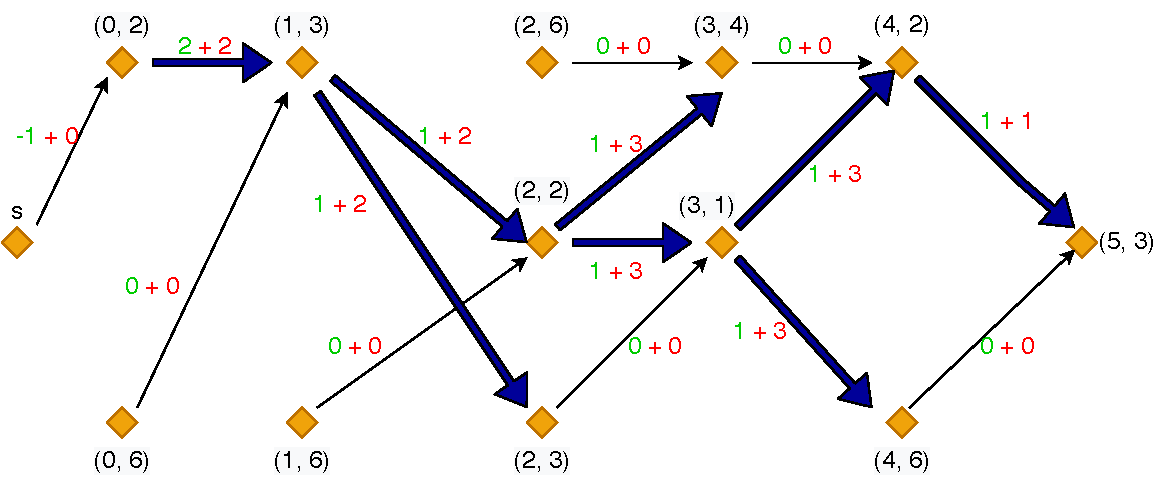
\includegraphics[height=7.5cm]{images_these/UsefulVDGraph.pdf}}
		\caption[Le sous-graphe Useful VD\_Subgraph]{Le sous-graphe \textbf{Useful VD\_Subgraph}.}
		\label{Useful_VD-Subgraph}
	\end{figure}
\end{Example}

La construction de \textbf{VD\_Graph} et le lemme \ref{Lemme_VD-Graph} nous permettent d'affirmer le théorème \ref{VD_polynomial}. %La démonstration de ce théorème se fait à la section suivante.
%\begin{theo}
%	\label{VD_polynomial}
%	\textbf{VD} peut être résolu en temps polynomial.
%\end{theo}


\textbf{Démonstration} : En raison du lemme \ref{Lemme_VD-Graph} et de la construction du sous-graphie \textit{Useful VD\_Subgraph} de la figure (\ref{Useful_VD-Subgraph}), nous voyons que résoudre \textbf{VD} signifie rechercher le plus court chemin de $s$ à $p$ dans le sous-graphie \textit{Useful VD\_Subgraph}. Mais, pour tout $j$, la cardinalité de $X(j)$ ne dépasse pas $M - j + 1$, et le nombre d'arcs qui relie $X(j)$ à $X(j+1)$ ne dépasse pas $Card(X(j) + Card(X(j+1))$. $\square$
}

%********************************************************************